%%%%%%%%%% ESPERANTO MANUAL %%%%%%%%%%%%%%%%%
\documentclass[a4paper,11pt]{book}
\usepackage[utf8x]{inputenc}
\usepackage{amsfonts,amsmath,amssymb,mathrsfs}
\usepackage{makeidx}
\usepackage[esperanto]{babel}
%% carleos: 
%% difinitaj en babel-french
\newcommand{\og}{{«}}
\newcommand{\fg}{{»}}
\newcommand{\degre}{{\ensuremath{^{\circ}}}}
%% pro stetiko
\usepackage{url}
%% fin-carleos
\usepackage[T1]{fontenc}
\usepackage{graphicx,ulem}
\usepackage{multicol,longtable,array}
\usepackage{colortbl,color}
\usepackage{pstricks,pstricks-add,pst-math,pst-xkey}
\usepackage{geometry}
\geometry{a4paper,tmargin=2cm,bmargin=2cm,rmargin=1.5cm,lmargin=1.5cm}
\newcommand{\logo}{\textsc{Logo}}
\newcommand{\xlogo}{\textsc{XLogo}}
\newcommand{\prim}[2]{%
%karleos forigas: \\
\noindent \begin{tabular}{>{\columncolor[gray]{0.9}}p{\textwidth}} 
\ifx \Css\UnDef\else
\Css{\#TBL-\TableNo {width:100\%;} }
\fi
\index{#1} \textbf{#1} \textit{#2}\\ 
\end{tabular} 
\\ 
}
\author{Loïc Le Coq}
\title{
\Huge \textbf{\xlogo: referenca gvidlibro}
}
\date{\today
\begin{center}
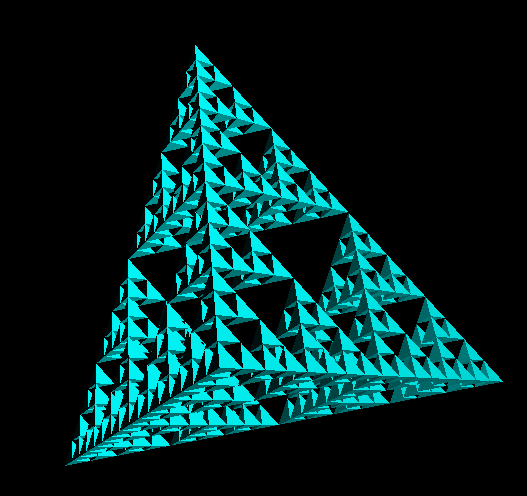
\includegraphics[scale=0.8]{bildoj/titolo.png}
\end{center}
\texttt{http://xlogo.tuxfamily.org}\\
}
\makeindex
\begin{document} 
\renewcommand{\labelitemi}{\textbullet}
\renewcommand{\labelitemiii}{$\rightarrow$}
\maketitle
\chapter*{Enkonduko}

Logo estas programlingvo disvolvata en la jaroj 60 de Seymour Papert.
Li apogis sin sur originala teorio pri la lernado, nomata konstruismo,
kies koncepton oni povas resumi per la esprimo
\og\textit{lerni-per-fari}\fg.

La lingvo \logo\ ebligas vaste disvolvi iujn matematikajn kaj logikajn
kapablojn; ^gi estas bonega lingvo por ekstudi la programadon kaj
lerni la bazojn kiel la buklojn, la provojn, la procedurojn...  La
uzulo povas movi objekton nomatan «testudo» sur la ekrano per komandoj
tiel simplaj kiel \texttt{anta^uen}, \texttt{malanta^uen},
\texttt{dekstren} kaj aliaj.  Post ^ciu movo, la testudo lasas ^spuron
malanta^u si kaj tiel oni povas krei desegnojn.  La fakto povi ordoni
en lingvo preska^u kutima faciligas multe la lernadon.  Anka^u pli
altnivela uzado eblas; oni povas manipuli objektojn tiajn kiel
listojn, vortojn a^u e^c dosierojn.

\logo\ estas lingvo interpretata, tio estas, la komandoj skribitaj de
la uzulo estas tuj rulotaj de la komputilo.  Oni rimarkas rekte de la
rulado de la programo, la erarojn faritajn; tio favoras la lernadon.

\xlogo\ estas do interpretilo por lingvo \logo.  La adreso de la ^cefa
loko de la programo estas:
\begin{center}
\texttt{http://xlogo.tuxfamily.org/}
\end{center}
Vi povos de^suti la programon kaj la dokumentaron.  Galerio de kelkaj
ekzemploj ebligas pli bone ekkoni la kapablojn de la programo.

\xlogo\ subtenas nun 10 lingvojn (angla, araba, astura, esperanto,
germana, hispana, franca, galega, greka kaj portugala) kaj estas
verkita en \textsc{Java}.  Tiu programlingvo havas la avanta^gon esti
plurplatforma, tio estas, ke la programo \xlogo\ ruli^gos sendepende
de la mastruma sistemo instalita.  ^Cu vi estas en GNU/Linukso, en
Vindozo a^u e^c en Makinto^so, ne estas problemo; la malgranda testudo
sin oferas al vi!\\

\noindent \textbf{\xlogo\ estas sub permesilo GPL:} \\ \\
^Gi estas do libera programo; tio garantias al la uzulo:
\begin{enumerate}
 \item la liberecon ruli la programon, por ia ajn celo;
 \item la liberecon studi la funkciadon de programo kaj adapti ^gin al
   siaj bezonoj; tio postulas alireblon al la fontokodojn;
 \item la liberecon disdoni kopiojn;
 \item la liberecon plibonigi la programon kaj publikigi la modifojn
   por ke la tuta komunumo profitu.
\end{enumerate}
\noindent \textbf{Strukturo de la gvidlibro:}\\ \\
Tiu gvidlibro ebligos vin ekkoni \xlogo n.
\begin{itemize}
\item La unua parto estas dedi^cita al priskribo de la interfaco kaj
  de la diversaj menuoj.
\item Poste, kelkaj ^capitroj al vi prezentas la unuajn bazajn
  instrukciojn de \xlogo.  La malfacileco de la en^cenado de la nocioj
  estas gradita.  Ekzercoj aplikaj estas proponataj je la fino de
  ^capitro; iliaj korektigoj estas en krom^capitro.
\item Finfine, kelkajn specialajn temojn oni traktas por la altnivelaj
  uzuloj.
\item En krom^capitro, vi trovos la priskribon de ^ciuj primitivoj,
  kaj la diversajn elekta^jojn por ekruli \xlogo n.
\end{itemize}
\vspace{0.5cm}
^Ci tiu gvidlibro haveblas en diversaj formatoj:
\begin{itemize}
 \item \textsc{PDF}: http://downloads.tuxfamily.org/xlogo/downloads-eo/manual-eo.pdf
 \item \textsc{HTML zipita}: http://downloads.tuxfamily.org/xlogo/downloads-eo/manual-html-eo.zip
 \item \LaTeXe: Fontokodo de la gvidlibro: http://downloads.tuxfamily.org/xlogo/downloads-eo/manual-src-eo.zip
 \item \textsc{JavaHelp}: Per la menuo Helpo-Gvido dumrule de \xlogo
\end{itemize}

\tableofcontents
\chapter{Instalado de \xlogo}
\noindent 
\begin{itemize}
 \item Unue, vi bezonas instali rulmedion JAVA en via komputilo.  Iru al tiu pa^go:
\begin{center}
 \texttt{http://java.sun.com/javase/downloads/index.jsp}
\end{center}
De^sutu la JRE (Java Runtime Environment) korespondantan al via
mastruma sistemo (Vindozo, GNU/Linukso...); poste instalu ^gin.
\item Due, necesas de^suti la dosieron \texttt{xlogo.jar} estanta ^ce
  la adreso:
\begin{center}
 \texttt{http://downloads.tuxfamily.org/xlogo/common/xlogo.jar}
\end{center}
Se ne, pli simple, iru al la loko de \xlogo, ^ce la adreso
\texttt{http://xlogo.tuxfamily.org}; poste elektu la lingvon kaj la
menuon de^suti.
\end{itemize}
\section{Agordado de \xlogo}
\subsection{Medio GNU/Linukso}
En Ubuntu 8.04:
\begin{enumerate}
 \item Por instali JAVA:
\begin{itemize}
\item Sistemo -> Administri -> Administrilo de pakoj Synaptic
\item Instali la pakon \texttt{sun-java6-jre}
\end{itemize}
\item Por malfermi la dosieron \texttt{xlogo.jar} per duobla klako:
\begin{itemize}
\item Dekstreklaku sur \texttt{xlogo.jar}, Atributoj
\item Tabo \og Malfermi per\fg: Elektu Sun Java Runtime 
\end{itemize}
 \item Asociigu la dosiertipon \texttt{lgo} al \xlogo:
\begin{itemize}
 \item Dekstreklaku sur \texttt{xlogo.jar}, Atributoj
 \item Tabo \og Malferm per\fg:
 \item Butono \og Aldoni\fg
 \item En \og Uzi komandon personigitan:\fg, tajpu:
\begin{center}
\texttt{java -jar vojo\_al\_xlogo.jar} 
\end{center}
\end{itemize}
\end{enumerate}
\textbf{Rimarku:} \xlogo\ estas enhavita en la distribuo OpenSuse.
\subsection{Medio Windows}
Komence, se vi duobleklakas sur la ikono de \xlogo, la programo devas
starti.  Se ^gi okazas, iru al la sekva paragrafo.  Se ne, la ka^uzo
estas ke alia programo okupi^gas pri la dosierojn de tipo
\og\texttt{jar}\fg\ (ofte, malkunpremaj programoj, kiel WinZip kaj
aliaj).

Jen kiel asociigi la programon \og\texttt{java}\fg\ al la dosieroj de
tipo \og \texttt{jar}\fg.  (Kelkaj vojoj povas esti malsamaj, la^u ke
vi posedas Vindozo 98, 2000, XP...)
\begin{enumerate}
\item Starto –> Parametroj —> Elekto de dosieroj...
\item Klaku poste sur la tabo \og Dosiertipoj\fg\ (la
  3\textsuperscript{a}).
\item Ser^cu en la listo la elekta^jojn rilatajn al dosieroj JAR
  (Dosieroj JAR, Ruldosieroj JAR, Ar^hivo JAR...)
\item Elektu tiun dosiertipon kaj klaku sur \og Modifi...\fg 
\item Nova fenestro aperas, tiam elektu \og Modifi... \fg 
\item Elekt tiam \og Traser^ci...\fg
\item Necesas indiki la vojon al \texttt{javaw.exe}, ekzemple
\begin{center}
 \texttt{c:\textbackslash Program Files\textbackslash java\textbackslash j2re1.4.1\textbackslash bin\textbackslash javaw.exe}
\end{center}
\item Tion farinte, aperas en la kampo Aplika^jo uzata por efektivigi
  la agon:
\begin{center}
 \texttt{c:\textbackslash Program Files\textbackslash java\textbackslash j2re1.4.1\textbackslash bin\textbackslash javaw.exe}
\end{center}
Necesas tiam aldoni ^ce la fino:
\begin{center}
\texttt{"c:\textbackslash Program Files\textbackslash java\textbackslash j2re1.4.1\textbackslash bin\textbackslash javaw.exe" -jar "\%1" \%*}
\end{center} 
(Rimarku ke necesas spaceto je ^ciu flanko de -jar)
\item Poste, nur fermu ^ciun fenestron kaj poste duobleklaku sur la
  ikono de \xlogo.
\end{enumerate}
Se tio ne ^ciam funkcias, estas dua eblo: Vi malfermu konsolon MSDOS
(Starto --> Programoj -–> Komandoj MSDOS a^u Starto --> Programoj -->
Iloj --> Invito MSDOS); poste tajpu la ordonon jenan:
\begin{center}
 \texttt{java -jar la\_vojo\_kie\_trovi^gas\_la\_dosiero}
\end{center}
Por ekzemplo: \texttt{java -jar c:\textbackslash xlogo\textbackslash xlogo.jar}\\ \\
Se tio enuas vin, sisteme devi tajpi tiun ordonon, tajpu tion en
teksta dosiero kaj konservu ^gin ekzemple sub la nomo
\texttt{xlogo.bat}.  Nur restas duobleklaki sur \texttt{xlogo.bat} por
startigi \xlogo n.

\subsubsection*{Asociigi la dosierojn de tipo \texttt{lgo} kun \xlogo}
Mi ne atingis agordi tion en Vista.  (Sed mi ne tre ser^cis...
Rimarku, amatoroj!  Dankon pro komuniki al mi la solvon.)

Principe, la dosieroj de tipo \texttt{.lgo} ne estas rekonataj de via
komputilo; kiam vi duobleklakas ilin, dialogskatolo aperas por demandi
al vi kiun aplika^jon oni uzu por malfermi la dosieron.
\begin{itemize}
\item Indiku \og Alia\fg; poste indiku la vojon al la programo
  \texttt{javaw.exe}
\begin{center}
^Generale, \texttt{c:\textbackslash Program Files\textbackslash java\textbackslash j2re1.4.1\textbackslash bin\textbackslash javaw.exe}
\end{center}
\item Doni nomon por nomi la dosierojn je tipo \texttt{lgo}.\\
Por ekzemplo: Dosieroj Logo
\item Starto -> Parametroj -> Agorda^joj de la dosieroj
\item Tabo \og Dosiertipoj \fg
\item Ser^cu en la listo la dosierojn \texttt{lgo}
\item Elektu tiun dosiertipojn; poste klaku sur \og Modifi\fg
\item Nova fenestro aperas; refoje \og Modifi\fg
\item En la kampo \og Aplika^jo uzata por efektivigi la agon\fg,
\begin{center}
\texttt{"c:\textbackslash Program Files\textbackslash java\textbackslash j2re1.4.1\textbackslash bin\textbackslash javaw.exe" -jar xlogo.jar "\%1" \%*}
\end{center} 
\item Fermu la fenestrojn.
\end{itemize}
\section{^Gisdatigoj}
\begin{center}

\includegraphics{bildoj/rss.png} \hspace{1cm} \texttt{http://xlogo.tuxfamily.org/rss.xml}
\end{center}
Por ^gisdatigi \xlogo, sufi^cas anstata^uigi la dosieron
\texttt{xlogo.jar} per ^gia nova versio.  Se vi deziras esti avertata
de la apero de ^ciu nova versio, a^u de ^ciu plibonigo, eblas aboni al
la RSS-fadeno de \xlogo.  La adreso de la RSS-fadeno estas:
\begin{center}
 \texttt{http://xlogo.tuxfamily.org/rss.xml}
\end{center}
Ekzistas pluraj softvoj ebligantaj sekvi la fadenojn RSS; se vi ne
konas tiun te^hnikon, la plej simpla estas uzi Mozilla Thunderbird:
\begin{itemize}
 \item Menu' Redakti - Parametroj de la kontoj
 \item Buton' \og Aldoni konton\fg
 \item \og Nova^joj RSS kaj blogoj\fg
 \item Nomo de la konto: \og Fadenoj RSS\fg\ por ekzemplo
 \item Butonoj \og Sekva\fg\ kaj \og Fini\fg
 \item En la fenestro \og Parametroj de la kontoj\fg, elektu tiam \og
   Fadenoj RSS\fg\ en la menu' maldekstra; poste klaku sur la butono
   \og Administri la abonoj\fg.
 \item Buton' \og Aldoni\fg
	\begin{itemize}
 	\item URL de la fadeno: \texttt{http://xlogo.tuxfamily.org/rss.xml}
	\item Aktivigu la skatolon \og Afi^si la resumon de l'
          artikolo anstata^u de^suti la retpa^gon\fg
	\end{itemize}
\end{itemize}
\vspace*{0.2cm} Jen, per la butono \og Sendi-Ricevi\fg, vi ricevos la
nova^jojn de \xlogo\ sammaniere kiel vi ricevas viajn retpo^sta^join.
\section{Malinstalado}\label{fichier_perso}
Por malinstali \xlogo, sufi^cas forigi la dosieron \texttt{xlogo.jar}
kaj la startan dosieron \texttt{.xlogo} (^gi estas lokita en via uzula
dosierujo, tio estas, \texttt{/home/via\_konto} por la gnulinuksistoj
a^u \texttt{c:\textbackslash windows\textbackslash.xlogo} por la
vindozistoj.

\chapter{Prezentado de l' interfaco:}
\section{Je la unua ekrulado}
Je la unua fojo kiam vi ekrulas Xlogon (a^u se vi forigis la dosieron
\texttt{.xlogo} --- rigardu sekcion \ref{fichier_perso}),
dialogfenestro aperas por ebligi vin elekti la lingvon uzotan.
\begin{center}
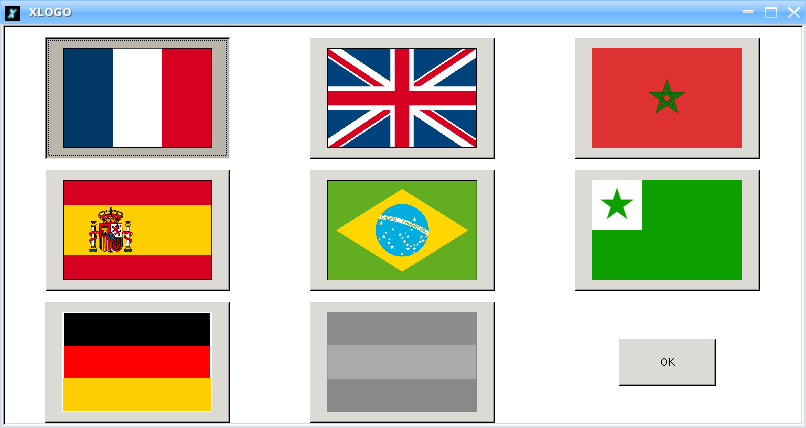
\includegraphics[scale=0.2]{bildoj/CaptureLangue.png} 
\end{center}
Tiu elekto ne estas definitiva, kompreneble; ^gin oni povas korekti
tuj per helpo de la dialogfenestro Preferoj (rigardu sekcion
\ref{onglet_general}).
\section{^Cefa fenestro}
\begin{center}
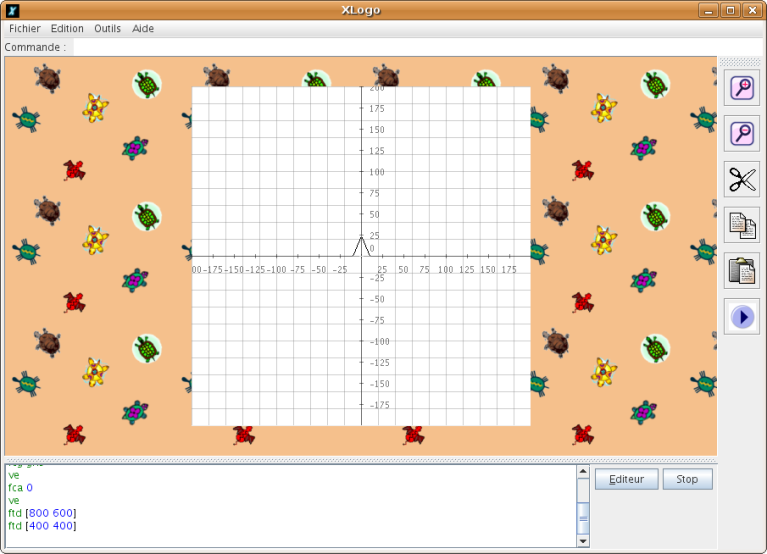
\includegraphics[scale=0.45]{bildoj/Capture.png} 
\end{center}
\begin{itemize}
\item Supre, la tradiciaj menuoj \begin{large} \textbf{Dosiero},
    \textbf{Redakti}, \textbf{Iloj} kaj \textbf{Helpo} \end{large}
\item Apude sube, \textbf{\begin{large}la komandlinio\end{large}}
  ebliganta skribi la logo-instrukciojn.
\item Meze, \begin{large}\textbf{la areo por desegni}\end{large}.
\item Dekstre de la desegnareo,
  \textbf{\begin{large}ilbreto\end{large}} vin ebligas realigi
  diversajn agojn:
\begin{itemize}
\item Zomi anta^uen/posten.
\item Diversaj redaktaj kapabloj (fortondi/kopii/alglui, tio estas,
  forigi/enpo^sigi/elpo^sigi).
\item La butono \og Legi\fg\ ebligas ruli la ^cefan komandon difinitan
  en la redaktilo.
\end{itemize}
\item Malsupre, \begin{large}\textbf{la areo \og historia
      \fg}\end{large} \ kiu memoras ^ciun lastajn komandojn tajpitajn
  kaj la respondojn rilatajn.  Por reskribi rapide instrukcion jam
  tajpitan, estas du solvoj: ^cu klaki sur la malnova instrukcio en la
  historia, ^cu klaki plurfoje sur la sago supra ^gis la instrukcio
  dezirata aperos.  La du sagoj supra kaj malsupra efektive ebligas
  movi^gi tra la tuta historio de la anta^ue tajpitaj komandoj (tre
  utile).
\item Dekstre de l' historio, du butonoj: \begin{large}\textbf{HALTI}
    kaj \textbf{REDAKTILO} \end{large}.
\begin{itemize}
\item La butono HALTI haltas ^ciun ruladon kurantan.
\item La butono REDAKTILO ebligas malfermi la proceduran redaktilon.
\end{itemize}
\end{itemize}
\section{La proceduran redaktilon}
\begin{center}
 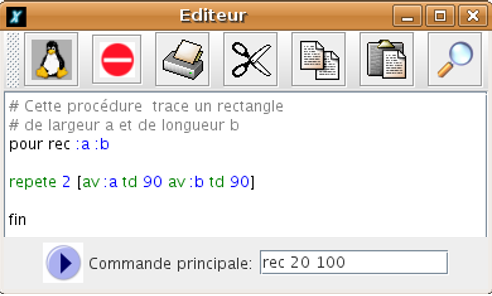
\includegraphics[scale=0.4]{bildoj/CaptureEditeur.png}
\end{center}
Por malfermi la redaktilon, tri ebloj:
\begin{itemize}
\item Tajpi \texttt{ed} en la komandlinio.  La redaktilo malfermi^gos
  tiam kun ^ciuj proceduroj jam difinitaj.  Se vi nur deziras redakti
  kelkajn procedurojn, tajpu tiam:\\
  \texttt{ed [proceduro\_1 proceduro\_2 ...]}
\item Klaku sur la butono Redaktilo de la ^cefa fenestro.
\item Uzu la klavkombinon Alt+E
\end{itemize} 
\vspace{0.5cm}
Jen la diversaj butonoj kiujn vi trovos en la redaktilo:\\

\begin{longtable}{cm{12cm}}
  \includegraphics*[scale=1]{bildoj/tortue.png} &
  Konservi la modifojn de la enhavo de la redaktilo, poste ^ci tiun
  fermi.  Ja sur tiu butono oni klaku ^ciufoje ke oni volas konservi
  la tajpitajn procedurojn.  Se vi preferas, vi povas uzi la
  klavkombinon ALT+Q. \\
  \includegraphics*[scale=1]{bildoj/quit.png} &
  Eliru la redaktilon konservante neniun modifon faritan en tiu.  Oni
  anka^u povas uzi la klavkombinon ALT+C. \\
  \includegraphics*[scale=1]{bildoj/fileprint.png} & 
  Presi la enhavon de la redaktilo.\\
  \includegraphics*[scale=1]{bildoj/editcopy.png} & 
  Kopii la elektitan tekston en la po^son.\\
  \includegraphics*[scale=1]{bildoj/editcut.png} & 
  Meti la elektitan tekston en la po^son.\\
  \includegraphics*[scale=1]{bildoj/editpaste.png} & 
  Kopii la elektitan tekston de la po^so.\\
  \includegraphics*[scale=1]{bildoj/chercher.png} &
  Malfermu dialogfenestron ebligantan ser^ci a^u anstata^uigi tekston
  en la redaktilo. \\
\end{longtable} 
\begin{center}
 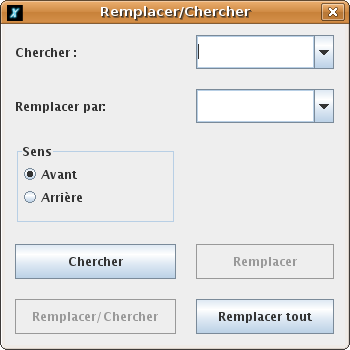
\includegraphics[scale=0.4]{bildoj/CaptureChercher.png}
\end{center}
\vspace{0.5cm}

\includegraphics{bildoj/play.png}
Malsuprege de la redaktilo, teksta kampo ebligas difini ^cefan
komandon.  ^Ci tiu reprezentas la ^generalan komandon ebligantan ruli
programon.  ^Gi estas atingebla per la butono \og legado\fg\ de la
ilbreto en la ^cefa fenestro.  Kiam oni konservas la enhavon de la
redaktilo en dosieron kun formato \texttt{.lgo}, anka^u tiu komando 
estas konservata \\ \\
\textbf{\begin{Large}GRAVE\end{Large}}: \\
\begin{itemize}
\item Neniel utilas klaki la krucon supre dekstre por fermi la
  fenestron!  Nur la du unuaj butonoj permesas eliri el la redaktilo.
\item Por forigi unu a^u plurajn procedurojn nedezirataj, uzu la
  primitivon \texttt{efp, effaceprocedure} a^u klaku en la
  menubreto \textbf{Iloj - Gestionnaire de procédures}.
\end{itemize} 
\section{Quitter}
Por eliri el XLogo, en la menubreto \textbf{Dosiero - For}, a^u klaku
la ferman krucon de la fenestro.  Dialogfenestro por konfirmi aperas
je tiu momento.
\begin{center}
 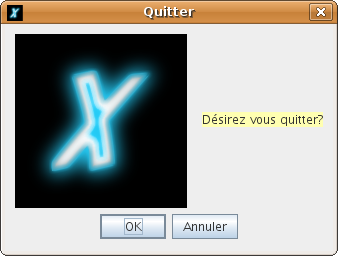
\includegraphics[scale=0.4]{bildoj/CaptureQuitter.png}
\end{center}
\chapter{Elektebloj de la menuoj:}
\section{Menu' \og Dosiero\fg}
\begin{itemize}
\item \textbf{Dosiero$\to$Nova}: detruas ^ciujn procedurojn kaj
  variabloj difinitajn por krei tiele novan laborspacon.
\item \textbf{Dosiero$\to$Malfermi}: malfermas logo-dosieron anta^ue
  konservitan.
\begin{center}
 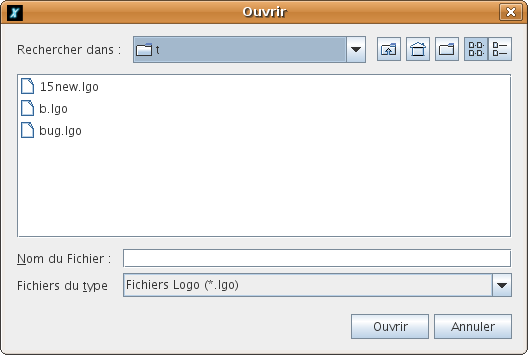
\includegraphics[scale=0.4]{bildoj/CaptureOuvrir.png}
\end{center}
\vspace{0.25cm}
\item \textbf{Dosiero$\to$Konservi kiel...}: konservas la kurantajn
  procedurojn sub elektitan nomon.
\begin{center}
 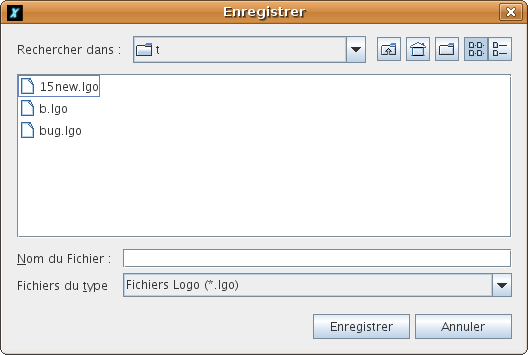
\includegraphics[scale=0.4]{bildoj/CaptureEnregistrer.png}
\end{center}
\vspace{0.25cm}
\item \textbf{Dosiero$\to$Konservi}: konservas la proceduroj en la
  dosieron nun uzatan.
\item \textbf{Dosiero$\to$Kapti la bildon$\to$Konservi la bildon
    kiel...}: ebligas konservi la bildon kun formato jpg a^u png.  Se
  vi deziras elekti nur parton de l' bildo, eblas difini elektan
  ortangulon per gliti la muson sur la desegna areo.
\item \textbf{Dosiero$\to$Kapti la bildon$\to$Presi la bildon}:
  ebligas presi la bildon.  Kiel la anta^ua, vi povas elekti ^gustan
  areon presotan.
\item \textbf{Dosiero$\to$Kapti la bildon$\to$Kopii la bildon en la
    po^son}: Ebligas sendi la bildon en la po^san sistemon.  Kiel por
  presi kaj konservi, vi povas anka^u elekti nur areon de la bildo.
  ^Gi funkcias bone en Vindozo, ne en Linukso, ne provita en
  Makinto^so.
\item \textbf{Dosiero$\to$Tekstareo$\to$Konservi je formato RTF}:
  Ebligas konservi la historian areon je formato RTF (konservas la
  kolorojn kaj formatadon de la signoj).
\item \textbf{Dosiero$\to$Eliri}: Eliri el la programo XLOGO.
\end{itemize}

\section{Menu' \og Redakti\fg}
\begin{itemize}
\item \textbf{Redakti$\to$Kopii}: Kopias la elektitan tekston en la
  po^son.
\item \textbf{Redakti$\to$Fortran^ci}: Movas la elektitan tekston en
  la po^son.
\item \textbf{Redakti$\to$Alglui}: Elpo^sigas la tekston en la
  komandlinion.
\item \textbf{Redakti$\to$Elekti ^cion}: Elektas la tutan tekston de
  la komandareo.
\end{itemize}

\section{Menu' \og Iloj\fg}
\begin{itemize}
\item \textbf{Iloj$\to$Elekti krajonan koloron}: Ebligas elekti la
  koloron per kiu skribas la testudo, helpe de koloraro.
\begin{center}
 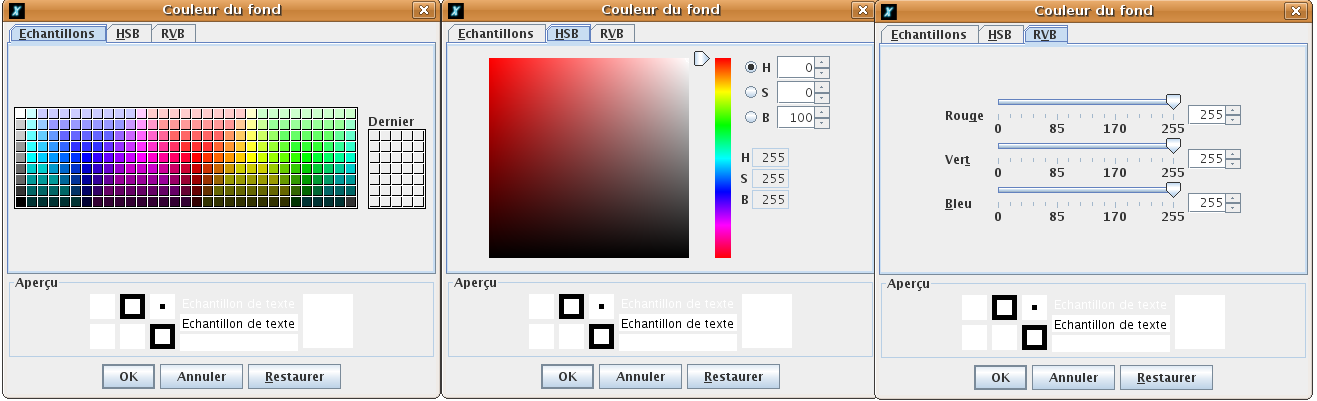
\includegraphics[scale=0.3]{bildoj/CaptureCouleur.png}
\end{center}
\vspace{0.25cm}
Havebla anka^u per la primitivo \texttt{fcc} (rigardu kroma^jon \ref{fcc}).
\item \textbf{Iloj$\to$Elekti fonkoloron}: Same pri la ekranfono.
  Havebla per la primitivo \texttt{fcfg} (rigardu kroma^jon \ref{fcfg}).
\item \textbf{Iloj$\to$Difini startodosierojn}: ebligas difini vojojn
  al dosieroj kun formato *.lgo nomataj \og startecaj\fg.  ^Ciuj
  proceduroj en tiuj dosieroj esti^gos \og kvaza^u-primitivoj\fg \ de
  la lingvo XLogo.  Ili ne estas redakteblaj nek modifeblaj de l'
  uzulo.  Vi povas anka^u difini personigitajn primitivojn.  Vi povas
  anka^u doni al ^gi komandon (en logo) rulatan dum starto de XLogo.
  Vi povas anka^u ruli programon koncipitan de vi, ekde la malfermo de
  XLogo.
  \begin{center}
    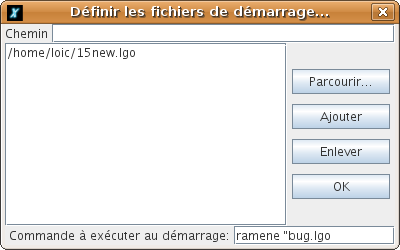
\includegraphics[scale=0.4]{bildoj/CaptureDemarrage.png}
  \end{center}
  \vspace{0.25cm}
\item \textbf{Iloj$\to$Traduki procedurojn}: Malfermas dialogfenestron
  ebligantan traduki komandojn XLogo en la lingvon deziratan.  (Tre
  utila speciale kiam oni prenas en interreto Logo-fontokodon en la
  angla, por ilin esperantigi.)
\begin{center}
 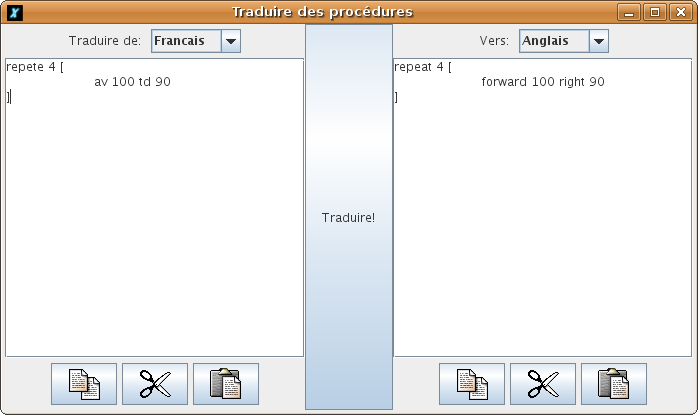
\includegraphics[scale=0.4]{bildoj/CaptureTraduire.png}
\end{center}
\vspace{0.25cm}
\item \textbf{Iloj$\to$Procedura administrilo}: Malfermas
  dialogfenestron kiu ebligas forigi procedurojn.  ^Gi permesas anka^u
  ^san^gi la aperordon de la proceduroj en la redaktilo.
\begin{center}
 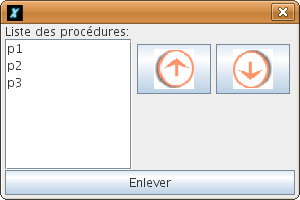
\includegraphics[scale=0.4]{bildoj/CaptureProcedure.png}
\end{center}
\vspace{0.25cm}
\item \textbf{Iloj$\to$Preferoj}: Malfermu dialogfenestron en kiu vi
  povas agordi plurajn aferojn:
  \begin{itemize} 
  \item \textbf{^Generala langeto:} \label{onglet_general}
    \begin{itemize}
    \item \textbf{Lingvo}: ^Gi ebligas elekti inter la franca, la
      angla, la hispana, la portugala, l' araba, la germana kaj
      esperanto.  Atentu, ^car la primitivoj ^san^gi^gas de lingvo al
      alia.
    \item \textbf{Aspekto:} Ebligas difini la \og look\fg on\ de la
      fenestro XLogo.  ^Cu stilo nativa, ^cu stilo Java (metala), ^cu
      stilo Motif.
    \item \textbf{Elekti la skribrapidon:} Se vi deziras vidi ^ciun
      transloki^gon de la testudo, vi povas malrapidigi ^gin helpe de
      la glitbutono celita por tio.
      \begin{center}
        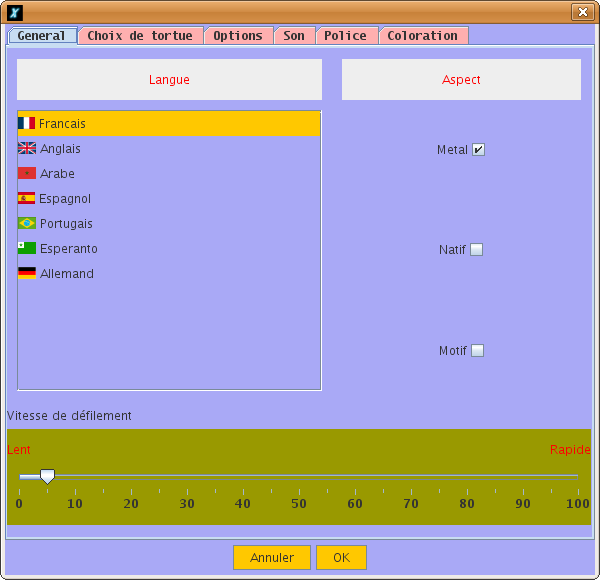
\includegraphics[scale=0.3]{bildoj/CapturePref1.png}\\
        \vspace*{1cm}
        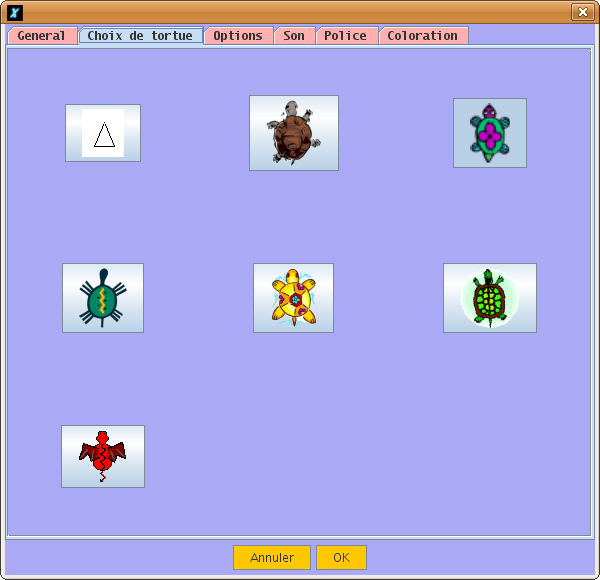
\includegraphics[scale=0.3]{bildoj/CapturePref2.png}
      \end{center}
      \vspace{0.25cm}
    \end{itemize}
  \item \textbf{Langeto Elekti testudon}: Vi povas elekti vian preferatan
    testudon.
    \begin{center}
      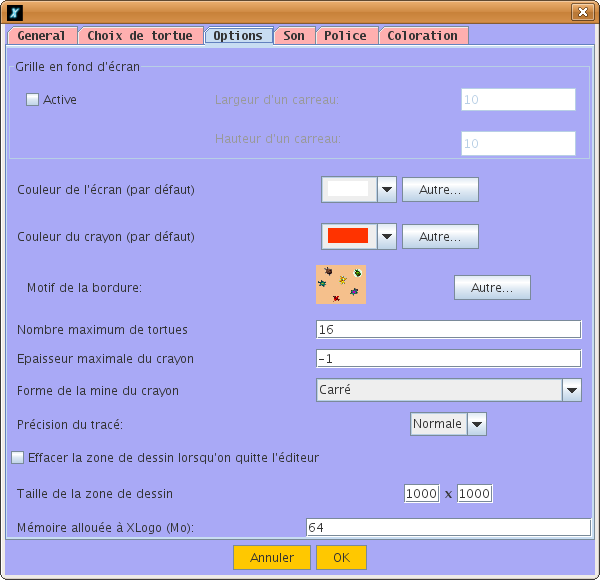
\includegraphics[scale=0.4]{bildoj/CapturePref3.png}
    \end{center}
  \item \textbf{Langeto Elektoj}: Oni povas agordi plurajn aferojn. 
    \begin{itemize}
    \item \textbf{Dratreto:} Vi povas elekti ^cu desegni dratreton sur
      l' ekranfono.  Vi povas elekti la lar^gon kaj la alton de
      kvadrato de la dratreto, kaj anka^u ^gian koloron.
    \item \textbf{Aksoj:} Vi povas elekti ^cu desegni la vertikalan
      akson kaja^u la horizontalan akson sur l' ekranfono.  Vi povas
      difini la distancon inter du gradumoj kaj anka^u la koloron de
      ^ciu akso.
    \item \textbf{Koloro de ekranfono}: Eblo difini aprioran koloron
      de ekranfono.
    \item \textbf{Koloro de krajono}: Eblo difini aprioran koloron
      krajonan.
    \item \textbf{Bordera motivo}: Eblo difini preciza motivon por la
      mar^geno enkadriganta la desegnejon (^cu per bildo, ^cu per nura
      koloro)
      \begin{center}
        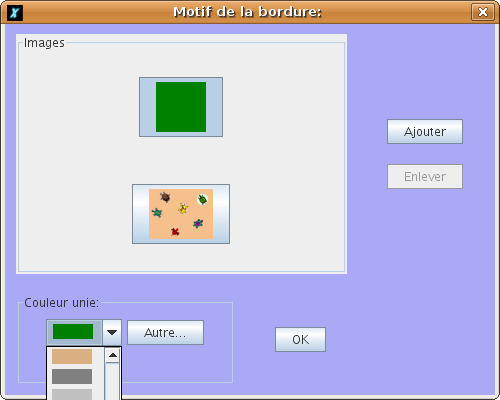
\includegraphics[scale=0.4]{bildoj/CaptureBordure.png}
      \end{center}
    \item \textbf{Diko de krajono}: Oni povas indiki liman amplekson
      por la dikeco de krajono.  Si oni ne volas uzi tiun limigon,
      metu la nombron $-1$ en la areon tekstan rilatan.
    \item \textbf{Formo de krajono}: Tuj, oni povas elekti la formon
      de la testuda krajono.  Por ^gin rimarki, elektu krajondikon pli
      grandan ol $1$.
    \item \textbf{Maksimuma nombro de testudoj}: Oni povas ^san^gi la
      maksimuman nombron de testudoj en plurtestuda moduso (apriore
      16).
    \item \textbf{Desegna precizeco}: Vi povas elekti la desegnan
      kvaliton.  Je alta kvalito, vi ne havos la efikon de
      linipikselado.  Male, atentu ke, ju pli da kvalito, des malpli da
      rulrapideco.
    \item \textbf{Purigado je eliro el redaktilo}: Oni povas elekti
      ^cu a^utomate purigi la desegnejon kiam oni eliras el la
      redaktilo.
    \item \textbf{Amplekso de la desegnejo}: Vi povas elekti propran
      amplekson por la desegnejo.  Apriore XLogo ruli^gas kun areo de
      1000 pikseloj mul 1000 pikseloj. \textcolor{red} {Atentu:} Kiam
      vi pligrandigas la bildon, eble necesas pligrandigi la kvanton
      de memoro atribuita al XLogo.  Erarmesa^go vin avertos pri tio.
    \item \textbf{Memoro atribuita al XLogo}: Vi povas tial anka^u
      ^san^gi la valoron rilatan al la memora spaco atribuita al
      XLogo.  Apriore, tiu valoro estas 64 MiB.  Eble vi devos
      pligrandigi ^gin se vi deziros labori sur desegnejo pli granda.
      Kiam oni modifas tiun parametron, la ^san^go nur efikas post la
      restarto de XLogo. \textcolor{red} {Atentu, ne pligrandigu multe
        sen ka^uzo tiun valoron; ^gi povas multe malrapidigi vian
        sistemon.}
    \item \textbf{Nombro de pordo TCP:} Ebligas elekti iun valoron por
      la pordo uzata por la retkomunikadoj.  Rigardu
      p.~\pageref{reseau}.
    \end{itemize}
    \begin{center}
      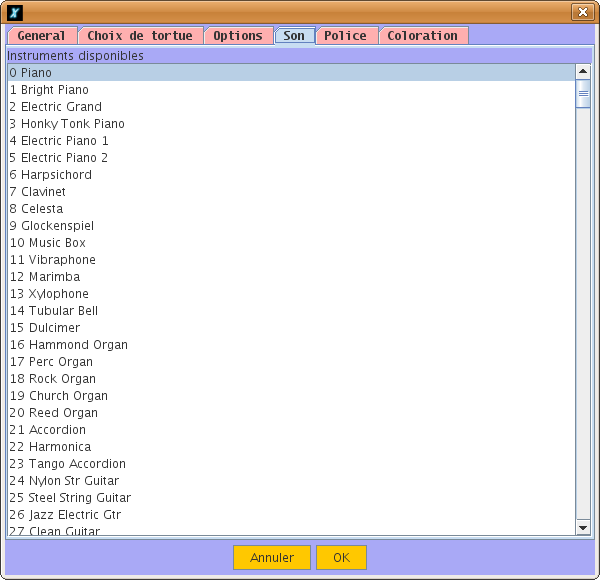
\includegraphics[scale=0.4]{bildoj/CapturePref4.png}
    \end{center}
    \vspace{0.25cm}
  \item \textbf{Langeto Sono}: vi trovos la liston de instrumentoj
    kiujn povas ^sajnigi via sonkarto per l' interfaco MIDI.  Vi povas
    elekti instrumenton klakante ^gian nomon.  (Vi povas elekti
    instrumenton anka^u per la primitivo \texttt{instrumenton\_provizu
      numero}.)  Se la listo de instrumentoj ne aperas, rigardu la
    Oftajn Demandojn fine de l' gvidlibro pri tiu afero.
    \begin{center}
      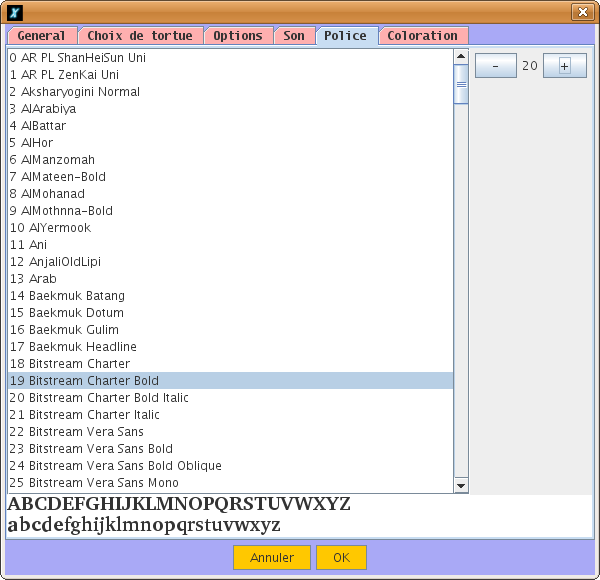
\includegraphics[scale=0.4]{bildoj/CapturePref5.png}
    \end{center}
    \vspace{0.25cm}
  \item \textbf{Langeto Tiparo}: En la kvina langeto, vi povas elekti
    la tiparon de la grafika interfaco kaj ^gian amplekson.  Atentu ke
    tio ne influas la tiparon uzatan de la primitivoj \texttt{skribu}
    et \texttt{etikedu}.
    \begin{center}
      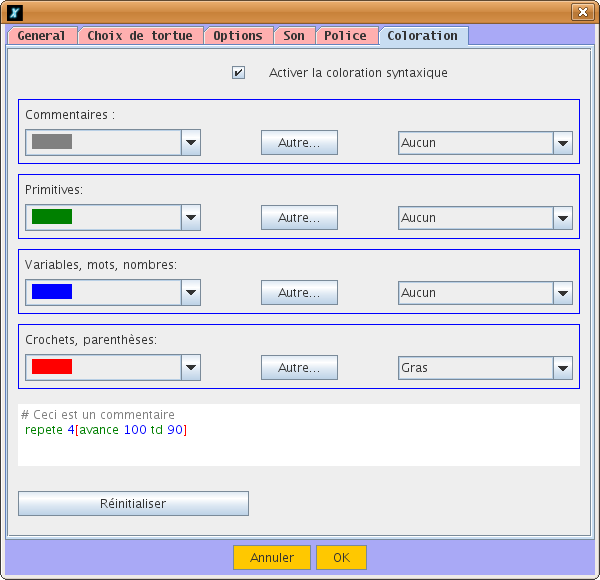
\includegraphics[scale=0.4]{bildoj/CapturePref6.png}
    \end{center}
    \vspace{0.25cm}
  \item \textbf{Langeto Sintaksa kolorigo}: Eblo (mal)aktivigi la
    sintaksan kolorigon kaj difini proprajn kolorojn.
\end{itemize}
\end{itemize}
\section{Menu' \og Helpo\fg}
\begin{itemize}
\item \textbf{Menu' Helpo$\to$Reta lernolibro}: Aliras la referencan
  lernolibron de \xlogo, nur se ekzistas interreta konekto.
  \vspace{0.25cm}
\item \textbf{Menu' Helpo$\to$Permesilo}: Aliras la permesilon GPL sub
  kiu oni distribuas la programon.
  \begin{center}
    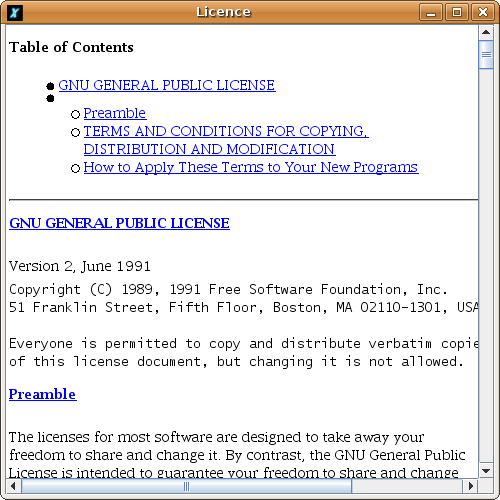
\includegraphics[scale=0.4]{bildoj/CaptureLicence.png}
  \end{center}
  \vspace{0.25cm}
\item \textbf{Menu' Helpo$\to$Esperanta traduko}: Aliras
  esperantigitan permesilon GPL.  Tiu traduka^jo havas nenian valoron
  oficialan, nur la angla originalo.

\item \textbf{Menu' Helpo$\to$Traduki XLogo-n}: Malfermas
  dialogfenestron ebligantan konsulti / modifi / kompletigi la aron de
  traduka^joj de XLogo (mesa^goj kaj primitivoj).
  \begin{center}
    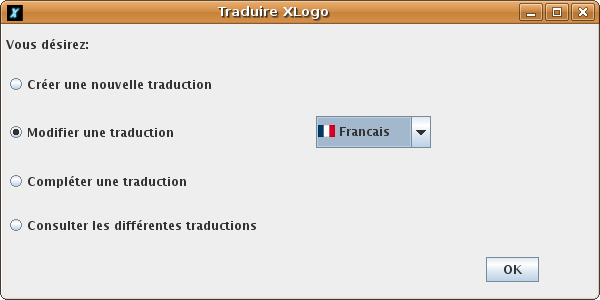
\includegraphics[scale=0.4]{bildoj/CaptureXLogoTrad1.png}
    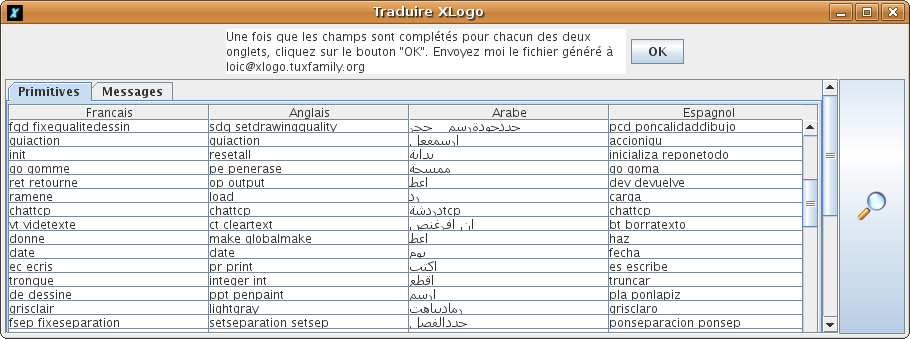
\includegraphics[scale=0.4]{bildoj/CaptureXLogoTrad2.png}
  \end{center}
  \vspace{0.25cm} Eblas anka^u krei traduka^jojn por nova
  lingvo.  Je ^ciu okazo oni sendu la dosieron generitan al
  \url{loic@xlogo.tuxfamily.org}.
\item \textbf{Menu' Helpo$\to$Rilate...}: Klasika ... kaj
  \url{http://xlogo.tuxfamily.org} por viaj ^gisdatigoj!!
  \texttt{o:)}
  \begin{center}
    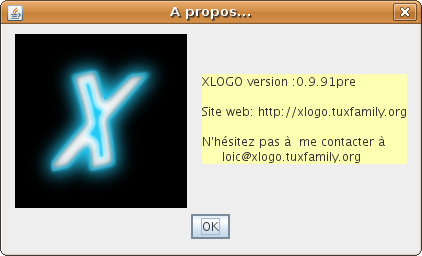
\includegraphics[scale=0.6]{bildoj/CaptureApropos.png}
  \end{center}
  \vspace{0.25cm}
\end{itemize}



\chapter{Konvencioj adoptitaj en XLOGO}
Jen prezentado de iuj aferoj pri la programlingvo LOGO mem kaj de
aliaj pri XLOGO specife.

\section{Komandoj kaj interpretado}
Programlingvo LOGO konsistas el internaj komandoj: tiajn komandojn oni
nomas \textbf{primitivoj}.  ^Ciu primitivo atendas iun nombron de
parametroj nomataj \textbf{argumentoj}.  Por ekzemplo, la primitivo
\texttt{ev} kiu ebligas vi^si l' ekranon prenas nul argumenton, dum la
primitivo \texttt{sum} atendas du argumentojn: \texttt{ sum 2 3}
skribos 5 redone.

Estas tri specoj de argumentoj en LOGO:
\begin{itemize}
\item \textbf{La nombroj:} Iuj primitivoj atendas nombrojn kiel
  argumenton.  Ekzemple \texttt{anta^uen 100}
\item \textbf{La vortoj:} ^Ciuj vortoj komenci^gas per ".  Ekzemplo de
  primitivo kapabla labori pri vortoj estas la primitivo
  \texttt{skribu}.
\begin{center}
\texttt{skribu "saluton} 
\end{center}
Tiu komando ka^uzas l' aperon de la vorto \texttt{saluton} en la
teksta areo.

Rimarku ke se vi forgesas la ", l' interpretilo respondos per
erarmesa^go.  Efektive, \texttt{skribu} atendas argumenton, sed por l'
interpretilo \texttt{saluton} signifas nenion, ^car ^gi estas nek
nombro nek vorto nek listo nek jam difinita proceduro.
\item\textbf{La listoj:} Ilin oni difinas inter rektaj krampoj.
\end{itemize}
\vspace{0.5cm} \textbf{Rimarku:} La nombroj estas traktataj jen kiel
nombraj valoroj, jen kiel vortoj.  Ekzemple: \texttt{skribu unuan 12}
redonas 1.  Iuj primitivoj akceptas ^generalan formon, tio estas, ili
povas ricevi nedifinitan nombron de argumentoj.  Jen la listo de tiuj
primitivoj:
\begin{center}
  \begin{tabular}{cccc}
    \texttt{skribu} & \texttt{sumon}&\texttt{produton} &\texttt{a^u}\\
    \hline
    \texttt{kaj}&\texttt{liston}&\texttt{frazon}& \texttt{vorton}\\
  \end{tabular} 
\end{center}
Por sciigi l' interpretilon ke oni uzos ilin sub ilia ^generalan
formon, oni tajpu la komandon inter rondaj krampoj; jen kelkaj
ekzemploj:
\begin{verbatim}
skribu (sumon 1 2 3 4 5)
15

(list [a b] 1 [c d])
Kiel uzi [[a b] 1 [c d]]?

se (kaj 1=1 2=2 8=5+3) [an 100 dn 90]
\end{verbatim}

\section{Proceduroj}
Krom tiuj primitivoj, vi povas difini viajn proprajn komandojn.  Oni
nomas ilin \textit{proceduroj}.  La procedurojn oni komencas difini
per helpo de la vorto \texttt{por} kaj oni finas difini per la vorto
\texttt{fino}.  Oni uzas la proceduran redaktilon internan je XLOGO
por tajpi ilin.  Jen malgrandan ekzemplon:
\begin{verbatim}

por kvadrato 
ripetu 4 [antaŭen 100 dekstren 90]
fino

\end{verbatim}

Anka^u tiaj proceduroj rajtas akcepti argumentojn.  Por tio, oni uzas
variablojn.  Variablo estas vorto al kiu oni povas rilatigi valoron.
Jen tre simpla ekzemplo:

\begin{verbatim}

por tuto :a :b
skribu sum :a :b
fino

tuto 2 3 -----> 5

\end{verbatim}

\section{La speciala signo  \og\textbackslash\fg}
La signo \og \textbackslash \fg \ (maloblikva streko) ebligas krei
vortojn enhavantajn spacojn a^u enhavantajn linisalton.  \og
\textbackslash n\fg \ enmetas linisalton kaj \og
\textbackslash\textvisiblespace\fg \ enmetas spacon en vorton.
Ekzemple:
\begin{verbatim}
skribu "xlogo\ xlogo
xlogo xlogo
skribu "xlogo\nxlogo
xlogo
xlogo
\end{verbatim}
Tial por skribi signon \og \textbackslash\fg \ oni tajpu ^gin duoble:
\og \textbackslash\textbackslash\fg.

Same, la signoj \og ( ) [ ] \# \fg\ estas limiloj de la lingvo Logo
kiuj ne povas esti uzataj en vortoj.  Oni povos enmeti ilin per aldoni
signon \og \textbackslash \fg\ anta^ue.

\textbf{^Ciu signo \og \textbackslash \fg \ sola estos ignorita.  Tio
  tre gravas specife por administri dosierojn.}

Por establi la aktualan dosierujon je \texttt{C:\textbackslash Miaj
  dokumentoj}, necesos tajpi:
\begin{verbatim}
dosierujon_provizu "c:\\Miaj\ dokumentoj
\end{verbatim}
Rimarku l' uzadon de \og \textbackslash\textvisiblespace \fg \ por
indiki la spacon inter \og Miaj\fg \ kaj \og dokumentoj\fg.  Se
aliflanke, vi ne metas la duoblan maloblikvan strekon, la vojo
difinitas estos tiam \texttt{c:Miaj dokumentoj} kaj la interpretilo
skribos erarmesa^gon.

\section{Reguloj pri uskleco}

\xlogo{} ne diferencas uskle pri la nomoj de proceduroj kaj
primitivoj.  Tial, pri la proceduro \texttt{kvadrato} difinita
anta^ue, ^cu vi tajpus \texttt{KVADRATO}, ^cu \texttt{KvaDRato}, l'
interpretilo de komandoj ^guste interpretos kaj rulos
\texttt{kvadrato}.  Male, \xlogo{} diferencas en listoj kaj vortoj:
\begin{verbatim}
skribu "Saluton ----> "Saluton (oni konservas la majusklan S)
\end{verbatim}
\section{Operatoroj kaj sintakso}
Estas du manieroj skribi kelkajn komandojn.  Ekzemple, por adicii 4
kaj 7, estas du ebloj:
\begin{itemize}
\item jen oni uzas la primitivon \texttt{sumon} kiu atendas du
  argumentojn: oni skribas \texttt{sumon 4 7 }
\item jen oni uzas l' operatoron +: oni skribas \texttt{4+7}.
\end{itemize}
La du havas saman efikon.  Jen la listo de rilatoj inter operatoroj
kaj primitivoj:
\begin{center}
  \begin{tabular}{|c|c|c|c|}
    \hline
    \texttt{sumon} & \texttt{subtrahon} & \texttt{produton} & \texttt{dividon}\\
    \hline
    + & - & * & / \\
    \hline
    \texttt{a^u} & \texttt{kaj}&\texttt{egala?}& \\
    \hline
    | & \& &=&\\
    \hline
  \end{tabular}\end{center}
\vspace{0.25cm}
Ekzistas anka^u du operatoroj de numeraj provoj rilataj al neniu primitivo:
\begin{itemize}
\item Operatoro \og malpli granda a^u egala\fg{} \texttt{<=}
\item Operatoro \og pli granda a^u egala\fg{} \texttt{>=}
\end{itemize}

\textbf{Atentu:} Neniu spaco inter la signoj \verb+>+ kaj \verb+=+!

\textbf{Rimarku:} La du operatoroj | et \& estas specifaj operatoroj
de XLOGO.  Ili ne ekzistas en la tradiciaj versioj de LOGO.  Jen
kelkaj ekzemploj de uzo:
\begin{verbatim}
s 3+4=7-1 ----> vera
s 3=4 | 7>=49/7 ----> vera
s 3=4 & 7=49/7 ----> malvera
\end{verbatim}

\chapter{Malkovri la bazajn primitivojn}
\label{bazo}

{ }\hfill\textbf{Nivelo:} komencanto\\ \\
\noindent
Por movi la testudon sur la ekrano, oni uzas anta^udifinitajn
komandojn nomatajn \og primitivoj\fg.  En tiu ^ci ^capitro, ni
malkovros kelkajn bazajn primitivojn ebligantajn gvidi la testudon.
\section{Novaj primitivoj uzotaj:}
\noindent \begin{enumerate}
\item  \texttt{an nombro}\hspace {4cm } \textcolor{red}{ \texttt{an 50}}\\
  Anta^uenigi la testudon je la nombro de testudaj pa^soj indikitaj.
\item  \texttt{man nombro}\hspace {4cm } \textcolor{red}{ \texttt{man 100}}\\
  Malanta^uenigi la testudon je la nombro de testudaj pa^soj indikitaj.
\item  \texttt{dn nombre}\hspace {4cm } \textcolor{red}{\texttt{dn 90}}\\
  La testudon turni dekstren je l' angulo indikita.
\item  \texttt{mdn nombre}\hspace {4cm } \textcolor{red}{ \texttt{mdn 45}}\\
  La testudon turni maldekstren je l' angulo indikita.
\item  \texttt{ev}\hspace {4cm } \textcolor{red}{ \texttt{ev}}\\
  Vi^si l' ekranon kaj remeti la testudon centren de l' ekrano.
\item  \texttt{tdm}\hspace {4cm } \textcolor{red}{ \texttt{tdm}}\\
  La testudo esti videbla sur l' ekrano.
\item  \texttt{tdk}\hspace {4cm } \textcolor{red}{ \texttt{tdk}}\\
  Testudon ka^si.  Eble ebligas grafiki pli rapide.
\item  \texttt{l}\hspace {4cm } \textcolor{red}{ \texttt{l}}\\
  Levi la krajonon.  La testudo ne lasas ^spuron post si kiam ^gi movi^gas.
\item  \texttt{ml}\hspace {4cm } \textcolor{red}{ \texttt{ml}}\\
  Mallevi la krajonon.  La testudo skribas kiam ^gi movi^gas.
\item  \texttt{ripetu nombro listo}\hspace {4cm } \textcolor{red}{ \texttt{ripetu 5 [an 50 dn 45]}}\\
  Ripeti l' instrukciojn enhavatajn en la listo je la nombro de fojoj indikita.
\end{enumerate}
\section{Desegni regulan plurlateron}
\noindent ^Ci tie, ni lernos desegni kvadraton, egallateran
trilateron, regulan kvinlateron, ktp.
\subsection{La kvadrato}
\begin{center}
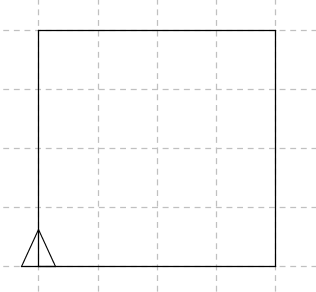
\includegraphics{bildoj/bases-carre.png}
\end{center}
\noindent Unu reta ^celo reprezentas 50 testudajn pa^sojn.  Por
desegni la apudan kvadraton, oni do tajpu:
\begin{verbatim}
an 200 dn 90 an 200 dn 90 an 200 dn 90 an 200 dn 90
\end{verbatim}
Oni rimarku ke oni ripetas $4$ fojojn la saman instrukcion, do jen
sintakso pli rapida:
\begin{verbatim}
ripetu 4 [an 200 dn 90]
\end{verbatim}
\subsection{La egallatera trilatero}
\begin{center}
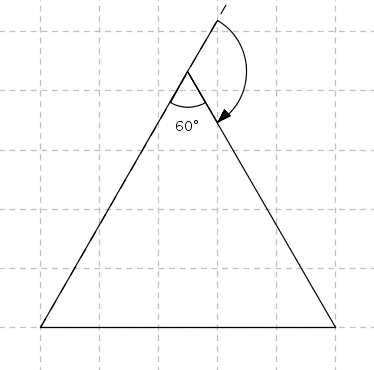
\includegraphics{bildoj/bases-triangle.png}
\end{center}
\noindent ^Ci tie, ^celo reprezentas 30 testudpa^sojn.  Ni vidos kiel
desegni tiun egallateran trilateron kun lateroj de 150 testudpa^soj.
La instrukcio similos ion tian:
\begin{verbatim}
ripetu 3 [an 150 dn ...]
\end{verbatim}
Restas kalkuli la bonan angulon.  En egallatera trilatero, l' anguloj
havas ^ciuj 60 gradojn.  ^Car la testudo turni^gas ekster la
trilatero, l' angulo validas $180-60=120$ gradojn.  L' instrukcio estas
do:
\begin{verbatim}
ripetu 3 [an 150 dn 120]
\end{verbatim}
\subsection{La seslatero}
\begin{center}
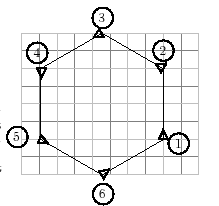
\includegraphics{bildoj/bases-hexagone.png}
\end{center}
\noindent ^Ci tie, ^celo reprezentas 20 testudpa^sojn.

\begin{verbatim}
ripetu 6 [an 80 dn ...]
\end{verbatim}

Oni rimarku ke dum ^gia movi^go, la testudo efektivigas kompletan
turni^gon (^gi ekiras adresita al supro, fine ^gi revenas en tiun
saman pozicion).  Tiu turni^go je 360 gradoj efektivi^gos post 6
eta^goj.  Tial, je ^ciu fojo, ^gi turni^gas je
${360} / {6}=60$\degre.

L' instrukcio estu do: \texttt{ripetu 6 [an 80 dn 60]}

\subsection{Desegni regulan plurlateron ^generale}
\noindent Efektive, ripetante la malgrandan pensadon anta^uan, oni
rimarku ke, por desegni plurlateron je $n$ lateroj, l' angulon oni
kalkulu per divido de $360$ per $n$.  Por ekzemplo:
\begin{itemize}
\item Por grafiki regulan kvinlateron je latero $100$:
\begin{verbatim}
ripetu 5 [an 100 dn 72]    (360:5=72)
\end{verbatim}
\item Por grafiki regulan na^ulateron je latero $20$:
\begin{verbatim}
ripetu 9 [an 20 dn 40]    (360:9=40)
\end{verbatim}
\item Por grafiki regulan ee... 360-lateron je latero $2$ (^gi ja
  similas cirklon!):
\begin{verbatim}
ripetu 360 [an 2 dn 1]  
\end{verbatim}
\item Por grafiki seplateron je latero $120$:
\begin{verbatim}
ripetu 7 [an 120 dn 360/7]
\end{verbatim}
\end{itemize}

\section{Registri proceduron}
\noindent Por ne devi retajpi ^ciufoje l' instrukciojn por desegni
kvadraton, trilateron... oni povas difini personajn komandojn nomatajn
\og proceduroj\fg.  Proceduro komenci^gas per la ^cefvorto
\texttt{por} kaj fini^gas per la ^cefvorto \texttt{fino}.  Oni
malfermu la redaktilon kaj tajpu ekzemple

\begin{verbatim}
por kvadrato
ripetu 4 [an 100 dn 90]
fino
\end{verbatim}

Poste oni fermu l' redaktilon registrante l' modifojn per klaki la
butonon testudo.  Nun je ^ciu fojo kiam oni tajpas \texttt{kvadrato},
kvadrato aperas sur l' ekrano!

\section{Ekzerco...}
\noindent
Malgranda reta ^celo reprezentas $10$ testudpa^sojn.

Provu realigi la grafikon malsupran per difini ok procedurojn:
\begin{itemize}
\item Proceduron \og \texttt{kvadrato}\fg{} kiu grafikos la bazan
  kvadraton de la domo.
\item Proceduron \og \texttt{tri}\fg{} kiu grafikos l' egallateran
  trilateron kiu reprezentos la tegmenton doman.
\item Proceduron \og \texttt{pordo}\fg{} kiu grafikos l' ortangulon
  reprezentantan la pordon.
\item Proceduron \og \texttt{kam}\fg{} kiu grafikos la kamentubon.
\item Proceduron \og \texttt{mov1}\fg{} kiu ebligos la testudon
  movi^gi de pozicio A al pozicio B.
\item Proceduron \og \texttt{mov2}\fg{} kiu ebligos la testudon
  movi^gi de pozicio B al pozicio C.
\item Proceduron \og \texttt{mov3}\fg{} kiu ebligos la testudon
  movi^gi de pozicio C al pozicio D.  (Atentu: eble necesos levi la
  testudan krajonon...)
\item Proceduron \og \texttt{domo}\fg{} kiu ebligos grafiki la domon
  tutan helpe de ^ciuj aliaj proceduroj.
\end{itemize}
\label{maison}
\begin{center}
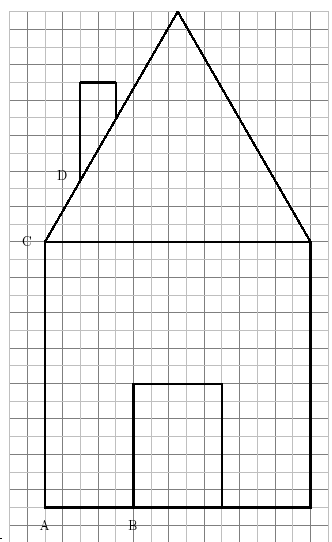
\includegraphics[scale=0.6]{bildoj/bases-maison.png}
\end{center}

\chapter{Uzi koordinatojn}
\label{koordinatoj}

{ }\hfill\textbf{Nivelo:} komencanto
\section{Prezentado}
\noindent En tiu ^ci ^capitro, ni malkovros la primitivon
\texttt{situon\_provizu}.  La desegnareo havas dratreton kies origino
estas lokita je la centro de la ekrano.  Oni povas atingi ^ciun
punkton de la desegnejo per helpo de ^giaj koordinatoj.

\texttt{sitp listo}\hspace {4cm } \textcolor{red}{ \texttt{sitp [100 -250]}}\\
Movas la testudon al la punkto kies koordinatojn difinas la listo.\\ \\
\\ Malgranda uzekzemplo:\\
\texttt{ev sitp [200 100] sitp [50 -150] sitp [-100 -150]}
\begin{center}
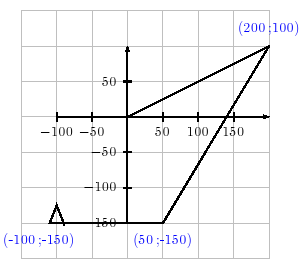
\includegraphics[scale=0.7]{bildoj/fpos-coord.png}
\end{center}
\vspace{1cm}
\section{Ekzerco:}
\noindent
Realigu tiun figuron nur uzante la primitivojn: \texttt{sitp}, \texttt{ev}, \texttt{l}, \texttt{ml}.\\
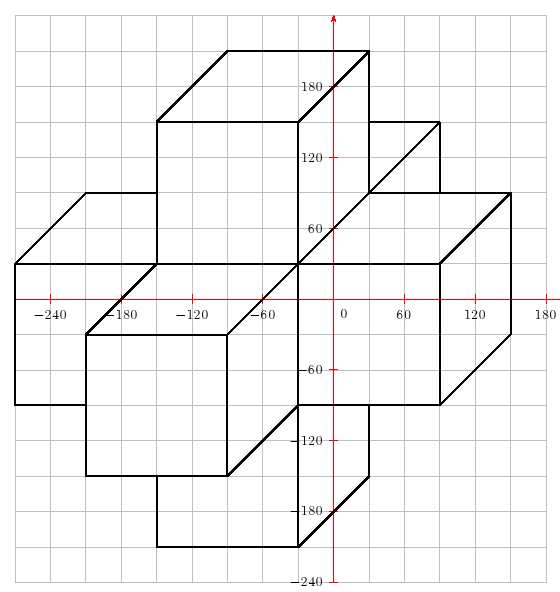
\includegraphics[scale=0.7]{bildoj/fpos-cube.png}

\chapter{La variabloj}
\label{variabloj}

{ }\hfill\textbf{Nivelo:} komencanto

\noindent \noindent Kelkafoje, oni deziras grafiki figuron je malsamaj
skaloj.  Por ekzemplo, se oni dezirus desegni kvadraton de latero 100,
kvadraton de latero 200 kaj kvadraton de latero 50, oni difinus tri
malsamajn procedurojn rilatajn al ^ciu kvadrato.
\begin{verbatim}
por kvadrato1
ripetu 4 [an 100 dn 90]
fino
por kvadrato2
ripetu 4 [an 200 dn 90]
fino
por kvadrato3
ripetu 4 [an 50 dn 90]
fino
\end{verbatim}

Oni rimarkas tuj ke estus pli simple, difini solan proceduron al kiu
oni dirus la ^gustan longon de la latero desegnota.  Ekzemple,
\texttt{kvadrato 200} grafikus la kvadraton de latero $200$,
\texttt{kvadrato 100} grafikus la kvadraton je latero $100$, ktp.  Ja
tion ebligos la variabloj.

\section{Uzekzemploj}
\noindent Por grafiki kvadraton je latero $100$, oni uzu:
\begin{verbatim}
por kvadrato
ripetu 4 [an 100 dn 90]
fino
\end{verbatim}
Ni modifos tiun proceduron por ke ^gi ricevu parametron (oni diras
egale \og argument\fg) indikantan la longon grafikotan.  Variabla nomo
^ciam estas anta^uata de la signo \og :\fg.  Kiam oni volas indiki ke
la proceduron \texttt{kvadrato} dependas je la variablo \texttt{:l}, oni
aldonu \texttt{:l} ^ce la fin' de la lini' de la difino.

Tiel, oni anta^ueniros ne plu $100$ testudpa^sojn, sed \texttt{:l}
testudpa^sojn.  La proceduro esti^gu:

\begin{verbatim}
por kvadrato :l
ripetu 4 [an :l dn 90]
fino
\end{verbatim}
Tiel, tajpante: \texttt{kvadrato 100 kvadrato 50 kvadrato 30 kvadrato 20 kvadrato 10}\\
 \begin{center}
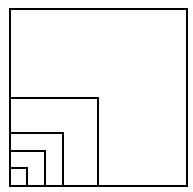
\includegraphics[scale=0.5]{bildoj/variables-carres.png}
\end{center}
\vspace{1cm}
\section{Grafiki ortangulon je longo kaj lar^go difinitaj}
\noindent Oni difinos ^ci tie proceduron nomatan \texttt{ort} kiu
dependu je du variabloj reprezentantaj la du dimensiojn de ortangulo.
\texttt{ort 200 100} grafikos ortangulon je alto $200$ kaj lar^go $100$.
\begin{verbatim}
por ort :lo :la
ripetu 2 [an :lo dn 90 an :la dn 90]
fino
\end{verbatim} 
Faru provojn:
\begin{verbatim}
ort 200 100 ort 100 300 ort 50 150 ort 1 20 ort 100 2 
\end{verbatim}
Kompreneble, se vi donas nur unu argumenton al la proceduro
\texttt{ort}, l' interpretilo signalos per erarmesa^go ke la proceduro
atendas alian argumenton.
\section{Grafiki formon je malsamaj ampleksoj}
\noindent
Ni jam vidis kiel grafiki kvadraton, ortangulon je malsamaj ampleksoj.
Ni reprenos l' ekzemplon de la domo de p.~\pageref{maison} kaj vidos
kiel modifi la kodon por grafiki la domon je la dezirata skalo.

La celo estas pasigi argumenton al proceduro \texttt{domo} por ke la^u
la parametro, la domo estu pli a^u malpli granda.  Ni deziras ke 
\texttt{domo 1} grafiku la domon je reala amplekso.

\texttt{domo 0.5} grafikos domon je skalo $0.5$.

\texttt{domo 2} grafikos domon je dimensioj duoblaj, ktp.

La koncepto proporcieco estas kompreneble subka^sita.  En reala
grando, la proceduro \texttt{kvadrato} estis jena:
\begin{verbatim}
por kvadrato
ripetu 4 [an 150 dn 90]
fino
\end{verbatim}
^Ciuj originalaj diminsioj de la domo estas multiplikitaj per la
skalo.  La proceduro \texttt{kvadrato} esti^gas:
\begin{verbatim}
por kvadrato :l
ripetu 4 [an 150*:l dn 90]
fino
\end{verbatim}
Do kiam oni tajpos \texttt{kvadrato 2}, la kvadrato havos lateron
longan je $150\times2=300$.  La proporciojn oni respektos!  Efektive,
oni rimarku ke necesos repreni ^ciujn procedurojn kaj ^san^gi la
longojn je movo la^u la jena maniero:

\texttt{an 70} fari^gos \texttt{an 70*:l}

\texttt{an 45} fari^gos \texttt{an 45*:l}

ktp.

\begin{verbatim}
por kvadrato :l
ripetu 4 [an 150*:l dn 90]
fino

por tri :l
ripetu 3[an 150*:l dn 120]
fino

por pordo :l
ripetu 2 [an 70*:l dn 90 an 50*:l dn 90]
fino

por kam :l
an 55*:l dn 90 an 20*:l dn 90 an 20*:l
fino

por mov1 :l
dn 90 an 50*:l mdn 90
fino

por mov2 :l
mdn 90 an 50*:l dn 90 an 150*:l dn 30
fino

por mov3 :l
l dn 60 an 20*:l mdn 90 an 35*:l ml
fino

por dom :l
kvadrato :l mov1 :l pordo :l mov2 :l tri :l mov3 :l kam :l
fino
\end{verbatim}

\section{Ekzerco:}
\noindent Realigu la desegnojn jenajn per variabloj tiel ke oni povas
obteni ilin je diversaj ampleksoj.

\begin{center}
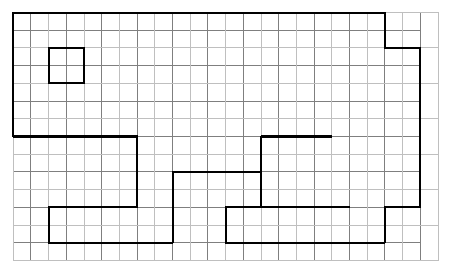
\includegraphics[scale=0.7]{bildoj/variables-grenouille.png}
\end{center}
\begin{center}
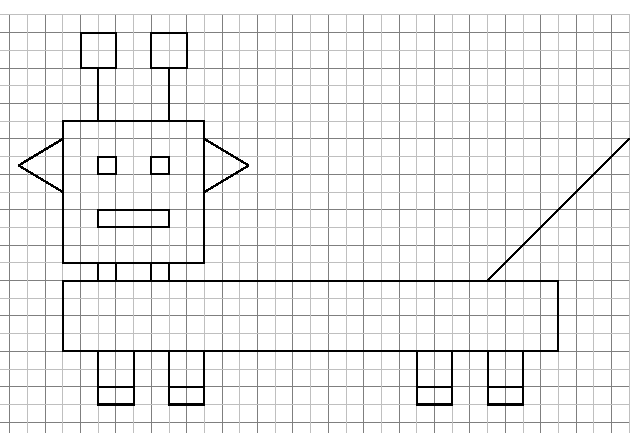
\includegraphics[scale=0.75]{bildoj/variables-robot.png}
\end{center}

\chapter{La rekursiveco}
{ }\hfill\textbf{Nivelo:} meza

\noindent  La lingvo Logo uzas tre ofte te^hnikon programadan nomatan
rekursiveco.  En ^ci tiu ^capitro, ni malkovros tuj tiun koncepton per
simplaj ekzemploj por poste profundi^gi per ^cefe la desegnado de
fraktalo nomata la ne^gero de Van Koch.  Por komenci, jen malgranda klarigo:
\begin{center}
\textbf{Proceduro estas rukursivo se ^gi vokas sin mem.}
\end{center}
\section{En desegnejo}
\subsection{Unua ekzemplo}
\begin{verbatim}
por ekz1
dn 1
ekz1
fino  
\end{verbatim}
Tiu proceduro estas rekursiva ^car la proceduro \texttt{ekz1} estas
vokata je la lasta linio.  Dum la rulado, oni konstatas ke la testudo
ne ^cesas turni^gi.  Por haltigi la programon, oni nepre premu la
butonon STOP.
\subsection{Dua ekzemplo}
\noindent Anta^u ^cio, jen tri novaj primitivoj:
\begin{itemize}
\item [$\bullet$] \texttt{atendu nombro}\hspace {4cm } \textcolor{red}{ \texttt{atendu 60}}\\
Haltigu la programon dum tiom da 60$^{\textrm{onoj}}$ de sekundo kiel indikite. \\
Ekzemple, \texttt{atendu 120} haltigos la programon dum du sekundoj.
\item [$\bullet$] \texttt{gum,gumskrapu}\hspace {4cm } \textcolor{red}{{gumskrapu}}\\
Kiam la testudo movi^gas, ^gi forvi^sas anstata^u skribi post si.
\item [$\bullet$] \texttt{desegne}\hspace {4cm } \textcolor{red}{{desegne}}\\
Metu la testudon en la moduson de klasika desegno: la testudo skribas post si dum movi^gi.
\end{itemize}
\noindent
\begin{verbatim}
por ekz2
an 200 gum atendu 60
man 200 desegne dn 6
ekz2
fino
\end{verbatim}
Nur restas ruli tiun programon.  Je ^ciu sekundo la sama motivo
rekomenci^gas kaj la programo ^sajnigas sekundhorlo^gon!
\section{En tekstejo}
\subsection{Unua ekzemplo}
\noindent La primitivo \texttt{skribu, s} ebligas skribi tekston en la
tekstareon.  ^Gi atendas kiel argumenton jen liston, jen vorton.  Ekz.:
\texttt{s "saluton} \texttt{s [Mi skribas kion mi volas]}.  (Ne
forgesu la citilon " kiam oni volas skribi nur vorton.)
\begin{verbatim}
por ekz3 :n
skribu :n
ekz3 :n+1
fino
\end{verbatim}
Rulu la komandon \texttt{ekz3 0}, poste haltigu per butono STOP.
Faru la ^san^gojn necesajn en tiu programo por ke la numeroj aperu duope.

Nun mi volas skribi ^ciun nombron pli grandan ol $100$ kiu estas en la
multipliktabelo de la kvino.  Sufi^cas do modifi la programon jene:
\begin{verbatim}
por ekz3 :n
skribu :n
ekz3 :n+5
fino
\end{verbatim}
kaj ruli: \texttt{ekz3 100}
\subsection{Realigi eliran provon}
\noindent Tajpu la jenajn komandojn:\\
\texttt{se 2+1=3 [skribu [tio estas vera]]} \\
\texttt{se 2+1=4 [skribu [tio estas vera]] [skribu [la kalkulo estas malvera]]} \\
\texttt{se 2+5=7 [s "vera] [s "malvera]}\\
\\
Se vi ankora^u ne komprenas la sintakson de la primitivo \texttt{se},
adresi^gu al la referenca gvidlibro \xlogo.
\begin{verbatim}
por ekz3 :n
se :n=100 [haltu]
skribu :n
ekz3 :n+1
fino
\end{verbatim}

Rulu la komandon \texttt{ekz3 0}

Faru la ^san^gojn necesajn en tiu programo por aperigi la nombrojn
ku^santaj inter $55$ kaj $350$ kiu estas en la multipliktabelo de la
dek-unuo.

\section{Ekzemplo de fraktalo: la ne^gero de Koch}

Danke al la rekursiveco, tre facilas generi en \logo\ objektojn
nomatajn en matematiko \emph{fraktaloj}.

Jen la unuaj stadioj ebligantaj krei la malglatan linion de Van Koch.
\begin{center}
  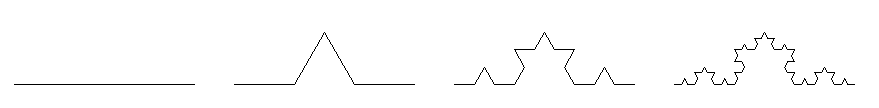
\includegraphics[width=\textwidth]{bildoj/koch0123.png}
\end{center}
En ^ciu stadio:
\begin{enumerate}
\item ^Ciu segmento estu partigita en tri egalajn partojn.
\item Oni grafiku egallateran trilateron sur la dua segmento.
\item Oni forigu tiun duan segmenton.
\end{enumerate}
\textbf{Rimarkenda:} Konsiduru la duan stadion; konstatu ke tiun
linion formas kvar motivoj rilataj al l' anta^ua stadio kaj kies
amplekso estas triono.  Tiel evidenti^gas la rekursiva naturo de la
fraktalo.

Nomu $L_{n,\ell}$ la motivon longa je $\ell$, grafikita en la stadio $n$.
Por grafiki tiun motivon jen la procedo:
\begin{enumerate}
 \item Desegnu $L_{n-1,\ell/3}$
 \item Turnu maldekstren je $60$ gradoj
 \item Desegnu $L_{n-1,\ell/3}$
 \item Turnu dekstren je $120$ gradoj.
 \item Desegnu $L_{n-1,\ell/3}$
 \item Turnu maldekstren je $60$ gradoj
 \item Desegnu $L_{n-1,\ell/3}$
\end{enumerate}
En \logo, tio fari^gas tutsimple:
\begin{verbatim}
# :l longo de la motivo 
# :p stadio
por linio :l :p
se :p=0 [an :l] 
  [linio :l/3 :p-1 dn 60 linio :l/3 :p-1 dn 120 linio :l/3 :p-1 dn 60 linio :l/3 :p-1]
fino
\end{verbatim}
Se oni desegnas egallateran trilateron konsistanta el tri tiaj linioj,
oni akiras mirindan ne^geron de Van Koch
\begin{verbatim}
# :l longo de la latero
por neĝero :l :p
ripetu 3 [linio :l :p dn 120]
fino
\end{verbatim}
Poste rulu: \texttt{flocon 200 6}
\begin{center}
  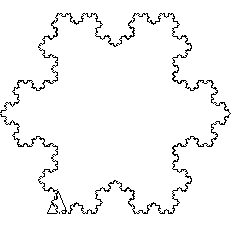
\includegraphics{bildoj/flocon.png}
\end{center}
\section{Rekursiveco pri vortoj}
Priser^cu la liston de primitivoj je p.\,\pageref{liste-prim} por
kompreni la rolon de la primitivoj \texttt{vort}, \texttt{lastan}, kaj
\texttt{senlastan}.

Jen rekursiva proceduro kiu ebligas renversi l' ordon de la literoj de
vorto.
\begin{verbatim}
por renversuv :v
se malplena? :v [sendu "]  
sendu vorton lastan :v renversuv senlastan :v
fino

skribu renversuv "abcĉde
edĉcba
\end{verbatim}
Oni diras ke vort' estas palindromo se oni povas legi ^gin je amba^u
direktoj (ekzemploj: ama, radar', onano...).
\begin{verbatim}
# testu ĉu la vorto :v estas palindromo
por palindromo :m
se  :m = renversuv :m [sendu vera] [sendu malvera] 
fino
\end{verbatim}
Kaj finfine jen mojosa programeto (dankon Olivier SC):
\begin{verbatim}
por palin :n
se palindromo :n [skribu :n haltu]
skribu (list :n "PLUS renversuv :n "EGALAS sumon :n renversuv :n)
palin :n + renversuv :n 
fino

palin 78
78 PLUS 87 EGALAS 165
165 PLUS 561 EGALAS 726
726 PLUS 627 EGALAS 1353
1353 PLUS 3531 EGALAS 4884
4884
\end{verbatim}
\section{Kalkuli faktorialon}
\label{factorielle}
Oni difinas faktorialon de $5$, indikite $5!$ jene:
 $$5!=5\times4\times3\times2\times1=120$$
^Generale, por $n$ strikte pozitiva, rimarku ke: $n!=n\times(n-1)!$.
Tiu rilato klarigas la rekursivan naturon de jena programo:
\begin{verbatim}
por fak :n
se :n=0 [snd 1] [snd :n * fak :n-1]
fino

s fak 5
120
s fak 6
720
\end{verbatim} 
 \section{Proksimumo de $\pi$}
\label{approx-pi}
Oni povas akiri proksimumon de la nombro $\pi$ per la formulo:
$$\pi\approx2^k\sqrt{2-\sqrt{2+\sqrt{2+\ldots\sqrt{2+\sqrt2}}}}$$ 
kie $k$ estas la nombro de kvadrataj radikoj.  Ju pli granda estas $k$
des pli tiu esprimo proksimi^gas al nombro $\pi$.

La formulo konsistas el la esprimo $2+\sqrt{2+\ldots\sqrt{2+\sqrt2}}$
kiu estas klare rekursiva, de kie la programo jena:
\begin{verbatim}
# k estas la nombro de radikoj
por aprokspi :k
tajpu "Proksimume:\  s (potencon 2 :k) * radikon (2 - radikon (kalk :k-2))
s "-------------------------
tajpu "Pi:\  s pi
fino

por kalk :p
se :p=0 [snd 2] [snd 2 + racine kalk :p-1]
fino

aprokspi 10
Proksimume: 3.141591421568446 
------------------------- 
Pi: 3.141592653589793 
\end{verbatim}
Oni akiris la $5$ unuajn decimalojn!  Se oni deziras pli, necesos
forigi kelkajn kalkulerarojn pro ne precize kalkuli la koncernitajn
kvadrataj radikojn.  Por tio ni pligrandigos la nombron de decimaloj
per la primitivo \texttt{decimalojn\_provizu}.
\begin{verbatim}
decimalojn_provizu 100
aprokspi 100
Proksimume: 3.1415926535897932384626433832795028841973393069670160975807684313880468...
------------------------- 
Pi: 3.141592653589793238462643383279502884197169399375105820974944592307816406....
\end{verbatim}
Kaj nun oni akiras 39 decimalojn...

\chapter{Krei movadon}
{ }\hfill\textbf{Nivelo:} meza

^Ci tiu ^capitro proponas du aferojn tre malsamajn kies celo estas krei
movadon per \xlogo.

\section{La ciferoj de la kalkulilo}

\begin{center}
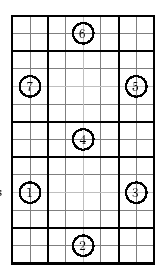
\includegraphics{bildoj/animation-chiffre.png}
\end{center}

^Ci tiu tasko bazi^gas sur la fakto ke ^ciun kalkulilan nombron oni
povas akiri per la jena ^sablono:
\begin{itemize}
\item Por ekzemplo, por desegni \og 4\fg, oni ^saltu l' ortangulojn 3, 4, 5, 7.
\item Por desegni \og 8\fg, oni ^saltu l' ortangulojn 1, 2, 3, 4, 5, 6, 7.
\item Por desegni \og 3\fg, oni ^saltu l' ortangulojn 2, 3, 4, 5, 6.
\end{itemize}

\subsection{Plenigi ortangulon}
\begin{center}
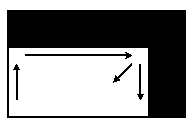
\includegraphics{bildoj/animation-rectangle.png}
\end{center}
Se oni deziras ekzemple grafiki plenan ortangulon grandan je $100$ mul
$200$, unua ideo povas esti desegni la ortangulon je $100$ mul $200$,
poste desegni ortangulon je $99$ mul $199$, poste ortangulon je $98$
mul $198$... ^gis la ortangul' estos tute plena.

Ni komencu per difini ortangulon je lango kaj lar^go dependaj je du
variabloj.
\begin{verbatim}
por ort :lo :la
ripetu 2 [an :lo dn 90 an :la dn 90]
fino
\end{verbatim}
Por plenigi nian grandan ortangulon, oni rulu:

\texttt{ort 100 200 ort 99 199 ort 98 198  ..... ort 1 101}

Difinu tiam proceduron ortangulo dedi^cita grafiki tiun plenan ortangulon.
\begin{verbatim}
por ortangulo :lo :la
ort :lo :la
ortangulo :lo-1 :la-1
fino
\end{verbatim}
Oni provu \texttt{ortangulo 100 200} kaj oni rimarku ke estas
problemo: la proceduro ne haltas kiam la ortangulo estas plena; ^gi
plu grafikas ortangulojn!  Oni do aldonu provon ebligantan detekti ^cu
la longo a^u la lar^go egalas $0$.  Tiam, oni petas la programon halti
per la komando \texttt{haltu}.
\begin{verbatim}
por ortangulo :lo :la
se aŭ :lo=0 :la=0 [haltu]
ort :lo :la
ortangulo :lo-1 :la-1
fino
\end{verbatim}
Rimarko: anstata^u uzi la primitivon \texttt{a^u}, oni povas uzi la
simbolon \og|\fg; oni skribus:
\begin{center}
\texttt{se :lo=0 | :la=0 [haltu]}
\end{center}

\subsection{La programo}
\noindent Ni bezonas la plenan ortangulon anta^uan:
\begin{verbatim}
por ort :lo :la
se :lo=0 |:la=0 [haltu]
ripetu 2 [an :lo dn 90 an :la dn 90]
ort :lo-1 :la-1
fino
\end{verbatim}

Ni supozas ke la testudo ekiras de la malsupra maldekstra angulo.  Ni
difinos proceduron nomatan \texttt{cifero} akceptantan $7$ argumentojn
\texttt{:a}, \texttt{:b}, \texttt{:c}, \texttt{:d}, \texttt{:e},
\texttt{:f}, \texttt{:g}.  Kiam \texttt{:a} valoras $1$, oni desegnu
la ortangulon $1$.  Se \texttt{:a} valoras $0$, oni ne desegnu ^gin.
Jen la principo.

Jen la proceduro:
\begin{verbatim}
por cifero :a :b :c :d :e :f :g
# Oni desegnu la ortangulon 1
se :a=1 [ort 160 40]
# Oni desegnu la ortangulon 2
se :b=1 [ort 40 160]
l dn 90 an 120 mdn 90 ml
# Oni desegnu la ortangulon 3
se :c=1 [ort 160 40]
l an 120 ml
# Oni desegnu la ortangulon 5
se :e=1 [ort 160 40]
# Oni desegnu la ortangulon 4
mdn 90 l man 40 ml
se :d=1 [ort 160 40]
# Oni desegnu la ortangulon 6
dn 90 l an 120 mdn 90 ml
se :f=1 [ort 160 40]
# Oni desegnu la ortangulon 7
l an 120 mdn 90 man 40 ml
se :g=1 [ort 160 40]
fino
\end{verbatim}
\subsection{Krei malgradan animadon}
^Ci tie ni simulos retronombradon aperigante sekvence la ciferojn de
$9$ ^gis $0$ je ordo malkreska.
\begin{verbatim}
por retronombro
ev tdk cifero 0 1 1 1 1 1 1 atendu 60
ev tdk cifero 1 1 1 1 1 1 1 atendu 60
ev tdk cifero 0 0 1 0 1 1 0 atendu 60
ev tdk cifero 1 1 1 1 0 1 1 atendu 60
ev tdk cifero 0 1 1 1 0 1 1 atendu 60
ev tdk cifero 0 0 1 1 1 0 1 atendu 60
ev tdk cifero 0 1 1 1 1 1 0 atendu 60
ev tdk cifero 1 1 0 1 1 1 0 atendu 60
ev tdk cifero 0 0 1 0 1 0 0 atendu 60
ev tdk cifero 1 1 1 0 1 1 1 atendu 60
fino
\end{verbatim}

Jen malgranda problemo: estas palpebruma efiko malagraba dum krei
^ciun ciferon.  Por fluemigi tion oni uzos la primitivojn
\texttt{movado}, \texttt{neplu\_movigu} kaj \texttt{novigu}.
\begin{itemize}
\item \texttt{movado} ebligas ^salti la moduson \og movado\fg.  La
  testudo ne desegnos plu sur l' ekrano, sed en bufro, tio estas, en
  memoro.  ^Gi aldonos la bildon nur kiam oni petos per la primitivo
  \texttt{novigu}.
\item \texttt{neplu\_movigu} ebligas mal^salti tiun moduson kaj reveni
  en la klasikan moduson.
\end{itemize}
Jen la modifita programo:
\begin{verbatim}
por retronombro
# Pasu en moduson movado
movado
ev tdk cifero 0 1 1 1 1 1 1 novigu atendu 60
ev tdk cifero 1 1 1 1 1 1 1 novigu atendu 60
ev tdk cifero 0 0 1 0 1 1 0 novigu atendu 60
ev tdk cifero 1 1 1 1 0 1 1 novigu atendu 60
ev tdk cifero 0 1 1 1 0 1 1 novigu atendu 60
ev tdk cifero 0 0 1 1 1 0 1 novigu atendu 60
ev tdk cifero 0 1 1 1 1 1 0 novigu atendu 60
ev tdk cifero 1 1 0 1 1 1 0 novigu atendu 60
ev tdk cifero 0 0 1 0 1 0 0 novigu atendu 60
ev tdk cifero 1 1 1 0 1 1 1 novigu atendu 60
# Revenu en moduson klasikan
neplu_movigu
fino
\end{verbatim}

\section{Animado: la hometo kiu kreskas}
\begin{center}
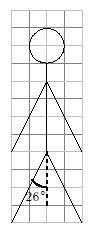
\includegraphics{bildoj/animation-bonhomme.png}
\end{center}
Anta^u ^cio, ni difinu proceduron \texttt{hometo} kiu grafikas la
hometon apudan je elektita amplekso.
\begin{verbatim}
por hometo :c
mdn 154 an 44*:c man 44*:c 
mdn  52 an 44*:c man 44*:c 
mdn 154 an 40*:c
mdn 154 an 44*:c man :c*44 
mdn  52 an 44*:c man :c*44 
mdn 154 an 10*:c
mdn  90 ripetu 180 [an :c/2 dn 2] dn 90
fino
\end{verbatim}
Nun ni kreos animadon ^sajnigantan ke la hometon kreskas po malmulte.
Por tio, ni grafikos \texttt{hometo 0.1}, poste \texttt{hometo 0.2},
\texttt{hometo 0.3}... ^gis \texttt{hometo 5}.  Inter ^ciu grafikado,
oni forvi^sos l' ekranon.  Jen la du proceduroj:
\begin{verbatim}
por hometo :c
mdn 154 an 44*:c man 44*:c 
mdn  52 an 44*:c man 44*:c 
mdn 154 an 40*:c
mdn 154 an 44*:c man :c*44 
mdn  52 an 44*:c man :c*44 
mdn 154 an 10*:c
mdn  90 ripetu 180 [an :c/2 dn 2] dn 90
se :c=5 [haltu]
ev tdk hometon :c+0.1
fino

por komenci
ev tdk
hometo 0
fino
\end{verbatim}
Finfine, por fluemigi la tuton, oni helpu sin per la moduson movado kaj la primitivo \texttt{novigu}.
\begin{verbatim}
por hometo :c
mdn 154 an 44*:c man 44*:c 
mdn  52 an 44*:c man 44*:c 
mdn 154 an 40*:c
mdn 154 an 44*:c man :c*44 
mdn  52 an 44*:c man :c*44 
mdn 154 an 10*:c
mdn  90 ripetu 180 [an :c/2 dn 2] dn 90
novigu
se :c=5 [haltu]
ev tdk hometo :c+0.1
fino

por komenci
tdk movado
hometo 0
neplu_movigu
fino

\end{verbatim}
\textbf{Rimarku: } Tie, la proceduro \texttt{hometo} estas rekurziva;
oni pli simple povus uzi la primitivon \texttt{ripetupor} por variigi
\texttt{:c} de $0.1$ ^gis $5$.  Jen la programo tiel:
\begin{verbatim}
por hometo :c
ev tdk mdn 154 an 44*:c man 44*:c 
mdn  52 an 44*:c man 44*:c 
mdn 154 an 40*:c
mdn 154 an 44*:c man :c*44 
mdn  52 an 44*:c man :c*44 
mdn 154 an 10*:c
mdn  90 ripetu 180 [an :c/2 dn 2] dn 90
novigu
fino

por komenci
tdk movado
ripetupor [c 0 5 0.1] [hometo :c]
neplu_movigu
fino

\end{verbatim}


\chapter{Interaktiva programado}
\label{interaktiva}

{ }\hfill\textbf{Nivelo:} komencanto
\section{Komuniki kun l' uzulo}

Ni realigos malgrandan programon kiu demandas de l' uzulo ^slian
nomon, baptonomon kaj a^gon.  Je l' fin' de la demandaro, la programo
respondos per memorigilo jene:
\begin{verbatim}
Via familinomo estas:........
Via baptonomo estas: .......
Via aĝo estas: .......
Vi estas (mal)plenkreskulo
\end{verbatim}
\textsc{Por tio, ni uzos la jenajn primitivojn:}
\begin{itemize}
\item \texttt{legu}:\hspace{4cm}  \textcolor{red}{ \texttt{legu [Kiom estas via a^go? ] "a}}

  Aperigas dialogfenestron kun titolo kiel la listo argumento (tie,
  \og Kiom estas via a^go?\fg). La respondo donita de l' uzulo estas
  memorita kiel vorto a^u listo (se l' uzul' tajpas plurajn
  vortojn) en la variablo \texttt{:a}.

\item \texttt{provizu, p}:\hspace{4cm}  \textcolor{red}{ \texttt{provizu "a 30}}

  Donas la valoron $30$ al la variablo \texttt{:a}

\item \texttt{frazon, fr}:\hspace{4cm}  \textcolor{red}{ \texttt{frazon [30 k] "a }}

  Aldonas valoron en liston.  Se tiu valoro estas listo, kunigas la du listojn.

\begin{verbatim}
frazon [30 k] "a ---> [30 k a]
frazon [1 2 3] 4 ---> [1 2 3 4]
frazon [1 2 3] [4 5 6] ---> [1 2 3 4 5 6]
\end{verbatim} 
\end{itemize}
Jen la kodo:
\begin{verbatim}
por demandaro
legu [Kiom aĝas vi?] "aĝo
legu [Kio estas via familinomo?] "famnomo
legu [Kio estas via baptonmo?] "bapnomo
skribu frazon [Via familinomo estas: ] :famnom
skribu frazon [Via baptonomo: ] :bapnomo
skribu frazon [Via aĝo estas: ] :aĝo
se aŭ :aĝo>18 :aĝo=18 [skribu [Vi estas plenkreskulo]] [skribu [Vi estas malplenkreskulo]]
fino
\end{verbatim}

\section{Programi malgrandan ludon}

\textsc{La celo de ^ci tiu sekcio estas krei la jenan ludon:}

La programo elektas hazardan nombron inter $0$ kaj $32$ kaj memoras
^gin.  Dialogfenestro aperas kaj demandas l' uzulon enigi nombron.  Se
la proponita nomo estas egala al la memorita nomo, ^gi skribas \og
venkis\fg en la tekstejo.  En mala okazo, la programo indikas ^cu la
nombro memorita estas pli malgranda a^u granda ol la nombro proponita
de l' uzulo; poste ^gi reaperigas la dialogfenestron.  La programo
haltos kiam l' uzulo trovas la memoritan nombron.

Vi bezonos uzi la jenan primitivon:

\texttt{hazardon, hzd}: \hspace{4cm} \textcolor{red}{\texttt{hazardon 8}} 

\texttt{hazardon 20} donas nombron hazarde elektitan inter $0$ kaj $19$.

\textsc{Jen kelkaj reguloj respektendaj por realigi tiun ludon:}
\begin{itemize}
\item La nombro memorita de l' komputilo estas memorata en variablo
  nomata \texttt{nombro}.
\item La dialogfenestro havos por titolo; \og Proponu nombron:\fg.
\item La nombro proponita de l' uzulo estos registrita en variablo
  nomata \texttt{provo}.
\item La proceduro kiu ebligas ruli la ludon nomi^gos  \texttt{ludo}.
\end{itemize}

\vspace{0.5cm}
\textsc{Kelkaj eblaj plibonigoj:}
\begin{itemize}
\item Skribi la nombro de provoj.
\item La nombro ser^cota estu inter $0$ kaj $2000$.
\item Konstati ^cu tio enigita de l' uzulo estas vere nombro.  Por
  tio, uzu la primitivon \texttt{nombra?}.

  Exemples: \begin{tabular}[t]{l}
    \texttt{nombra? 8} estas vera.\\
    \texttt{nombra? [5 6 7]} estas malvera ([5 6 7] estas listo sed ne
    nombro).\\
    \texttt{nombra? "abcde} estas malvera ("abcde estas
    vorto sed ne nombro).
\end{tabular}
\end{itemize}

\chapter{Temo: Sumi du kubojn}
{ }\hfill\textbf{Nivelo:} Meza

Kiam oni ^jetas du kubojn kaj kalkulas la tuton de poentoj de amba^u
kuboj, oni akiras entjeron inter $2$ kaj $12$.  ^Ci tie, ni vidos la
distribuon de la diversaj rezultoj kaj ^gin reprezentos per malgranda
grafiko.

\section{Simuli ^jeti kubon}
Por simuli ^jeton de kubo, ni uzos la primitivon \texttt{hazardon}.  Jen kiel procedi.

\texttt{hazardon 6} $\longrightarrow$ redonas entjeron hazarde
elektitan el $0$, $1$, $2$, $3$, $4$, $5$.

Tial, \texttt{(hazardon 6) + 1} redonas entjeron elektitan el $1$,
$2$, $3$, $4$, $5$, $6$.  Rimarku ja la parentezojn; alie l'
interpretilo Logo komprenus \texttt{hazardon 7}.  Por ^spari l'
parentezojn, oni povas tajpi \texttt{1 + hazardon 6}.

Oni difinu tiel la proceduron \texttt{^jetu} kiu simulas ^jeti
ludkubon.
\begin{verbatim}
 por ĵetu
   sendu 1 + hazardon 6
 fino
\end{verbatim}
 \section{La programo}
 Ni uzos la moduson plur-testudan.  Por tiel havi plurajn testudojn
 sur l' ekran', oni uzu la primitivon \texttt{testudon\_provizu}
 sekvitan de la numero de la testudo kiun oni volas elekti.

 Bona skemo valoras pli ol mil klarigoj...
\begin{center}
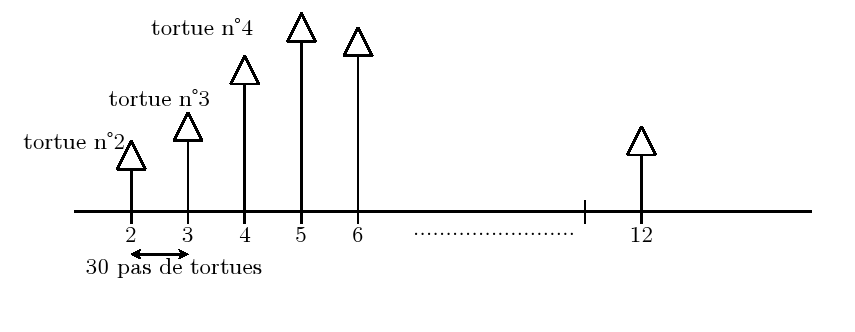
\includegraphics[scale=0.45]{bildoj/somme-des-schema.png}
\end{center}
\vspace{0.5cm} ^Ciu testudo numerata de $2$ ^gis $12$ anta^ueniros unu
testudpa^son kiam la sumo de la du kuboj ^jetitaj estas egala a ^gia
numero.  Por ekzemplo, se la kubo sumi^gas $8$, la testudo $8$a
anta^ueniru unu pa^son.  Inter ^ciuj du testudoj estu $30$
testudpa^soj horizontale.

Oni lokos la testudojn per koordinatoj.
\begin{itemize}
 \item  La testudo n\degre2 estu lokita en $(-150;0)$
 \item  La testudo n\degre3 estu lokita en $(-120;0)$
 \item  La testudo n\degre4 estu lokita en $(-90;0)$
 \item  La testudo n\degre5 estu lokita en $(-60;0)$\\
\begin{minipage}{8 cm}
\begin{center}
 $\vdots$
\end{center}
\end{minipage}
\end{itemize}
\begin{verbatim}
 testudon_provizu 2 sitp [-150 0]
 testudon_provizu 3 sitp [-120 0]
 testudon_provizu 4 sitp  [-90 0]
 testudon_provizu 5 sitp  [-60 0]
 testudon_provizu 6 sitp  [-30 0]
.....
\end{verbatim}
Pli bone ol tajpi $11$ fojojn preska^u la saman komandlinion, oni
a^utomatigu tion uzante la primitivon \texttt{ripetupor}.  Per tiu
primitivo, oni povas havigi al variablo sekvencon de valoroj prenitaj
en intervalo la^u samaj spacoj.  ^Ci tie, oni volas ke la variablo
\texttt{:i} prenu sinsekve la valorojn $2$, $3$, $4$... $12$.  Oni
tajpu:

\texttt{ripetu por [i 2 12] [ listo de rulotaj instrukcioj ]}

Por loki la testudojn, oni kreu do la proceduron \texttt{pretigu}
\begin{verbatim}
por pretigu
  ev tdk
  ripetupor [i 2 12]  
      [# Loku la testudon
       testudon_provizu :i sitp liston -150+(:i-2)*30 0
       # Skribu la numeron de la testudo apude sube
       l man 15 etikedu :i an 15 ml]
fino
\end{verbatim}

Bone komprenu la formulon \texttt{-150+(:i-2)*30}.  Oni ekiras de
$-150$; poste por ^ciu nova testudo oni aldonas $30$.  Provu per la
diversaj valoroj de \texttt{:i} se vi ne estas konvinkita.

Finfine jen la programo:
\begin{verbatim}
por ĵeti
 sendu 1 + hazardon 6
fino

por pretiu
  ev tdk
  ripetupor [i 2 12]  
      [# Loku la testudon
       testudon_provizu :i sitp liston -150+(:i-2)*30 0
       # Skribu la numeron de la testudo apude sube
       l man 15 etikedu :i an 15 ml]
fino

por startu
pretigu
# Realigu 1000 provoj
ripetu 1000 
  [provizu "sumo ĵetu+ĵetu
   testudon_provizu :sumo an 1]
# Skribu la frekvencojn de la ĵetado
ripetupor [i 2 12] 
 [testudon_provizu :i
  # L' ordinato de l' testudo reprezentas la nombron de ĵetoj
  loke_provizu "efika lastan sit 
  l an 10 mdn 90 an 10 dn 90 ml etikedu :efika/1000*100]
fino
\end{verbatim}

Jen ^generaligo de tiu programo.  Oni demandos al l' uzulo la nombron
de deziratajn kubojn kaj la nombron de ^jetojn farotajn.
\begin{verbatim}
por ĵetu
lokp "sumo 0
ripetu :kuboj 
  [lokp "sumo :sumo + 1 + hazardon 6]
sendu :sumo
fino

por pretigu
  ev tdk testudkiomon_provizu :maks+1
  ripetupor fr list "i :min :maks 
     [# Loku la testudon
      testudon_provizu :i sitp list (:min-:maks)/2*30+(:i-:min)*30 0
      # Skribu la numeron de la testudo apude sube
      l man 15 etikedu :i an 15 ml]
fino

por startu
leg [Nombro de kuboj:] "kuboj
se ne nombra? :kuboj [s [La nombro enigita ne estas valida!] haltu]
provizu "min :kuboj
provizu "maks 6*:kuboj
leg [Nombro de ĵetoj realigotaj] "ĵetoj
se ne nombra? :ĵetoj [s [La nombro enigita ne estas valida!] haltu]
pretigu
# Realigu 1000 provoj
ripetu :ĵetoj 
  [testudon_provizu ĵetu an 1]
# Ŝkribu la frekvencojn de la ĵetoj
ripetupor fr list "i :min :maks 
  [testudon_provizu :i
   # L' ordinato de l' testudo reprezentas la nombron de ĵetoj
   lokp "efika lastan sit 
   # Oni proksimumu je 0.1
   l an 10 mdn 90 an 10 dn 90 ml etikedu (entjeran :efika/:ĵetoj*1000) / 10]
fino

\end{verbatim}

\chapter{Temo: Proksimumi probablike al $\pi$}

{ }\hfill\textbf{Nivelo:} Alta

\textsc{Averto:} Necesas kelkaj nocioj pri matematiko por bone
kompreni ^ci tiun ^capitron.

\section{Nocio de pgkd (plej granda komuna dividanto)}

Donitaj du entjeroj, ilia pgkd estas la plej granda el la dividantoj
de amba^u.
\begin{itemize}
\item Por ekzemplo, $42$ kaj $28$ havas kiel pgkd $14$ (^gi dividas
  samtempe al $28$ kaj al $42$, kaj ^gi estas la plej granda el la
  nombroj tiaj).
\item $25$ kaj $55$ havas kiel pgkd $5$.
\item $42$ kaj $23$ havas kiel pgkd $1$.
\end{itemize}
Kiam du nombroj havas $1$ kiel pgkd, oni nomas ilin \emph{primoj inter
  si}.  Do por l' anta^ua ekzemplo, $42$ kaj $23$ estas primoj inter
si.  Tio signifas ke ili havas neniun komunan dividanton krom $1$
(kompreneble, ^gi dividas ^ciun entjeron!).

\section{Algoritmo de E^uklido}

Por kalkuli la pgkd de du nombroj, oni povas uzi metodon nomatan
algoritmo de E^uklido (oni ne pruvos ^ci tie la validecon de tiu
algoritmo).  Jen la principo:

Donitaj du pozitivalaj entjeroj $a$ kaj $b$, oni komence provu ^cu $b$
estas nul.  Se jes, tiam la PGKD egalas $a$.  Se ne, oni kalkulu $r$,
la resto de la divido de $a$ per $b$.  Anstata^uigu $a$ per $b$, poste
$b$ per $r$, kaj rekomencu la procedon.

Ni kalkulu, ekzemple, la pgkd de $2160$ kaj $888$ per tiu algoritmo;
jen la stadioj:
\begin{center}
$\begin{array}{ccc}
a & b & r\\
2160 & 888 & 384 \\
888 & 384 & 120 \\
384 & 120 & 24 \\
120 & 24 & 0 \\
24 & 0 & \\
\end{array}$
\end{center}
La pgkd de $2160$ kaj $888$ estas do $24$.  Estas neniu pli granda entjero kiu dividas tiujn du nombrojn.
(Efektive $2160=24\times90$ kaj $888=24\times37$).

La pgkd estas efektive la lasta ne nula resto.
\section{Kalkuli pgkd en \logo}
Malgranda rekursiva algortimo ebligas kalkuli la pgkd de du nombroj
\texttt{:a} kaj \texttt{:b}:
\begin{verbatim}
por pgkd :a :b
se (rest :a :b) = 0 [sendu :b] [sendu pgcd :b rest :a :b] 
fino

skribu pgkd 2160 888 
24
\end{verbatim}
Rimarku: Oni nepre metu parentezojn ^cirka^u \texttt{rest :a :b}; se
ne, l' interpretilo provos evalui \texttt{:b = 0}.  Por ^spari la
parentezojn, skribu: \texttt{se 0 = rest :a :b}

\section{Kalkuli proksimumon de $\pi$}

Efektive, konata rezulto de entjerteorio asertas ke la probablo ke du
entjeroj hazarde elektitaj estas primoj inter si estas
${6}/{\pi^2}\approx 0,6079$.  Por provi konstati tiun rezulton, jen
tio kion ni faros:
\begin{itemize}
\item Prenu du nombrojn hazarde inter $0$ kaj $1\,000\,000$.
\item Kalkulu ilian pgkd.
\item Se ^gi egalas $1$, aldonu $1$ al variablo nombrilo.
\item Ripetu tion $1000$ fojojn.
\item La frekvencon de la paroj de nombroj primoj inter si oni akiru
  dividante la nombrilon per $1000$ (la nombro de ripetoj).
\end{itemize}

\begin{verbatim}
por test
# Komencu la variablon nombrilo je 0
provizu "nombrilo 0
ripetu 1000  
  [se (pgkd hazardon 1000000 hazardon 1000000) = 1 [provizu "nombrilo :nombrilo + 1]]
skribu [frekvenco:]
skribu :nombrilo / 1000
fino
\end{verbatim}

Rimarko: Kiel anta^ue, oni devas meti la parentezojn ^cirka^u
\texttt{pgkd hazardon 1000000 hazardon 1000000}; se ne, l'
interpretilo provos evalui $1\,000\,000 = 1$.  Por ne skribi
parentezojn, skribu tiel: \texttt{se 1 = pgkd hazardon 1000000
  hazardon 1000000}.

Rulu la programon \texttt{test}.
\begin{verbatim}
test
0.609
test
0.626
test
0.597
\end{verbatim}
Oni akiras valorojn proksimaj de la teoria valoro $0.6097$.
Rimarkindas ja ke tiu frekvenco estas valoro proksima al
$\dfrac{6}{\pi^2}$.

Se mi indikas per $f$ la trovitan frekvencon, oni do havas: $f\approx
\dfrac{6}{\pi^2}$.

Do $\pi^2\approx\dfrac{6}{f}$ kaj do $\pi\approx\sqrt{\dfrac{6}{f}}$.

Mi aldonu tiun proksimumigon en mia programo; mi transformu la finon
de la proceduro \texttt{test}:

\begin{verbatim}
por test
# Komencu la variablon nombrilo je 0
provizu "nombrilo 0
ripetu 1000  
  [se 1 = pgkd hazardon 1000000 hazardon 1000000 [provizu "nombrilo :nombrilo + 1]]
# Kalkulu la frekvencon 
provizu "f :nombrilo/1000
# Skribu la valoron proksimuman al pi
skribu frazon [proksimumigo de pi:] radikon (6/:f)
fino
test
proksimumigo de pi: 3.164916190172819
test
proksimumigo de pi: 3.1675613357997525
test
proksimumigo de pi: 3.1008683647302115
\end{verbatim}

Nu, mi modifu mian programon tiel ke kiam mi rulos ^gin, mi indiku la
nombron de provoj deziratan.  Mi intencas provi per $10\,000$ provoj;
jen tio kion mi akiras en miaj tri unuaj ruladoj:

\begin{verbatim}
por test :provoj
# Komencu la variablon nombrilo je 0
provizu "nombrilo 0
ripetu :provoj  
  [se 1 = pgkd hazardon 1000000 hazardon 1000000 [provizu "nombrilo :nombrilo + 1]]
# Kalkulu la frekvencon
provizu "f :nombrilo/:provoj
# Skribu la valoron proksimuman al pi
skribu frazon [proksimumigo de pi:] radiko (6/:f)
fino

test 10000
proksimumigo de pi: 3.1300987144363774
test 10000
proksimumigo de pi: 3.1517891481565017
test 10000
proksimumigo de pi: 3.1416626832299914
\end{verbatim} 
Ne malbone, ^cu?

\section{Ni kompliku iom pli: $\pi$ kiu generas $\pi$.....}

Kio estas hazarda entjero?  ^Cu hazarde prenita entjero inter $1$ kaj
$1\,000\,000$ estas vere reprezentiva de iu ajn hazarda entjero?  Oni
rimarkas tre rapide ke nia modelado nur proksimi^gas de la ideala
modelo.  En ordo, ja pri la maniero generi la hazardan nombron ke ni
realigos kelkajn ^san^gojn...  Ne ne uzos plu la primitivon
\texttt{hazardon} sed uzos la sekvencon de la decimaloj de $\pi$.  Mi
klarigu: la decimaloj de $\pi$ de ^ciam intrigis la matematikistojn
pro ilia manko de reguleco; la ciferoj de $0$ ^gis $9$ ^sajnas aperi
la^u kvantoj preska^u egalaj kaj la^u hazarda maniero.  Ni vidos tuj
kiel generi hazaradan nombron per decimaloj de $\pi$.  Anta^u ^cio,
necesos kolekti la unuajn decimalojn de $\pi$ (ekzeple unu milionon).
\begin{itemize}
\item Ekzistas malgrandaj programoj kiuj faras tion tre bone.  Mi
  konsilas PiFast por Vindozo kaj ScnhellPi por Linukso.
\item Pluku tiun dosieron de la retpa^garo de \xlogo: 
  \begin{center}
    \texttt{http://downloads.tuxfamily.org/xlogo/common/millionpi.txt} 
  \end{center}
\end{itemize}

Por krei niajn hazardajn nombrojn, ni prenu pakojn de $8$ ciferojn el
la sekvenco de decimaloj de $\pi$.  Por klarigo, la dosiero
komenci^gas tiel:

$\underbrace{3.1415926}_{\textrm{Unua nombro}}\underbrace{53589793}_{\textrm{Dua nombro}}\underbrace{23846264}_{\textrm{Tria nombro}}338327950288419716939$ ktp\\ \\

Mi forigu la \og $.$\fg{} de $3.14$... kiu ^genos kiam oni grupigos la
decimalojn.  ^Cio en ordo, ni kreu novan proceduron nomatan
\texttt{hazardpi} kaj modifu malmulte la proceduron \texttt{test}:
\begin{verbatim}
por pgkd :a :b
se (rest :a :b) = 0 [sendu :b] [sendu pgkd :b rest :a :b] 
fino

por test :provoj
# Malfermu flukson indikatan de la cifero 1 al la dosiero millionpi.txt
# (ĉi tie, supozate ke ĝi estas en la kuranta dosierujo;
# se ne, uzu dosieron_provizu kaj absolutan vojon)
flukson_malfermu 1 "millionpi.txt
# Provizu al la variablo linio la unuan linion de la dosiero millionpi.txt
provizu "linio unuan flukslinion_legu 1
# Komencu la variablon nombrilo je 0
provizu "nombrilo 0
ripetu :provoj 
  [se 1 = pgkd hazardpi 7 hazardpi 7 [provizu "nombrilo :nombrilo + 1]]
# Kalkulu la frekvencon
provizu "f :nombrilo / :provoj
# Skribu la valoron proksimuman al pi
skribu frazon [proksimumigo de pi:] radiko (6/:f)
flukson_fermu 1
fino

por hazardpi :n
lokp "nombre "
ripetu :n 
  [# Se estas plu neniu signo sur la linio
   se 0 = kmpt :linio [provizu "linio unuan flukslinion_legu 1]
   # Provizu la variablon signo per la valoro de la unua signo de la linio
   provizu "signo unuan :linio
   # poste oni forigu tiun unuan signon de la linio
   provizu "linio senunuan :linio
   provizu "nombro vorton :nombro :signo]
sendu :nombro
fino

test 10
proksimumigo de pi: 3.4641016151377544 
test 100
proksimumigo de pi: 3.1108550841912757 
test 1000
proksimumigo de pi: 3.081180112566604 
test 10000
proksimumigo de pi: 3.1403714651066386 
test 70000
proksimumigo de pi: 3.1361767950325627
\end{verbatim}

Oni trovas do proksimumigon de la nombro $\pi$ per ^giaj propraj
decimaloj!

Ankora^u eblas plibonigi tiun programon indikante ekzemple la tempon
uzitan por la kalkulo.  Aldonu en unua linio de la proceduro test:

\texttt{provizu "komenco tempon}

Aldonu ^guste anta^u \texttt{flukson\_fermu 1}:

\texttt{skribu frazon [Tempo uzita: ] tempon - :komenco}\\

\chapter{Temo:  Spongo de Menger}

{ }\hfill\textbf{Nivelo:} Alta

En ^ci tiu ^capitro, ni konstruos solidan fraktalon nomatan
\emph{spongo de Menger}.  Jen la unuaj iteracioj por konstrui tiun
solidon:

\begin{center}
  \begin{minipage}{6cm}
    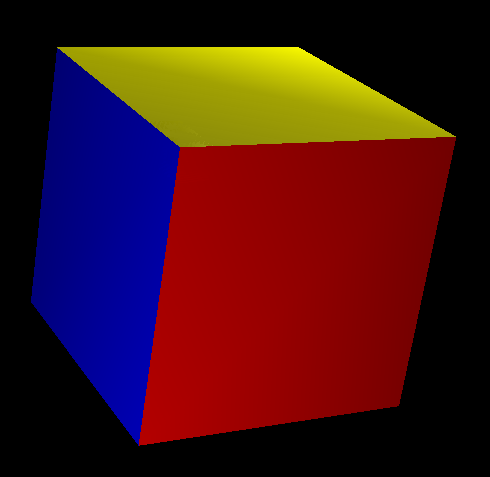
\includegraphics[width=6cm]{bildoj/menger0.png}
    \begin{center}
      \textbf{Stadio 0}
    \end{center}
  \end{minipage}
  \begin{minipage}{6cm}
    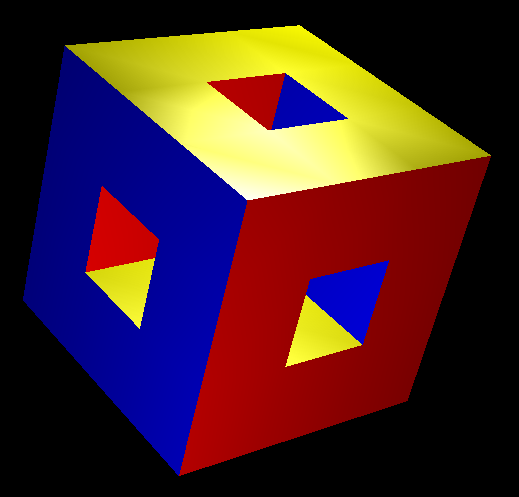
\includegraphics[width=6cm]{bildoj/menger1.png}
    \begin{center}
      \textbf{Stadio 1}
    \end{center}
  \end{minipage}
  \\
  \begin{minipage}{6cm}
    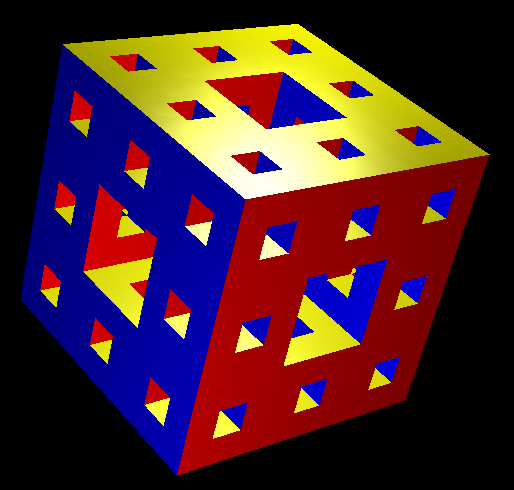
\includegraphics[width=6cm]{bildoj/menger2.png}
    \begin{center}
      \textbf{Stadio 2}
    \end{center}
  \end{minipage}
  \begin{minipage}{6cm}
    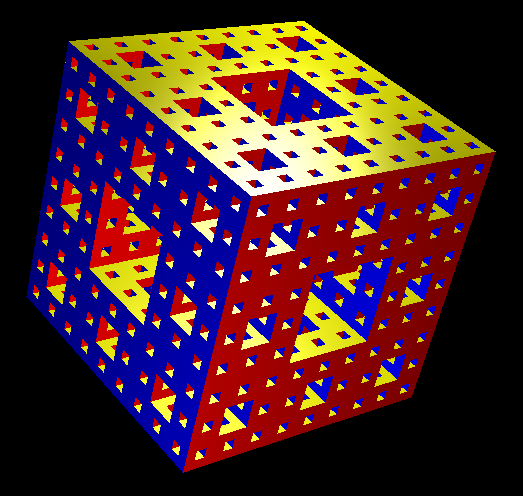
\includegraphics[width=6cm]{bildoj/menger3.png}
    \begin{center}
      \textbf{Stadio 3}
    \end{center}
  \end{minipage}
\end{center}

La ^capitro konsistas el du partoj:
\begin{itemize}
\item Anta^u ^cio, ni montros kiel krei tiun solidon facile per uzo
  de rekursiveco.
\item Poste, oni provos plibonigi la grafikadon por grafiki spongon de
  Menger de ordo~4.
\end{itemize}

\section{Uzante rekursivecon}

Konsideru spongon de Menger de ordo $n$ kies latero mezuras $L$.\\
\begin{center}
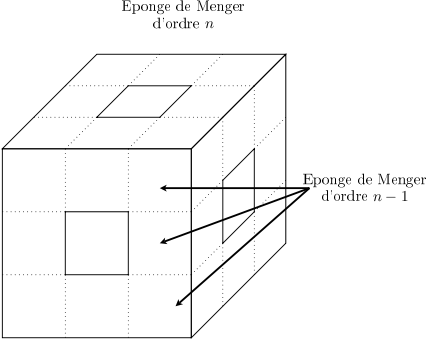
\includegraphics{bildoj/menger-schema01.png}
\end{center}
La skemo montras bone ke tiu spongo konsistas efektive el $20$ spongoj
de Menger de ordo $n-1$ havantaj ^ciuj lateron je ${L}/{3}$.  La
rekursiva strukturo de la spongo evidenti^gas tiel.

\textbf{La programo:}

\begin{verbatim}
# Ĉefa komando: spongo 3
por kubo :l
se :nombrilo = 10000 [tridimensie_vidigu]
# Koloroj de la flankaj facoj
lokp "koloroj [flavan violruĝan verdbluan bluan]
# flankaj facoj
ripetu 4 [skolp ekzek eron kmpt :koloroj kvadrato :l dn 90 an  :l mdn 90 dkn 90]
# Sube
skolp ruĝan malsupren 90 kvadrato :l supren 90
av :l msn 90 skolp verdan kvadrato :l sn 90 man :l
fino

por kvadrato :c
provizu "nombrilo :nombrilo + 1
por_edro
ripetu 4 [an :c dn 90]
fino_edro
fino

# Spongo de Menger
# p: profundeco de rekursiveco
# l: longeco de la granda kubo
por menger :l :p
se :p=0 [kubo :l] 
 [lokp "p :p-1  
  lokp "l :l/3
  # antaŭa faco
  ripetu 3 [menger :l :p an :l] man 3*:l
  dn 90 an :l mdn 90
  menger :l :p an 2*:l menger :l :p man 2*:l
  dn 90 an :l mdn 90
  ripetu 3 [menger :l :p av :l] man 3*:l
  # dekstra flanko
  malsupren 90 an :l supren 90 
  menger :l :p an 2*:l menger :l :p re 2*:l
  malsupren 90 an :l supren 90 
  ripetu 3 [menger :l :p an :l] man 3*:l
  mdn 90 an :l dn 90
  menger :l :p an 2*:l menger :l :p man 2*:l
  mdn 90 an :l dn 90
  ripetu 3 [menger :l :p an :l] man 3*:l
  malsupren 90 man :l supren 90
  menger :l :p an 2*:l menger :l :p man 2*:l
  malsupren 90 man :l supren 90]
fino

por spongo :p
ev tdk provizu "nombrilo 0 perspektive fkolp 0 menger 800 :p 
tajpu [Nombro de kvadratoj: ] s :nombrilo
tridimensie_vidigu
fino
\end{verbatim}

Tiu programo konsistas el kvar proceduroj:
\begin{itemize}
\item \texttt{kvadrato :c}\\
  Tiu proceduro grafikas kvadraton kun lateroj longaj je \texttt{:c}.
  Krome, tiun kvadraton registras la modelilo 3D.  La variablo
  \texttt{nombrilo} responsas pri nombri la nombron de kvadratojn
  desegnitajn.
\item \texttt{kubo :l}\\
  Tiu proceduro grafikas kubon kun lateroj longaj je \texttt{:l}.
  Kompreneble, ^gi uzas la proceduron \texttt{kvadrato}.
\item \texttt{menger :l :p}\\
  Tiu proceduro estas la ^cefa^jo de l' programo; ^gi desegnas motivon
  de Menger de ordo $p$ kaj do la latero mezuras $l$.  Tiun motivon
  oni kreas la^u rekursiva maniero tute nature sekvante la anta^uan
  skemon.
\item \texttt{spongo :p}\\
  Tiu proceduro grafikas spongon de Menger de ordo $p$ kaj kun latero
  $800$ kaj aldonas ^gin al modelilo 3D.
\end{itemize}
\vfill
\pagebreak

\section{Dua pritrakto: solida objekto de $4$-a ordo}

La anta^ua programo havas kiel ^cefan avanta^gon ekspluati la nature
rekursivan strukturon de la fraktala solido.  Rimarku ke tiu sama
metodo povas esti uzata anka^u por generi aliajn fraktalajn solidojn
a^u, pli simple, aliajn fraktalajn kurbojn.  ^Ciuokaze, la tuja
konsekvenco de la rekursiva pritrakto estas mallonga fontokodo kaj
simple komprenebla.  Beda^urinde, rimarku ke spongo je $3$-a ordo
postulas jam $48\,000$ kvadratojn.  Necesas tiam estigi la memoron
dediĉitan al XLogo je $256$ MB en la fenestro pri preferoj por ke la
programo povu ruli^gi tute.

Se oni deziras grafiki Menger-an spongon je $4$-a ordo, balda^u oni
estos barita de for^cerpado de memoro.  En ^ci tiu parto ni vidos
programon bazitan sur tute malsama algoritmo; ^gi ebligos krei spongon
de Menger je ordo $0$, $1$, $2$, $3$ a^u $4$.

\subsection{La tapi^so de Sierpinski}

La spongo de Menger estas efektive ^generaligon en $3$ dimensioj de
ebena figuno nomata \emph{tapi^so de Sierpinski}.  Jen la unuaj
iteracioj de tiu figuro:

\vspace{5mm}
\begin{minipage}{4.1cm}
\begin{center}
 
\includegraphics[width=4.0cm]{bildoj/carpet0.png}\\
\textbf{Stadio 0}
\end{center}
\end{minipage}
\begin{minipage}{4.1cm}
\begin{center}
 
\includegraphics[width=4.0cm]{bildoj/carpet1.png}\\
\textbf{Stadio 1}
\end{center}
\end{minipage}
\begin{minipage}{4.1cm}
\begin{center}
 
\includegraphics[width=4.0cm]{bildoj/carpet2.png}\\
\textbf{Stadio 2}
\end{center}
\end{minipage}
\begin{minipage}{4.1cm}
\begin{center}
 
\includegraphics[width=4.0cm]{bildoj/carpet3.png}\\
\textbf{Stadio 3}
\end{center}
\end{minipage}
\vspace{5mm}

La motivo estanta sur ^ciu faco de spongo de Menger je ordo $p$-a
estas tapi^so de Sierpinski je ordo $p$-a.

\subsection{Grafiki tapi^son de Sierpinski je ordo $p$-a}

La celo estas atingi malpligrandigi la nombron de postulitaj kvarlateroj
por desegni tapi^son de Sierpinski.  La jena ekzemplo klarigas la la
procedon uzitan por krei tapi^son de Sierpinski je ordo $3$-a.  ^Ci
tie, la komenca kvadrato konsistas do el $3^3=27$ horizontaloj kaj
$27$ vertikaloj.  Oni skribas je bazo $3$ la numeron de ^ciu
horizontalo kaj ^ciu vertikalo.

\begin{itemize}
\item [\textbullet]\textbf{Unua stadio:} Por ^ciu horizontalo kies
  numero konsistas el neniu $1$, grafiku horizontalon de $27$ ^celoj.
  Pro simetrio, efektivigu la saman operacion vertikale.
\begin{center}
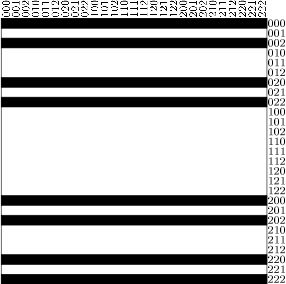
\includegraphics{bildoj/menger-schema02.png}
\includegraphics{bildoj/menger-schema03.png}
\end{center}
\vspace{0.2cm}
\item [\textbullet] \textbf{Dua stadio:} Nun interesi^gu pri la
  horizontaloj kies numero konsistas el ununura $1$ en l' unua loko.
  Grafiku sinsekve alterne ortangulojn longaj je $9$ ^celoj.  Faru
  por la vertikaloj simetrie.
\begin{center}
\includegraphics{bildoj/menger-schema04.png}
\end{center} 
\item [\textbullet] \textbf{Tria stadio:} Nun interesi^gu pri la
  horizontaloj kies numero konsistas el nur unu $1$ en la dua loko.
  Grafiku sinsekve alterne ortangulojn la^u la skemo $[3\ 3\ 6\ 3\ 6\
  3\ 3]$ ($3$ ^celoj plenaj, $3$ malplenaj, $6$ plenaj, ktp...).
  Simetrie faru por la vertikaloj.
\begin{center}
\includegraphics{bildoj/menger-schema05.png}
\end{center}
\item [\textbullet] \textbf{Lasta stadio:} Interesi^gu pri
  horizontaloj kies numero konsistas el du $1$ lokitaj en l' unuaj
  lokoj.  Grafiku sinsekve alterne ortangulojn la^u la skemo $[3\ 3\
  3\ 9\ 3\ 3\ 3]$.  Operaciu same por la vertikaloj.
\begin{center}
\includegraphics{bildoj/menger-schema06.png}
\end{center}
\end{itemize}
Tiam fini^gas la konstruado de la tapi^so de Sierpinski je ordo $3$-a.
Por krei tiun tapi^son necesis uzi entute: $16+16+32+16=80$
ortangulojn.

\subsection{Malsamaj skemoj de vertikaloj eblaj}

Por resumi la anta^uan konstruadon, jen la malsamaj tipoj de skemaj de
vertikaloj la^u ilia numero.  (La simbolo * indikas la ciferon $0$ a^u
la ciferon $2$.
\begin{center}
  \begin{tabular}{|c|c|}
    \hline
    Numero de la tipo & Skemo aplikenda \\
    \hline
    *** & 27 \\ 
    \hline
    1** &  9 9 9 \\
    \hline
    *1* & 3 3 6 3 6 3 3\\
    \hline
    11* & 3 3 3 9 3 3 3\\
    \hline
  \end{tabular}
\end{center}

Sur la sama principo, por krei tapi^son je ordo $4$-a, oni uzu
kvadraton kun $3^4=81$ ^celoj.  La numeroj de horizontaloj kaj
vertikaloj havos do $4$ ciferojn en ilia prezentado je bazo $3$.  Por
^ciu tipo de numero, jen la skemo aplikenda (la simbolo * indikas la
ciferon $0$ a^u la ciferon $2$):

\begin{center}
 \begin{tabular}{|c|c|}
 \hline
Numero de tipo & Skemo aplikenda \\
\hline
 **** & 81 \\ 
\hline
1*** &  27 27 27 \\
\hline
*1** & 9 9 18 9 18 9 9 \\
\hline
**1* & 3 3 6 3 6 3 6 3 6 3 6 3 6 3 6 3 6 3 3 \\
\hline
*11* &  3 3 3 9 3 3 6 3 3 9 3 3 6 3 3 9 3 3 3 \\
\hline
1*1* & 3 3 6 3 6 3 3 27 3 3 6 3 6 3 3 \\
\hline
11** & 9 9 9 27 9 9 9 \\
\hline
111*& 3 3 3 9 3 3 3 27 3 3 3 9 3 3 3 \\
\hline
\end{tabular}\\
$496$ kvarlateroj estas do necesaj por grafiki tapi^son de Sierpinski je ordo $4$.
\end{center}

Finfine, jen la konstruskemoj por solidoj je ordo $2$:
\begin{center}
  \begin{tabular}{|c|c|}
 \hline
Numero de tipo & Skem' aplikenda \\
\hline
** &  9 \\
\hline
1* & 3 3 3 \\ 
\hline
\end{tabular}
\end{center}

\subsection{La programo}
\begin{verbatim}
# Grafikas tapi^son de Sierpinski je ordo :p kaj je amplekso :amplekso
por tapiŝo :amplekso :p
provizu "unuo :amplekso / (potencon 3 :p)
se :p=0 [ort :amplekso :amplekso haltu]
se :p=1 [ripetu 4 [ort :amplekso :unuo an :amplekso dn 90] haltu]
ripetupor (list "x 1 potencon 3 :p) 
  [lokp "cantorx cantor :x :p []
  # Ne grafiku la erojn havantajn unu 1 en la lasta loko
  se  ne (1 = lastan :cantorx)
    [lokp "nom valorigu senlastan :cantorx "
     grafiku_vertikalon :x econ_sendu "map :nom]]  
fino

# Donas la nombron x je bazo 3
# p profundeca indekso 3^p
# :list listo malplena ĉe l' komenco

por cantor :x :p :list
se :p=0 [sendu :list] 
lokp "a potencon 3 :p-1
se :x <= :a 
  [sendu cantor :x :p-1 frazon :list 0] 
  [se :x <= 2*:a [sendu cantor  :x-:a :p-1 frazon :list 1] 
   sendu cantor :x - 2*:a :p-1 frazon :list 0]
fino

# Grafiku la x-an vertikalon laŭ la konstruskemo difinita en la listo
por grafiku_vertikalon :x :list
  l  dn 90 an (:x-1)*:unuo mdn 90 ml des :list
  l mdn 90 an (:x-1)*:unuo mdn 90 an :x*:unuo dn 90 ml des :list
l mdn 90 man :x*:unuo ml
fino

# Grafiku ortangulon laŭ donitaj dimensioj
# Ĝin registras la 3d-vidilo
por ort :lo :la
provizu "nombrilo :nombrilo + 1
por_edro
ripetu 2 [an :lo dn 90 an :la dn 90]
fino_edro
fino

# Pretigu la malsamajn eblajn vertikalojn por la tapiŝoj je ordo 1 al 4
por pretmap
econ_provizu "map 111 [3 3 3 9 3 3 3 27 3 3 3 9 3 3 3]
econ_provizu "map 110 [9 9 9 27 9 9 9]
econ_provizu "map 101 [3 3 6 3 6 3 3 27 3 3 6 3 6 3 3]
econ_provizu "map 011 [3 3 3 9 3 3 6 3 3 9 3 3 6 3 3 9 3 3 3]
econ_provizu "map 000 [81]
econ_provizu "map 100 [27 27 27]
econ_provizu "map 010 [9 9 18 9 18 9 9]
econ_provizu "map 001 [3 3 6 3 6 3 6 3 6 3 6 3 6 3 6 3 6 3 3]
econ_provizu "map  01 [3 3 6 3 6 3 3]
econ_provizu "map  00 [27]
econ_provizu "map  10 [9 9 9]
econ_provizu "map  11 [3 3 3 9 3 3 3]
econ_provizu "map   1 [3 3 3]
econ_provizu "map   0 [9]
fino

# Se la prezento estas [1 0 1] --> sendu 101
por valorigu :list :vort
  se malplena? :list [sendu :vort]
  [lokp "vort vort :vort unuan :list
   sendu valorigu senunuan :list :vort]
fino

# Desegnu la ortangulojn de ĉiu vertikalo alterne
por des :list
lokp "sumo 0
ripetupor (list "i 1 kmpt :list) 
   [lokp "ero eron :i :list
    lokp "sumo :ero + :sumo
    se para? :i [l an :ero*:unuo ml] [ort :ero*:unuo :unuo an :ero*:unuo]]
l man :sumo * :unuo ml
fino

# Testu ĉu nombro estas para
por para? :i
sendu 0 = reston :i 2
fino

por siertapiŝo :p
ev perspektive tdk pretmap
provizu "nombrilo 0
tapiŝo 810 :p
tajpu "Nombro\ de\ kvarlateroj:\  s :nombrilo
vue3d
fin
\end{verbatim}

\texttt{siertapi^so 3} desegnas tapi^son de Sierpinski je ordo $3$ kaj
latero $810$.  Jen, ni pretas pasi al la spongo de Menger!

\subsection{La spongo de Menger je ordo 4}

La spongo de Menger havas plurajn simetriecajn atributojn.  Por generi
^gin ni grafikos la diversajn sekciojn la^u la ebeno $(xOy)$, poste
portos tiujn figurojn la^u $(yOz)$ kaj $(xOz)$. Por bone klarigi tion
kio okazas, ni restu sur l' ekzemplo de la spongo je ordo $3$:

Kiam oni tran^cas la spongon la^u vertikala ebeno, oni povas akiri kvar malsamajn motivojn:
\vspace*{0.6cm}
 \begin{center}
\includegraphics{bildoj/menger-schema07.png}\\ \vspace{0.5cm}
\includegraphics{bildoj/menger-schema08.png}\\ \vspace{0.5cm}
\includegraphics{bildoj/menger-schema09.png}\\ \vspace{0.5cm}
\includegraphics{bildoj/menger-schema10.png}\\ 
\end{center}

Por grafiki spongon je ordo $3$, ni trairos la nombrojn de $1$ ^gis
$27$, tio estas, de $001$ ^gis $222$ je bazo $3$.  Por ^ciu numero,
oni aplikos la ta^ugan sekcion kiun oni portos la^u la $3$ direktoj
$(Ox)$, $(Oy)$ kaj $(Oz)$.

\subsubsection{La kodo}

La jena programo permesas grafiki la solidojn de Menger je ordoj $0$,
$1$, $2$, $3$, $4$.  La nombro de proceduroj estas grava, do mi
klarigos tuj.

\begin{verbatim}
# Grafiki tapiŝon de Sierpinski je ordo :p kaj je amplekso :amplekso
por  tapiŝo :amplekso :p
provizu "unuo :amplekso / (potencon 3 :p)
se :p=0 [ort :amplekso :amplekso haltu]
se :p=1 [ripetu 4 [ort :amplekso :unuo an :amplekso dn 90] haltu]
ripetupor (list "x 1 potencon 3 :p) 
  [lokp "cantorx cantor :x :p []
   # Ne grafiku erojn havantajn unu 1 en la lasta loko
   se  ne (1 = lastan :cantorx)  
     [lokp "nom valorigu senlastan :cantorx "
      grafikuvertikalon :x econ_sendu "map :nom]]  
fino

# Sendu la prezenton je bazo 3 de la nombro x
# p profundeca indekso 3^p
# :list listo malplena ĉe l' komenco

por cantor :x :p :list
se :p=0 [sendu :list] 
lokp "a potencon 3 :p-1
se :x <= :a 
  [sendu cantor :x :p-1 frazon :list 0] 
  [se :x <= 2*:a [sendu cantor :x-:a :p-1 frazon :list 1]
   sendu cantor :x-2*:a :p-1 frazon :list 2]
fino

# Grafiku la numeron x laŭ la konstruskemo difinita en la listo
por grafikuvertikalon :x :list
  l  dn 90  an (:x-1)*:unuo mdn 90 ml des :list
  l mdn 90  an (:x-1)*:unuo  dn 90 an :x*:unuo dn 90 ml des :list
  l mdn 90 man :x*:unuo ml
fino

# Grafiku ortangulon laŭ donitaj dimensiojn
# La plurlatero estas registrita de la 3d-vidigilo
por ort :lo :la
  provizu "nombrilo :nombrilo+1
  por_edro
    ripetu 2 [an :lo dn 90 an :la dn 90]
  fino_edro
fino

# Komencu la malsamajn vertikalojn eblajn por la tapiŝojn je ordo 1 ĝis 4
por pretmap
econ_sendu "map 111 [3 3 3 9 3 3 3 27 3 3 3 9 3 3 3]
econ_sendu "map 110 [9 9 9 27 9 9 9]
econ_sendu "map 101 [3 3 6 3 6 3 3 27 3 3 6 3 6 3 3]
econ_sendu "map 011 [3 3 3 9 3 3 6 3 3 9 3 3 6 3 3 9 3 3 3]
econ_sendu "map 000 [81]
econ_sendu "map 100 [27 27 27]
econ_sendu "map 010 [9 9 18 9 18 9 9]
econ_sendu "map 001 [3 3 6 3 6 3 6 3 6 3 6 3 6 3 6 3 6 3 3]
econ_sendu "map  01 [3 3 6 3 6 3 3]
econ_sendu "map  00 [27]
econ_sendu "map  10 [9 9 9]
econ_sendu "map  11 [3 3 3 9 3 3 3]
econ_sendu "map   1 [3 3 3]
econ_sendu "map   0 [9]
fino

# Se la prezento estas [1 0 1] --> sendu 101
# Se la prezento estas [1 0 2] --> sendu 100
# La eroj de la listo estas kunmetataj en vorton.
# Krome, la 2 estas anstataŭataj de nuloj
por valorigu :list :vort
  se malplena? :list [sendu :vort]
    [lokp "unua unuan :list
     se :unua=2 [lokp "unua 0] 
     lokp "vort vort :vort :unua
     sendu valorigu senunuan :list :vort]
fino

# Desegnu la ortangulojn de ĉiu vertikalo alterne
por des :list
lokp "sumo 0
ripetupor (liston "i 1 kmpt :list) 
   [lokp "ero eron :i :list
    lokp "sumo :ero+:sumo 
    se para? :i [l an :ero*:unuo ml] [ort :ort*:unuo :unuo an :ero*:unuo]]
l man :sumo * :unuo ml
fino

# Testu ĉu nombro estas para
por para? :i
  sendu 0 = resto :i 2
fino

por siertapiŝo :p
  ev perspektive tdk pretmap
  provizu "nombrilo 0
  tapiŝo 810 :p
  tajpu "Nombro\ de\ plurlateroj:\  s :nombrilo 
  tridimensie_vidigu
fino

# Forigas la lastan 1 en la listo :list
por forigulastanunu :list
  ripetupor (list "i kmpt :list 1 minusigan 1) 
    [lokp "ero eron :i :list 
     se :ero=1 [lokp "list anstataŭigu :list :i 0 haltu] [se :ero=2 [haltu]]]
  sendu :list
fino

# Spongo de Menger je amplekso donita kaj je profundeco :p

por menger :amplekso :p
provizu "unuo :amplekso / (potencon 3 :p)
ripetupor (list "z 1 potencon 3 :p) 
  [lokp "cantorz cantor :z :p []
   lokp "last lastan :cantorz
   lokp "cantorz senlantan :cantorz
   se :last=0 [lokp "ordo valorigu forigulastanunu :cantorz "] [lokp "ordo valorigu :cantorz "]
   lokp "ordo vort "tranĉi :ordo
   graf3tapiŝon :amplekso :ordo :z
   l supren 90 an :unuo malsupren 90 ml]
graf3tapiŝon :amplekso :ordo (potencon 3 :p) + 1
fino

# Grafiku la tapiŝojn de Sierpinski je ordo :p
# laŭ ĉiu akso (Ox), (Oy) et (Oz)
# je la alto :z
pour draw3carpet :size :order :z
  l originen
  supren 90 an (:z-1)*:unuo malsupren 90 ml
  skolp bluan ekzek :ordo :amplekso
  l originen
  mdfn 90 an (:z-1)*:unuo malsupren 90 ml
  skolp flavan ekzek :ordo :amplekso
  l originen  
  supren 90 an :amplekso dn 90 an (:z-1)*:unuo malsupren 90 ml
  skolp violruĝan ekzek :ordo :amplekso
fino

# Ĉefa proceduro
# Grafiku spongon de Menger je profundeco :p
por spongo :p
  ev perspektive tdk
  lokp "tempo tempon
  pretmap
  provizu "nombrilo 0
  se :p=0 [kubo 405] [menger 405 :p]
  # Skribu la tempon kaj la nombron de plurlateroj necesaj por konstrui
  tajpu "Nombro\ de\ plurlateroj:\  s :nombrilo
  tajpu "Tempo\ uzita:\  s tempon - :tempo
  tridimensie_vidigu
fino

# Sekcio por la Menger je ordo 2

por tranĉi1 :amplekso
  ripetu 4 [tapiŝu :amplekso/3 1 l an :amplekso dn 90 ml]
fino

por tranĉi0 :amplekso
  tapiŝo :amplekso 2
fino

# Sekcio por la Menger je ordo 3

por tranĉi10 :amplekso
  ripetu 4 [tapiŝo :amplekso/3 2 l an :amplekso dn 90 ml]
fino

por tranĉi01 :amplekso
  ripetu 4 [ripetu 2 [tranĉi1 :amplekso/3 l an :amplekso/3 ml] an :amplekso/3 dn 90]
fino

por tranĉi11 :amplekso
  ripetu 4 [tranĉi1 :amplekso/3 l an :amplekso dn 90 ml]
fino

por tranĉi00 :amplekso
  tapiŝo :amplekso 3
fino

# Sekcio por la Menger je ordo 4

por tranĉi000 :amplekso
  tapiŝo :amplekso 4
fino

por tranĉi100 :amplekso
  ripetu 4 [tapiŝo :amplekso/3 3 l an :amplekso dn 90 ml]
fino

por tranĉi010 :amplekso
  ripetu 4 [ripetu 2 [tranĉi10 :amplekso/3 l an :amplekso/3 ml] an :amplekso/3 dn 90]
fino

por tranĉi001 :amplekso
  ripetu 4 [ripetu 2 [tranĉi01 :amplekso/3 l an :amplekso/3 ml] an :amplekso/3 dn 90]
fino

por tranĉi110 :amplekso
  ripetu 4 [tranĉi10 :amplekso/3 l an :amplekso ml dn 90]
fino

por tranĉi111 :amplekso
  ripetu 4 [tranĉi11 :amplekso/3 l an :amplekso dn 90 ml]
fino

por tranĉi101 :amplekso
  ripetu 4 [tranĉi01 :amplekso/3 l an :amplekso dn 90 ml]
fino

por tranĉi011 :amplekso
  ripetu 4 [ripetu 2 [tranĉi11 :amplekso/3 l an :amplekso/3 ml] an :amplekso/3 dn 90]
fino

por tranĉi :amplekso
  tapiŝo :amplekso 1
fino

por kubo :amplekso
  ripetu 2 
    [skolp bluan  ort :amplekso :amplekso l an :amplekso malsupren 90 ml
     skolp flavan ort :amplekso :amplekso l an :amplekso malsupren 90 ml]
  skolp violruĝan
  l mdfn 90 mdn 90 an :amplekso dn 90 ml ort :amplekso :amplekso
  l dn 90 an :amplekso mdn 90 dfn 90 dn 90 an :amplekso mdn 90 dfn 90 ml ort :amplekso :amplekso
  mdfn 90 mdn 90 an :amplekso dn 90
fino

por kuboj
  ev perspektive tdk
  lokp "tempo tempon
  pretmap
  provizu "nombrilo 0
  ripetu 4 [se komputu = 1 [kubo 405] [menger 405 komputu-1] l an 1000 dn 90 ml]
  # Montru la tempon uzitan kaj la nombron de plurlateroj necesaj por konstrui
  tajpu "Nombro\ de\ plurlateroj:\  s :nombrilo
  tajpu "Tempo\ uzita:\  s tempon - :tempo
  tridimensie_vidigu
fino
\end{verbatim}

Nun, establu la memoron rezervitan por \xlogo\ je 640 MiB: \texttt{spongo 4}
\begin{center}
 \includegraphics{bildoj/menger-menger4.png}
\end{center}

\chapter{Temo: Sistemo de Lindenmayer}

{ }\hfill\textbf{Nivelo:} Alta

Por ^ci tiu parto, mi indiku kelkajn refera^jojn:
\begin{itemize}
 \item de la retpa^go Vikipedio pri la L-sistemoj: \texttt{http://eo.wikipedia.org/wiki/L-Sistemo}.
 \item de la libro \og The Algorithmic Beauty of Plants\fg{} verkita
   de Przemyslaw Prusinkiewicz kaj Aristid Lindenmayer.
\end{itemize}

\vspace*{0.5cm} 

Temos pri la nocio de sistemo de Lindenmayer a^u L-sistemo inventita
en 1968 de la biologo hungaro Aristid Lindenmayer.  L-Sistemo estas
aro da reguloj kaj simboloj kiuj modelas procezon de kreskado de
vivuloj kiel plantoj a^u ^celoj.  La ^cefa koncepto de la L-sistemoj
estas la nocio de reskribado.  Reskribado estas te^hniko por konstrui
malsimplajn objektojn per anstata^uigi partojn de komenca simpla
objekto uzante regulojn de reskribado.

Por fari tion, la ^celoj estas modelitaj per simboloj.  Je ^ciu
generacio, la ^celoj disparti^gas, tio estas, simbolon anstata^uas unu
a^u pluraj aliaj simboloj formantaj vorton.

\section{Formala difino}

L-sistemo estas formala gramatiko konsistanta el:
\begin{enumerate}
\item Unu alfabeto $V$: l' aro de la variabloj de la L-Sistemo. $V *$
  estas la aro de la ``vortoj'' kiujn oni povas konstrui per la simboloj
  de $V$, kaj $V +$ l' aro de la vortoj enhavantaj almena^u unu simbolon.
\item Unu aro de valoroj konstantaj $S$.  Kelkaj el tiuj simboloj
  estas komunaj al ^ciuj L-Sistemoj (^cefe kiam uzi la testudon).
\item Unu komenca aksiomo $\omega$ elektita inter $V +$ , tio estas la
  komenca stato.
\item Unu ekzemplo de reguloj, indikata $P$, pri reproduktado de la
  simboloj de $V$.
\end{enumerate}

L-sistemo estas do indikata $\{V,S,\omega,P\}$.

Konsideru la jenan L-sistemon:
\begin{itemize}
\item Alfabeto: $V = \{A, B\}$
\item Konstantoj: $S = \{\emptyset\}$
\item Komenca aksiomo: $\omega = A$
\item Reguloj: 
  $\begin{array}{|l|}
    \hline
    A \rightarrow AB \\
    B \rightarrow A \\ 
    \hline
  \end{array}$
\end{itemize}
La du reguloj donitaj estas la reguloj de reskribado de la sistemo.
Je ^ciu stadio, $A$ estas anstata^uita de la sinsekvo $AB$, kaj $B$
estas anstata^uita de $A$.  Jen la unuaj iteracioj de tiu sistemo de
Lindemayer:
\begin{center}
  \includegraphics[width=8cm]{bildoj/linden-arbre.png}
\end{center}
\begin{itemize}
\item Iteracio 1: $A$
\item Iteracio 2: $AB$
\item Iteracio 3: $ABA$
\item Iteracio 4: $ABAAB$
\end{itemize}
\vspace*{0.2cm}
Bone, bone... sed konkrete? Da^urigu legi!

\section{Interpretado de la testudo}

Tiu unua ekzemplo ebligis vin kompreni la nocion de sistemo de
Lindenmayer, eble sen ekkonscii kiel ni uzos tion konkrete kun la
testudo.

Ja tie tio esti^gas interesa: ^Ciu vorto tiel konstruita nur havas
propran signifon.  Oni tiam kro^cos al ^ciu litero de la sinsekvo,
komandon rulotan de la testudo, por tiel generi desegnojn 2D a^u 3D.

\subsection{Oftaj simboloj}
\begin{itemize}
 \item [\textbullet] $F$ : Movi^gi je unu unueca pa^so ($\in V$)
 \item [\textbullet] $+$ : Turni^gi maldekstren je angulo $\alpha$ $(\in S)$.
 \item [\textbullet] $-$ : Turni^gi dekstren je angulo $\alpha$ $(\in S)$.
 \item [\textbullet] $\&$ : Pivoti al malsupro je angulo $\alpha$ $(\in S)$.
 \item [\textbullet] \textasciicircum : Pivoti al supro je angulo $\alpha$ $(\in S)$.
 \item [\textbullet] \textbackslash: Ruli^gi maldekstren je angulo $\alpha$ $(\in S)$.
 \item [\textbullet] $/$: Ruli^gi dekstren je angulo $\alpha$ $(\in S)$.
 \item [\textbullet] $|$: Efektivigi duonturni^gon.  En XLogo: \texttt{dn 180}
\end{itemize}
\vspace*{0.2cm}
Ni prenu por ekzemplo $\alpha=90$ kaj unuecan movi^gon je $10$ testudpa^sojn; jen:
\begin{center}
 \begin{tabular}{|c|c|c|c|c|c|c|c|c|}
 \hline
Simbolo & $F$ & $+$ & $-$ & $\&$ & \textasciicircum & \textbackslash& $/$ & $|$ \\
 \hline
Komando XLogo & \texttt{an 10}&\texttt{mdn 90}&\texttt{dn 90}&\texttt{malsupren 90}&\texttt{supren 90}&\texttt{mdfn 90}&\texttt{dfn 90}&\texttt{dn 180}\\
 \hline
\end{tabular}
\end{center}
\subsection{Ne^gero de Koch}
Konsideru la L-sistemon:
\begin{itemize}
 \item [\textbullet] Komenca stato: $F--F--F--$
 \item [\textbullet] Produkta regulo: $F \rightarrow F+F--F+F$
 \item [\textbullet] Angulo $\alpha=60$\degre, la unuecan pa^son oni dividu per $3$ 
   je ^ciu iteracio.
\end{itemize}
Unuaj iteracioj:
\begin{center}
\begin{minipage}{7.5cm}
 \includegraphics[width=7.5cm]{bildoj/linden-flocon1.png}
\end{minipage}
\begin{minipage}{7.5cm}
 \includegraphics[width=7.5cm]{bildoj/linden-flocon2.png}
\end{minipage}\\
\begin{minipage}{7.5cm}
 \includegraphics[width=7.5cm]{bildoj/linden-flocon3.png}
\end{minipage}
\begin{minipage}{7.5cm}
 \includegraphics[width=7.5cm]{bildoj/linden-flocon4.png}
\end{minipage}
\end{center}
Programo en Logo:
\begin{verbatim}
por neĝero :p
provizu "unuo 300 / potencon 3 :p-1
ripetu 3 [F :p-1 td 120]  
fino

por F :p
se :p=0 [an :unuo haltu]
F :p-1 mdn 60 F :p-1 dn 120 F :p-1 md 60
F :p-1 
fino
\end{verbatim}

\subsection{Kurbo de Koch je ordo 2}
Ni interesi^gu pri la jena L-sistemo:
\begin{itemize}
 \item[\textbullet] Komenca stato: $F-F-F-F$
 \item[\textbullet] Produkta regulo: $F\rightarrow F-F+F+FF-F-F+F$
\end{itemize}

Jen la unuaj reprezentoj uzante $\alpha=90$ kaj alĝustigante la unuecan pa^son tiel ke
la figuro havu ^ciam la saman amplekson:
\begin{center}
\begin{minipage}{7.5cm}
 \includegraphics[width=7.5cm]{bildoj/linden-koch1.png}
\end{minipage}
\begin{minipage}{7.5cm}
 \includegraphics[width=7.5cm]{bildoj/linden-koch2.png}
\end{minipage}\\
\begin{minipage}{7.5cm}
 \includegraphics[width=7.5cm]{bildoj/linden-koch3.png}
\end{minipage}
\begin{minipage}{7.5cm}
 \includegraphics[width=7.5cm]{bildoj/linden-koch4.png}
\end{minipage}
\end{center}
Tre facilas do krei la programon Logo ebligantan generi tiujn desegnojn:
\begin{verbatim}
# p indikas l' iteracion
por koch :p
  # Je ĉiu iteracio, la unueca distanco dividatas per 4
  # Ĉi tie, la fina figuro havos amplekson 600x600 maksimume
  provizu "unuo 300 / potencon 4 :p-1
  ripetu 3 [F :p-1 tg 90] F :p-1 
fino

# La ĉeno reskribada
por F :p
  se :p=0 [an :unuo haltu]
  F :p-1 mdn 90 F :p-1 dn 90 F :p-1 dn 90
  F :p-1 F :p-1 mdn 90 F :p-1 mdn 90 F :p-1 dn 90 F :p-1
fino
\end{verbatim}

\subsection{Kurbo de l' dragono}
\begin{itemize}
 \item[\textbullet] Komenca stato: $F$\\
 \item[\textbullet] Produkta regulo: $\begin{array}{|l|}
\hline
A\rightarrow A+B+ \\
B\rightarrow -A-B \\
\hline
\end{array}$ 
\end{itemize}
\begin{verbatim}
por a :p
se :p=0 [an :unuo haltu]
a :p-1 mdn 90 b :p-1 mdn 90
fino

por b :p
se :p=0 [an :unuo haltu]
dn 90 a :p-1 dn 90 b :p-1
fino

por dragono :p
provizu "unuo 300 / 8 / :p  
a :p
fino
\end{verbatim}
\begin{center}
 \begin{minipage}{7cm}
 \includegraphics[width=7cm]{bildoj/linden-dragon10.png}
 \begin{center}
  \texttt{dragono 10}
 \end{center}
\end{minipage}
 \begin{minipage}{7cm}
 \includegraphics[width=7cm]{bildoj/linden-dragon15.png}
 \begin{center}
  \texttt{dragono 15}
 \end{center}
\end{minipage}
\end{center}

\subsection {Kurbo de Hilbert en 3D}

La sekva ekzemplo estas la kurbo de Hilbert en la spaco; ^gi estas
kurbo kun la atributo plenigi tute kubon kiam oni pligrandigas la
nombron de iteracioj .

Jen la rilata sistemo:
\begin{itemize}
 \item Komenca stato: $A$
 \item Angulo $\alpha=90$\degre, dividu la unuecan longon per du je
   ^ciu iteracio.
 \item Produkta regulo: 
   $\begin{array}{|l|}
     \hline
     A\rightarrow B-F+CFC+F-D\&F \textrm{\textrm{\textasciicircum}} D-F+\&\&CFC+F+B// \\
     B\rightarrow A\&F\textrm{\textrm{\textasciicircum}} CFB\textrm{\textasciicircum} F 
     \textrm{\textasciicircum} D\textrm{\textasciicircum} \textrm{\textasciicircum}-F-D
     \textrm{\textasciicircum}|F\textrm{\textasciicircum} B|FC\textrm{\textasciicircum} 
     F\textrm{\textasciicircum} A// \\
     C\rightarrow|D\textrm{\textasciicircum}|F\textrm{\textasciicircum} B-F+C\textrm{\textasciicircum} 
     F\textrm{\textasciicircum} A\&\&FA\&F\textrm{\textasciicircum} C+F+B\textrm{\textasciicircum} F
     \textrm{\textasciicircum} D// \\
     D\rightarrow|CFB-F+B|FA\&F\textrm{\textasciicircum} A\&\&FB-F+B|FC// \\
     \hline
   \end{array}$
\end{itemize}
\begin{verbatim}
por hilbert :p
ev perspektive
provizu "unuo 400 / potencon 2 :p
linia_difino sdikp :unuo/2
a :p
linia_difinhalto
tridimensie_vidigu
fino

por a :p
se :p=0 [haltu]
b :p-1 dn 90 an :unuo mdn 90 c :p-1 an :unuo c :p-1
mdn 90 an :unuo dn 90 d :p-1 malsupren 90 an :unuo supren 90 d :p-1
dn 90 an :unuo mdn 90 malsupren 180 c :p-1 an :unuo c :p-1
mdn 90 an :unuo mdn 90 b :p-1 dfn 180
fino

por b :p
se :p=0 [haltu]
a :p-1 malsupren 90 an :unuo supren 90 c :p-1 an :unuo b :p-1 supren 90 
an :unuo supren 90 d :p-1 supren 180 dn 90 an :unuo dn 90 d :p-1 supren 90 
dn 180 an :unuo supren 90 b :p-1 dn 180 an :unuo c :p-1 supren 90 an :unuo
supren 90 a :p-1 dfn 180 
fino

por c :p
se :p=0 [haltu]
dn 180 d :p-1 supren 90 dn 180 an :unuo supren 90 b :p-1 dn 90 an :unuo mdn 90 
c :p-1 supren 90 an :unuo supren 90 a :p-1 malsupren 180 an :unuo a :p-1 malsupren 90 
an :unuo supren 90 c :p-1 mdn 90 an :unuo mdn 90 b :p-1 supren 90 an :unuo supren 90 
d :p-1 dfn 180 
fino

por d :p
se :p=0 [haltu]
dn 180 c :p-1 an :unuo b :p-1 dn 90 an :unuo mdn 90 b :p-1 dn 180
an :unuo a :p-1 malsupren 90 an :unuo supren 90 a :p-1 malsupren 180 an :unuo
b :p-1 dn 90 an :unuo mdn 90 b :p-1 dn 180 an :unuo c :p-1 dfn 180
fino
\end{verbatim}
Jen l' unuaj iteracioj:
\begin{center}
\begin{minipage}{7cm}
 \includegraphics[width=7cm]{bildoj/linden-hilbert1.png}
\end{minipage}
\begin{minipage}{7cm}
 \includegraphics[width=7.5cm]{bildoj/linden-hilbert2.png}
\end{minipage}\\
\begin{minipage}{7cm}
 \includegraphics[width=7cm]{bildoj/linden-hilbert3.png}
\end{minipage}
\begin{minipage}{7cm}
 \includegraphics[width=9cm]{bildoj/linden-hilbert4.png}
\end{minipage}
\end{center}

\appendix
\chapter {Listo de la primitivoj}
\label{liste-prim} 

Kiel dirite anta^ue, oni kontrolas la testudon per internaj komandoj
nomataj prakomandoj a^u \og primitivoj\fg.  Jen klasado de tiuj
primitivoj:

\section{Movi la testudon, administri la krajonon kaj la kolorojn}
\subsection{Movi}
Primitivoj por movi la testudon.

\prim{anta^uen, an, antauen, antawen, antauxen} {n}
Movas la testudon anta^uen je $n$ pa^soj la^u la nuna direkto.

\prim{malanta^uen, man, malantauen, malantawen, malantauxen}{n}
Movas la testudon malanta^uen je $n$ pa^soj la^u la nuna direkto.

\prim{dekstren, dn}{n}
Turnas la testudon je $n$ gradoj dekstren rilate al la nuna direkto.

\prim{maldekstren, mdn}{n}
Turnas la testudon je $n$ gradoj maldekstren rilate al la nuna direkto.

\prim{rondon\_desegnu, rond}{R}
Desegnas cirklon kun radiuso R ^cirka^u la testudo.

\prim{arkon\_desegnu, ark}{R angulo1 angulo2}
Grafiki cirklan arkon kun radiuso R ^cirka^u la testudo, de la angulo 
1 ^gis la angulo 2.  (Angulo 0 estas alsupre kaj 
kreskas horlo^ge.)

\prim{originen, o}{}
Remetas la testudon en ^gian komencan situon, tio estas, en la punkton
kun koordinatoj {[}0 0{]} kaj rigardanta supren.

\prim{situon\_provizu, sitp}{listo}
Movas la testudon en punkton kun koordinatoj indikitaj de la listo de 
du nombroj (absciso kaj ordinato).

\prim{x\_provizu, xp}{x}
Movas horizontale la testudon ^gis la punkto kun absciso x.

\prim{y\_provizu, yp}{y}
Movas vertikale la testudon ^gis la punkto kun ordinato x.

\prim{xy\_provizu,xyp}{x y}
 Same kiel sitp{[}x y{]}

\prim{direkton\_provizu, dirp}{n}
Direktas la testudon al la angulo indikita.  $0$ signifas vertikale 
alsupre; turni kiel indikiloj de horlo^go.

\prim{etikedu, etik}{vortolisto}
Desegnas la vorton a^u la liston indikitan, tie kie trovi^gas 
la testudo kaj la^u ^gia inklino.
Ekzemple: \texttt{etikedu [Saluton al vi]} skribos la frazon 
\og Saluton al vi\fg{} tie kie estas lokita la testudo
kaj respektante la direkton de ^gi.

\prim{punkton\_montru, punkt}{listo}
^Saltas la punkton difinitan de la koordinatoj de la listo (je la 
koloro de krajon').

\subsection{Atributoj de la testudo}

La primitivoj prezentotaj ^ci tie ebligas modifi l' atributojn de la
testudo.  Por ekzemplo, ^cu necesas ke la testudo estu videbla sur l'
ekrano?  Je kiu koloro ^gi skribu kiam ^gi movi^gos?

\prim{testudon\_montru, tdm}{}
Videbligu la testudon sur l' ekrano.

\prim{testudon\_ka^su, tdk}{}
Malvidebligu la testudon sur l' ekrano.

\prim{ekranon\_vi^su, ev}{}
Forvi^su la desegnejon kaj remetu la testudon en ^gian komencan situon.

\prim{purigu, pur}{}
Forvi^su la desegnejon sed lasu la testudon sur la sama loko.

\prim{pradifine, pradif}{}
Forvi^su la desegnareon kaj valorigu la^u la apriorajn valorojn kelkajn 
parametrojn:
\begin{itemize}
 \item krajonkoloro: nigra
 \item ekrankoloro: blanka
 \item moduso movada: mal^saltita
 \item tiparo por la grafikejo kaj la historiejo: Dialog 12 punktoj
 \item krajonformo: kvadrata
 \item desegna kvalito: normala
 \item maksimuma nombro de testudoj: 16
 \item moduso kontrolo: mal^saltita
 \item ekranamplekso: 1000x1000
\end{itemize}

\prim{mallevu, ml}{}
La testudo skribu kiam ^gi movi^gas.

\prim{levu, l}{}
La testudo ne skribu plu kiam ^gi movi^gas.

\prim{gumskrapu, gum}{}
La testudo forvi^sas ^ciun skriba^jon trovitan.

\prim{strekon\_inversu, si}{}
Mallevu la krajonon kaj metu la testudon en moduson inversi.

\prim{desegne, dsg}{}
Mallevu la krajonon kaj metu ^gin en moduson de klasika desegno.

\prim{skribkoloron\_provizu, skolp}{entjer-listo [r v b]}
\label{fcc} Establu la koloron de la krajono.  Rigardu p.~\pageref{couleurs}.

\prim{fonkoloron\_provizu, fkolp}{entjer-listo [r v b]}
\label{fcfg}  
Establu la koloron de la ekranfono.  Rigardu p.~\pageref{couleurs}.

\prim{situon, sit}{}
Redonu la nunan situon de la testudo.  Ekz.: \texttt{sit} redonus
{[}10 -100{]}

\prim{direkton, dir}{}
Redonas la direkton de la testudo (rigardu \texttt{fixecap}).

\prim{aldirektu, diral}{listo}
La listo enhavu du nombrojn prezentantajn koordinatojn.  ^Gi redonas 
la direkton kiu necesas doni al la testudo
por iri ale al la punkto difinita de la koordinatoj de la listo.

\prim{distancon, dist}{listo}
La listo enhavu du nombrojn prezentantajn koordinatojn.  
^Gi redonas la nombron de pa^soj inter la nuna situ kaj
la punkto difinita de la koordinatoj de la listo.

\prim{skribkoloron, sk}{}
Redonu la nunan koloron de la krajono.  Tiu koloro estas indikita 
per listo [r v b] kie r estas la konsista^jo 
ru^ga, b la blua kaj v la verda.

\prim{fonkoloron, fkol}{}
Redonu la nunan koloron de la ekranfono.  Tiu koloro estas indikita 
per listo [r v b].

\prim{volve, vlv}{}
Agordu la ekranliman moduson, tiel ke se la testudo eliras
el la desegnejo, ^gi reaperas sur la mala flanko!

\prim{fenestre, fen}{}
Agordu la ekranliman moduson, tiel ke la testudo estas libera 
por eliri en la desegnejo.
Kompreneble, ^gi ne skribas ekster la desegnejo.

\prim{ferme, f}{}
Agordu la ekranliman moduson, tiel ke la testudo restu en la desegnejo.  
Se ^gi devus eliri, erarmesa^go avertos kaj donos la maksimuman 
pa^snombron anta^u ol eliri.

\prim{perspektive}{}
Agordu la desegnejon, tiel ke la testudo povu direkti^gi en la spaco.
(Rigardu la sekcion \ref{3D} dedi^cita al tiu moduso.)
Por eliri el tiu moduso, uzu la primitivon \texttt{fenestre}, 
\texttt{volve} a^u \texttt{ferme}.

\prim{koloron, kol}{listo}
Redonu la koloron de la pikselo (rastrumero) kun koordinatoj de la listo.
Tiu koloro prezenti^gas kiel listo [r v b].

\prim{skribdikon\_provizu, sdikp}{nombro}
Establu la dikecon de la krajonpinto la^u pikseloj.
Apriore ^gi valoras $1$.

\prim{skribdikon, sdik}{}
Redonu la dikecon de la krajonpinto la^u pikseloj. 

\prim{sformp, skribformon\_provizu}{0-1}
Establu la formon de la krajonpinto.
\begin{itemize}
\item 0$\to$kvadrata.
\item 1$\to$ronda.
\end{itemize}
\noindent

\prim{sform, skribformon}{}
Redonu la formon de la krajonpinto. 0$\to$kvadrata. 1$\to$ronda.

\prim{dsgcp, desegnecon\_provizu}{0-1-2}
Establu desegnan kvaliton.
\begin{itemize}
 \item 0$\to$normala.
 \item 1$\to$alta.
 \item 2$\to$malalta.
\end{itemize}
\noindent

\prim{dsgc, desegnecon}{}
Redonas la kvaliton de desegnado.
\begin{itemize}
 \item 0$\to$normala.
 \item 1$\to$alta.
 \item 2$\to$malalta.
\end{itemize}
\noindent

\prim{dsgamplp, desegnamplekson\_provizu}{listo}
Establu l' amplekson de la desegnejo.

\prim{dsgampl, desegnamplekson}{}
Redonu la amplekson de la desegnejo.

\prim{formon\_provizu, formp}{entjero}
Vi povas elekti l' aspekton de la testudo uzata, ^cu per Elekto - 
Preferoj - Elektu testudon, ^cu per tiu primitivo.  La nombro devas
esti entjero inter $0$ kaj $6$ ($0$ indikas la trilateran formon).

\prim{formon, form}{}
Redonas numeron kiu reprezentas la nunan bildon de la testudo.

\prim{tiparon\_provizu, tipp}{entjero}
Kiam oni skribas tekston sur l' ekrano per la primitivo \texttt{etikedu},
eblas modifi la amplekson de la tiparo uzata, per tiu primitivo.
Apriore, l' amplekso estas $12$.

\prim{tiparon, tip}{}
Redonas la amplekson de la tiparo nun uzata kiam oni skribas per la 
primitivo \texttt{etiquette}.

\prim{tiparnomon\_provizu, tipnp}{entjero}
Establu la tiparon uzata por skribi sur l' ekrano per la primitivo 
\texttt{etikedu}.  La numero indikanta la tiparon uzotan estas trovebla
en Menuo - Elektoj - Preferoj - Langeto Tiparo.

\prim{tiparnomon, tipn}{}
Redonu liston konsistanta el du eroj.  La unua estal la numero de la
tiparo uzata por skribi per la primitivo \texttt{etikedu}. 
La dua estas listo enhavanta la nomon de tiu sama tiparo.

\prim{ekranon\_disigu}{nombro}
Establu la proporcio inter la grafikejo kaj la historiejo.
La nombro estu inter $0$ kaj $1$.  Kiam ^gi valoras $1$
la desegnejo okupas ^ciom; kiam $0$, la historiejo okupas ^ciom.

\prim{ekranon\_disigon}{}
Redonas la proporcion nunan inter la desegnejo kaj la historiejo.

\prim{dratretu}{a b}
a kaj b estas entjeroj.  ^Gi desegnas dratreton kies ^ciu ^celo
grandas a mul b.

\prim{neplu\_dratretu}{}
Forigas la dratreton.

\prim{dratretkoloron\_provizu}{koloro}
Ebligas elekti la koloron de la dratreto.
Ekzemple: \texttt{dratretkoloron\_provizu ru^gan}

\prim{dratreta\_koloron}{}
Redonas la nunan koloron de la dratreto.

\prim{dratreta?}{}
Testu ^cu la dratreto desegnitas, kaj redonu \emph{vera} a^u \emph{malvera} 
la^u la okazo.

\prim{aksigu}{n}
Grafiku la du aksojn.  La indikiloj estas disigitaj de $n$ testudpa^soj.

\prim{x\_aksigu}{n}
Grafiku la horizontalan akson.  L' indikilojn disigas $n$ testudpa^soj.

\prim{y\_aksigu}{n}
Grafiku l' vetikalan akson.  L' indikilojn disigas $n$ testudpa^soj.

\prim{aksojn\_vi^su}{}
Forigu la aksojn.\\

\prim{akskoloron\_provizu}{koloro}
Establu la koloron de la aksoj. Ekzemple: \texttt{akskoloron\_provizu
  [120 5 100]} \\

\prim{akskoloron}{}
Redonas la nunan koloron de la aksoj.

\prim{x\_aksa?}{}
Testu ^cu la horizontala akso estas grafikita.  Redonu \emph{vera}
a^u \emph{malvera} la^u l' okazo.

\prim{y\_aksa?}{}
Testu ^cu la vertikala akso estas grafikita.  Redonu \emph{vera}
a^u \emph{malvera} la^u l' okazo.

\prim{zomu}{n}
Zomu al la desegnejo.  La argumento \texttt{n} reprezentas
la skalon rilate al l' amplekso de la bildo establita en la
preferejo.

\prim{fenestramplekson, fenampl}{}
Redonu liston formita de la koordinatoj de la angulo supra maldekstra
de la desegnejo kaj de la angulo malsupra dekstra.

\prim{avertu, avrt}{listo}
Skribu informa mesa^gon en dialogfenestron; programrulado haltas ^gis
jesa musklako.

\prim{etikedlongon, etikl}{vortolisto}
Redonu la longon necesan por skribi la vorton a^u la liston sur la
desegnareon uzante la elektitan tiparon.  Tiun longon oni esprimu per
testudpa^soj.

\subsection{Iom pri l' koloroj}

En XLogo la kolorojn oni difinas per tri nombroj inter $0$ kaj $255$.
Tiu koda sistemo nomi^gas \og RVB\fg{} (ru^ga, verda, blua).  ^Ciu
nombro respondas al la respektiva intenseco de la ru^go, la verdo kaj
la bluo por la konsiderata koloro.  ^Car tio ne estas tre intuicia,
XLogo proponas anka^u $16$ anta^udifinitaj koloroj uzeblaj ^cu per
numero, ^cu per primitivo. \label{couleurs}

\begin{center}
  \begin{longtable}{*{4}{|c}|} \hline
    Numero & Primitivoj & [R V B] & Koloro \\ 
    \hline
    0& \texttt{nigra} & [0 0 0] & \index{noir}
    \begin{minipage}[m]{1.5cm}
      \begin{center}
        \vspace{0.2cm}
        \includegraphics[width=1 cm]{bildoj/couleur0.png}
        \vspace{0.2cm}
      \end{center}
    \end{minipage}\\
    \hline
    1 & \texttt{ru^gan} & [255 0 0] & \index{rouge}
    \begin{minipage}[m]{1.5cm}
      \begin{center}
        \vspace{0.2cm}
        \includegraphics[width=1 cm]{bildoj/couleur1.png}
        \vspace{0.2cm}
      \end{center}
    \end{minipage}\\\hline
    2 & \texttt{verdan} & [0 255 0] & \index{vert}
    \begin{minipage}[m]{1.5cm}
      \begin{center}
        \vspace{0.2cm}
        \includegraphics[width=1 cm]{bildoj/couleur2.png}
        \vspace{0.2cm}
      \end{center}
    \end{minipage}\\
    \hline
    3 & \texttt{flavan} & [255 255 0] & \index{jaune}
    \begin{minipage}[m]{1.5cm}
      \begin{center}
        \vspace{0.2cm}
        \includegraphics[width=1 cm]{bildoj/couleur3.png}
        \vspace{0.2cm}
      \end{center}
    \end{minipage}\\
    \hline
    4 & \texttt{bluan} & [0 0 255] & \index{bleu}
    \begin{minipage}[m]{1.5cm}
      \begin{center}
        \vspace{0.2cm}
        \includegraphics[width=1 cm]{bildoj/couleur4.png}
        \vspace{0.2cm}
      \end{center}
    \end{minipage}\\
    \hline
    5 & \texttt{violru^gan} & [255 0 255] & \index{magenta}
    \begin{minipage}[m]{1.5cm}
      \begin{center}
        \vspace{0.2cm}
        \includegraphics[width=1 cm]{bildoj/couleur5.png}
        \vspace{0.2cm}
      \end{center}
    \end{minipage}\\
    \hline
    6 & \texttt{verdbluan} & [0 255 255] & \index{cyan}
    \begin{minipage}[m]{1.5cm}
      \begin{center}
        \vspace{0.2cm}
        \includegraphics[width=1 cm]{bildoj/couleur6.png}
        \vspace{0.2cm}
      \end{center}
    \end{minipage}\\
    \hline
    7 & \texttt{blankan} & [255 255 255] & \index{blanc}
    \begin{minipage}[m]{1.5cm}
      \begin{center}
        \vspace{0.2cm}
        \includegraphics[width=1 cm]{bildoj/couleur7.png}
        \vspace{0.2cm}
      \end{center}
    \end{minipage}\\
    \hline
    8 & \texttt{grizan} & [128 128 128] & \index{gris}
    \begin{minipage}[m]{1.5cm}
      \begin{center}
        \vspace{0.2cm}
        \includegraphics[width=1 cm]{bildoj/couleur8.png}
        \vspace{0.2cm}
      \end{center}
    \end{minipage}\\
    \hline
    9 & \texttt{hele\_grizan} & [192 192 192] & \index{grisclair}
    \begin{minipage}[m]{1.5cm}
      \begin{center}
        \vspace{0.2cm}
        \includegraphics[width=1 cm]{bildoj/couleur9.png}
        \vspace{0.2cm}
      \end{center}
    \end{minipage}\\
    \hline
    10 & \texttt{malhele\_ru^gan} & [128 0 0] & \index{rougefonce}
    \begin{minipage}[m]{1.5cm}
      \begin{center}
        \vspace{0.2cm}
        \includegraphics[width=1 cm]{bildoj/couleur10.png} 
        \vspace{0.2cm}
      \end{center}
    \end{minipage}\\
    \hline
    11 & \texttt{malhele\_verdan} & [0 128 0] & \index{vertfonce}
    \begin{minipage}[m]{1.5cm}
      \begin{center}
        \vspace{0.2cm}
        \includegraphics[width=1 cm]{bildoj/couleur11.png}
        \vspace{0.2cm}
      \end{center}
    \end{minipage}\\
    \hline
    12 & \texttt{malhele\_bluan} & [0 0 128] & \index{bleufonce}
    \begin{minipage}[m]{1.5cm}
      \begin{center}
        \vspace{0.2cm}
        \includegraphics[width=1 cm]{bildoj/couleur12.png}
        \vspace{0.2cm}
      \end{center}
    \end{minipage}\\
    \hline
    13 & \texttt{oran^gkoloran} & [255 128 0]& \index{orange}
    \begin{minipage}[m]{1.5cm}
      \begin{center}
        \vspace{0.2cm}
        \includegraphics[width=1 cm]{bildoj/couleur13.png}
        \vspace{0.2cm}
      \end{center}
    \end{minipage}\\
    \hline
    14 & \texttt{rozan} & [255 175 175] & \index{rose}
    \begin{minipage}[m]{1.5cm}
      \begin{center}
        \vspace{0.2cm}
        \includegraphics[width=1 cm]{bildoj/couleur14.png}
        \vspace{0.2cm}
      \end{center}
    \end{minipage}\\
    \hline
    15 & \texttt{violan} & [128 0 255] & \index{violet}
    \begin{minipage}[m]{1.5cm}
      \begin{center}
        \vspace{0.2cm}
        \includegraphics[width=1 cm]{bildoj/couleur15.png}
        \vspace{0.2cm}
      \end{center}
    \end{minipage}\\
    \hline
    16 & \texttt{maronan} & [153 102 0] & \index{marron}
    \begin{minipage}[m]{1.5cm}
      \begin{center}
        \vspace{0.2cm}
        \includegraphics[width=1 cm]{bildoj/couleur16.png}
        \vspace{0.2cm}
      \end{center}
    \end{minipage}\\
    \hline
  \end{longtable} 
\end{center}

\begin{verbatim}
# Jenaj tri komandoj efikas same
skolp oranĝkoloran
skolp 13
skolp [255 200 0]
\end{verbatim}

\subsection{La moduson movado (animado)}

Ekzistas tri primitivoj: \texttt{movado}, \texttt{neplu\_movigu}
kaj \texttt{novigu}; kiuj ebligas ruli komandojn sen ke la testudo
montru la rezultojn.

\prim{movado}{}

^Saltu moduson movado.  La testudo ne plu desegnu sur l' ekrano, sed
nur en memoro.  Por ^gisdatigi la desegnon sur l' ekrano, uzu la 
primitivon \texttt{rafraichis}.  Tre utila por krei animadon a^u por
desegni pli rapide.

\prim{neplu\_movigu}{}

Tio haltigas la moduson movado: oni revenas en moduson klasikan, do
oni tuj vidas la movojn de la testudo sur l' ekrano.

\prim{novigu}{}

En moduso movado, novigu l' ekranon: la bildo sur la desegnejo estu
^gisdatigita.

Por indiki la moduson movado, ikono prezentanta fotilon aperas en la
historiejo.  Se vi klakos la fotilon, l' animado haltos; do tio egalas
uzi la primitivon \texttt{neplu\_movigu}.
\begin{center}
   \includegraphics[scale=2.5]{bildoj/animation.png}
\end{center}

\subsection{Skribi tekston en la historiejo}

Tiu tabelo grupas la primitivojn rilatajn al la historiejo.
^Ciu primitivo rilata al la amplekso kaj la koloro de la tiparo uzata,
nur validas por la rezulto de la primitivo \texttt{skribu}.

\prim{tv, tekston\_vi^su}{}

Purigas la areon enhavantan la historion de la komandoj kaj komentarioj.

\prim{s, skribu}{arg1}

Skribu l' argumenton \textit{arg1} en la historiejon.

\begin{verbatim}
skribu "abcd --------> abcd
s [1 2 3 4] ----> 1 2 3 4
s 4 ------------> 4
\end{verbatim}

\prim{tajpu}{arg1}

Same kiel la primitivo \texttt{skribu} sed ^gi ne saltas linion.

\prim{teksttiparon\_provizu, ttipp}{n}

Difinu l' amplekson de la tiparo en la historiejo.  Valida nur por la
primitivo \texttt{skribu}.

\prim{teksttiparon, ttip}{}

Redonas la amplekson de la tiparo uzata de la primitivo \texttt{skribu}.

\prim{tekstkoloron\_provizu, tkolp}{koloro}

Difinu la koloron de la tiparo en la historiejo.  Valida nur por la 
primitivo \texttt{skribu}.  Rigardu p.~\pageref{couleurs}.

\prim{tekstkoloron, tkol}{}

Redonas la koloron de la tiparo uzata de la primitivo \texttt{skribu}
en la historiejo.

\prim{teksttiparnomon\_provizu, ttipnp}{n}

Establu la tiparon uzatan por skribi en la historiejo per la primitivo
\texttt{skribu}.  La numero de la tiparo estas ser^cebla en 
Menuo$\to$Elektu$\to$Preferoj$\to$Langeto Tiparo.

\prim{teksttiparnomon, ttipn}{}

Redonas liston konsistanta el du eroj.  La unua estas la numero
reprezentanta la tiparon uzatan por skribi sur l' ekrano per la
primitivo \texttt{skribu}.  La dua estas listo enhavanta la nomon de
tiu sama tiparo.

\prim{stilon\_provizu, stip}{arg1}

Establu la stilon de la tiparo uzata de la primitivo
\texttt{skribu}.  La stiloj elekteblaj estas \texttt{simple,
  dike, kursive, forstreke, indice, eksponente, substreke}. 
Se vi deziros uzi plurajn samtempe, indiku ilin en listo.

Jen kelkaj ekzemploj por formati la tekston per la primitivo \texttt{skribu}:\\ \\
\texttt{stilon\_provizu [dike substreke] skribu "saluton}\\
\textbf{\underline{bonjour}}\\
\texttt{stip "forstreke tajpu [teksto forstrekita] stip "kursive tajpu "\textbackslash\ x stip "eksponente skribu 2}\\
\sout{teksto forstrekita} $x^2$

\prim{sti, stilon}{}

Redonu liston konsistantan el la malsamaj setiloj nun uzataj de la
primitivo \texttt{skribu}.

\section{La testudo en la spaco} \label{3D}

De la versio 0.9.92, la testudo povas eliri el la ebeno por movi^gi
en la spaco.  Por tio oni uzu la primitivon \texttt{perspektive}.
Bonvenon en la mondon de la 3D-perspektivo!

\subsection{La perspektiva te^hniko}

Por prezenti la spacon tridimensian en ebeno nur dudimensia, oni uzu
projektan perspektivon.  Kamerao rigardas la 3D-scenon kaj ^gia vidado estas projektata sur intermezan ebenon.
Jen skemo ilustranta tiun te^hnikon.

\begin{center}
\includegraphics*[scale=0.6]{bildoj/perspective.png}
\end{center}

Kelkaj primitivoj ebligas loki la kameraon la^u via volo, kun la
projekta ekrano ^guste je duona distanco.

\subsection{Kompreni la movojn en la spaco}

Sur la ebeno, testudan direkton difinas nur l' angulo rilate al la
vertikalo.  En la spaco, la direkton donas $3$ angulaj valoroj:

\begin{itemize}
\item La flankklino: La testuda klino la^u la akso $(Oy)$
\item La frontklino: La^u la akso $(Ox)$
\item Le direkto: La^u l' akso $(Oz)$ 
\end{itemize}

Efektive, por movi^gi en la spaco, la testudo kondutas kiel aviadilo.
Jen malgranda skemo ebliganta prezenti tiujn magnitudojn:

\begin{minipage}{5.8cm}
\begin{center}
\includegraphics*[scale=0.3]{bildoj/plane-roll.png}
\textbf{La flankklino}
\end{center}
\end{minipage}
\begin{minipage}{5.5cm}
\begin{center}
\includegraphics*[scale=0.35]{bildoj/plane-pitch.png}
\textbf{La frontklino}
\end{center}
\end{minipage}
\begin{minipage}{5.5cm}
\begin{center}
\includegraphics*[scale=0.3]{bildoj/plane-heading.png}
\textbf{La direkto}
\end{center}
\end{minipage}

Tio povas ^sajni komplikita komence, sed rimarku ke multaj aferoj 
rilatas al kutimaj movoj sur l' ebeno.

\prim{an, anta^uen, man, malanta^uen}{n}

Sama konduto kiel sur l' ebeno.

\prim{dn, dekstren, mdn, maldekstren}{n}

Same kondutas kiel sur l' ebeno.

\prim{dfn, dekstraflanken}{n}

La testudo pivotas dekstren la^u ^gia longeca akso je $n$ gradoj.

\prim{mdfn, maldekstraflanken}{n}

La testudo pivotas madekstren la^u ^gia longeca akso je $n$ gradoj.

\prim{supren}{n}

La testudo pivotas supren la^u ^gia lar^geca akso je $n$ gradoj.

\prim{malsupren}{n}

La testudo pivotas supren la^u ^gia lar^geca akso je $n$ gradoj.

Sur l' ebeno por grafiki kvadraton je latero $200$:
\begin{verbatim}
 ripetu 4 [an 200 dn 90] 
\end{verbatim}

Tiuj komandoj restas validaj en la spaco, kaj la kvadrato estas desegnita perspektive.
Se oni turnus \og malsupren\fg\ la testudon je $90$ gradoj oni povus grafiki tiam novan kvadraton.

\begin{minipage}{7cm}
\begin{verbatim}
ev
ripetu 4 [an 200 dn 90]
malsupren 90
ripetu 4 [an 200 dn 90]
\end{verbatim}
\end{minipage}
\begin{minipage}{10cm}
  \begin{center}
    \includegraphics*[scale=0.4]{bildoj/perspective1.png}
  \end{center}
\end{minipage}

Restas trejni sin por lerni ^ciun eblan direkton!

Necesas ^ciuokaze kompreni ke la tri turnaj primitivoj estas reciproke ligitaj.
Por ekzemplo, provu la jenan sinsekvon:

\begin{minipage}{7cm}
\begin{verbatim}
ev
mdfn 90 supren 90 dfn 90
\end{verbatim}
\end{minipage}
\hspace{3cm}
\begin{minipage}{7cm}
  \begin{center}
    La movo farita estus egala al fari \texttt{maldekstren 90} 
    (provu simuli la testudon per via mano, ekzemple...).
  \end{center}
\end{minipage}

\subsection{Listo de aliaj primitivoj}

^Ciuj sekvaj primitivoj valoras en la spaco kaj sur l' ebeno.  La sola
diferenco estas la naturo de la argumentoj atendataj a^u la naturo de
la respondoj.  Por ekzemplo, la primitivo \texttt{sitp} ou
\texttt{situon\_provizu} atendas ^ciam liston kiel argumenton, sed nun
necesas ke tiu listo enhavu tri nombrojn $(x;y;z)$ reprezentantajn la
spacajn koordinatojn de la dezirata punkto.  Jen resumo de tiuj
komandoj:

\subsubsection{Primitivoj validaj kaj sur l' ebeno kaj en la spaco}

\begin{center}
  \begin{tabular}{|cccc|}
    \hline
    \texttt{rond, rondon\_desegnu}&
    \texttt{ark, arkon\_provizu}&
    \texttt{o, originen}&
    \texttt{diral, aldirektu}\\
    \hline
    \texttt{dist, distancon}&
    \texttt{sitp, situon\_provizu}&
    \texttt{xp, x\_provizu}&
    \texttt{yp, y\_provizu}\\
    \hline
    \texttt{dirp, direkton\_provizu}&
    \texttt{etikedu}&
    \texttt{etikedlongon, etikl}&
    \texttt{punkt, punkton\_montru}\\
    \hline
    \texttt{sit, situon}&
    \texttt{dir, direkton} & &\\
    \hline
  \end{tabular} 
\end{center}

\subsubsection{Primitivoj validaj nur en moduso 3D}

\prim{xyzp, xyz\_provizu}{x y z}

Tiu primitivo movas la testudon al la punkto kun koordinatoj
indikitaj.  ^Gi atendas tri argumentojn; tiu primitivo similas al
\texttt{sitp} krom ke la koordinatojn oni ne indikas en listo. 

Ekzemplo, \texttt{xyzp -100 200 50}: movu la testudon al punkto je
koordinatoj $x=-100;y=200;z=50$.

\prim{zp, z\_provizu}{z}

Tiu primitivo movas la testudon al punkto kies koordinato $z$ egalas
l' argumenton indikitan.  ^Gi atendas do nombron kiel argumenton; tiu
primitivo estas komparebla al \texttt{xp} kaj \texttt{yp}.

\prim{orientadon\_provizu}{listo}

Loku la testudon la^u la dezirata klino.  Tiu primitivo atendas liston
enhavantan tri nombrojn, respektive la flankklinon, la frontklinon kaj
la direkton.

Ekzemple, \texttt{orientadon\_provizu [100 0 58]}: la testudo i^gos
flankklina je $100$ gradoj, frontklina je $0$ gradoj kaj direkta je
$58$ gradoj.

\prim{orientadon}{}

Redonas l' orientadon de la testudo kiel liston enhavantan respektive
la flankklinon, la frontklinon kaj la direkton.  Atentu l' ordon de
tiuj nombroj; ekzemple, se l' orientado estas \texttt{[100 20 90]},
tio signifas ke por atingi la saman orientadon, de la komenca situo
(ekzemple post vi^si l' ekranon), necesos tajpi:

\begin{center}
  \texttt{dekstraflanken 100 supren 20 dekstren 90}
\end{center}

Se vi permutus l' ordon de tiuj instrukcioj, vi ne akirus l'
orientadon deziratan!

\prim{flankklinon\_provizu}{n}

Pivotigu la testudon la^u ^gia longeca akso tiel ke ^gi prenu l'
frankklinon indikitan.

\prim{flankklinon}{} 

Redonas la nunan valoron de la flankklina angula.

\prim{frontklinon\_provizu}{n} 

Pivotigu la testudon la^u ^gian lar^geca akso tiel ke ^gi prenu la
frontklinan angulon indikitan.

\prim{frontklinon}{} 

Redonas la nunan valoron de la frontklinan angulon.

\subsection{La 3D-modelilo}

\xlogo{} havas modelilon 3D kiu ebligas montri vian tridimensian
grafika^jon en sceno kun lumoj kaj mallumoj.  Tiu modulo uzas la
bibliotekon JAVA3D kiu instalitu se vi volas profiti tiun kapablon.

Jen kiel uzi la modelilon:

Dum oni desegnas, post ^ciu grupo de komandoj, indiku al modelilo 
la geometriajn formojn kiujn ^gi konservu por estonta grafikado.
Eblas registri plurlaterojn (surfacojn), liniojn, punktojn kaj e^c tekstojn. 
Por tio, oni havas la jenajn primitivoj:

\prim{por\_edro}{}

^Ciun sekvan movon oni registros por krei plurlateron.

\prim{fino\_edro}{}

La aro de la verticoj tra kiuj pasis la testudo post la voko de
\texttt{por\_edro} faras kvarlateron kies koloron establas l' aro de
verticoj.  Tiu primitivo finas krei la plurlateron.

\prim{linia\_difino}{}

^Ciun sekvan movon registru por krei sinsekvon de segmentoj.

\prim{linia\_difinhalto}{}

La aro de verticoj tra kiuj la testudo pasis post voki
\texttt{linia\_difino} materialigas plursegmentan linion.  La
primitivo finas difini la linion.

\prim{punkta\_difino}{}

^Ciun sekvan movon registru por krei aron de punktoj.

\prim{punkta\_difinhalto}{}

Finu registri la aron de punktoj tra kiuj la testudo pasis post voki  \texttt{punkta\_difino}

\prim{teksta\_difino}{}

^Ciam kiam l' uzulo afi^sos tekston per la primitivo \texttt{etikedu},
^gin oni registros por esti uzota de la modelido 3D.

\prim{teksta\_difinhaltu}{}

Finu registri la tekstojn afi^satajn.

\prim{tridimensie\_vidigu}{}

Ekrulu la modelilon 3D; ^ciun objekton anta^ue registritan oni afi^su sur l' ekranon.

\subsection{Krei kubon}

^Ciu faco estas kvadrato kun latero je $400$ testudpa^sojn.  Jen la programo;
\begin{verbatim}
por kvadrato
# registru la verticojn de l' kvadrato
por_edro ripetu 4 [an 400 dn 90] fino_edro
fino

por simplaKubo
# flava kubo
ev perspektive skolp flavan
# flankaj facoj
ripetu 4 [kvadrato l dn 90 an 400 mdn 90 dfn 90 ml]
# malsupra faco
malsupren 90 kvadrato supren 90
# supra faco
an 400 malsupren 90 kvadrato
# vidigo
tridimensie_vidigu
fino
\end{verbatim}
Rulu la komandon \texttt{simplaKubo}:
\begin{center}
\includegraphics*[scale=0.4]{bildoj/3dCube1.png}
\end{center}
Post anstata^uigi en la proceduro \texttt{kvadrato},
\texttt{por\_edro} per \texttt{linia\_difinu} kaj \texttt{fino\_edro}
per \texttt{linia\_difinhaltu}:
\begin{center}
\includegraphics*[scale=0.4]{bildoj/3dCube2.png}
\end{center}
Se oni uzus \texttt{punkta\_difino} kaj \texttt{punkta\_difinhaltu}
anstata^u \texttt{linia\_difinu} kaj \texttt{linia\_difinhaltu}, oni
havus sur l' ekrano nur la $8$ verticojn de la kubo.  Tiujn du
primitivojn oni uzu por vidigi punktonubojn en la spaco.

\subsection{Administri la lumojn}

Por klarigi viajn 3D-scenojn vi povas uzi kvar lumojn.  Apriore, la
scenon klarigas du lumoj el tipo punkta.  Klaku sur unu el la $4$
ampuloj en la 3D-modelilo; la jena dialogfenestro aperos tiam:
\begin{center}
 \includegraphics*[scale=0.6]{bildoj/CaptureLight.png}
\end{center}
Eblas pluraj elektoj de lumoj:
\begin{itemize}
\item Media lumo: unuforma lumo; necesas nur indiki ^gian koloron.
\item Unudirekta fonto: lumo klariganta la^u unu nura konstanta
  direkto; ^gi egalas la okazon de punkta fonto lokita tre
  malproksime, ekzemple la suno.
\item Punkta fonto: lumo kies loko oni konas; komparebla al ampulo, lumturo...
\item Lummakulo: punkta fonto lumanta nur en konuso, kies angulon oni indiku.
\end{itemize}

Plej bone oni simple provu ilin por kompreni ilian funkciadon!

\subsection*{Nebuleca efiko}

Vi povas aldoni efikon kvaza^u nebulan al via 3D-sceno.  Klaku la
butonon nuboforman en la 3D-modelilon; jen la dialogfenestro kiu
aperas:
\begin{center}
 \includegraphics*[scale=0.6]{bildoj/CaptureFog.png}
\end{center}
Du elekteblaj nebultipoj:
\begin{itemize}
\item Grada nebulo: nebulo kies opakeco fari^gas ^ciam pli granda.  Vi
  indiku du parametrojn:
  \begin{itemize}
  \item La distanco kie komenci^gas la nebulo.
  \item La distanco kie la opakeco de la nebulo estas tuta.
  \end{itemize}
\item Densa nebulo: nebulo konstanta ^cie en la sceno.  Indiku nur
  la densecon de la nebulo.
\end{itemize}
\vspace*{0.2cm}
Ekzemplo kun grada nebulo:
\begin{center}
 \includegraphics*[scale=0.4]{bildoj/example-fog.png}
\end{center}
\section{Aritmetikaj kaj logikaj operaciojn}
\noindent

\prim{sumon}{x y}

Adiciu la du nombrojn $x$ kaj $y$, poste redonu la rezulton.

Ekzemple: \texttt{sumon} \ 40 60 redonas 100

\prim{subtrahon}{x y}

Redonu la subtrahon $x-y$.

Ekzemple: \texttt{subtrahon} \ 100 20 redonas 80

\prim{mns, minusigan}{x}

Redonu $-x$.

Ekzemple: \texttt{mns} \ 5 redonas -5. \emph{Legu la rimarkon post la
  sekvaj primitivoj.}

\prim{prod, produton}{x y}

Redonu la produton de $x$ kaj $y$ ($x$ mul $y$).

\prim{div, dividon}{x y}

Redonu la kvocienton de $x$ per $y$ ($x$ div $y$).

\texttt{div 15 6} redonas 2.5

\prim{kvoc, kvociento}{x y}

Redonu la entjeran kvocienton de $x$ per $y$

\texttt{kvoc 15 6} redonas 2

\prim{rest, reston}{x y}

Redonas la reston de la divido de $x$ per $y$.

\prim{entjeran}{x}

Redonu la plej proksiman entjeron de la nombro $x$.

\texttt{entjeran 6.4} redonas 6

\texttt{entjeran 6.8} redonas 7

\prim{entjeran\_parton}{x}

Redonu la plej proksiman entjeron de la nombro $x$ ale al nulo.

\texttt{entjeran\_parton 6.8} redonas 6

\prim{potencon}{x n}

Redonu $x$ je la $n$-a potenco ($x$ pot $n$).

\texttt{potencon 3 2} redonas 9

\prim{rdk, radikon}{n}

Redonu la kvadratan radikon de $n$

\prim{log}{x}

Redonu la logaritmon de $x$.

\prim{eksp}{x}

Redonu la eksponencialon de $x$.

\prim{log10}{x}

Redonu la dekuman logaritmon de $x$.

\prim{sinuson, sin}{x}

Redonu la sinuson de la nombro $x$ ($x$ en gradoj).

\prim{kosinuson, kos}{x}

Redonu la kosinuos de la nombro $x$ ($x$ en gradoj).

\prim{tangenton, tan}{x}

Redonu la tangenton de la nombro $x$ ($x$ en gradoj).

\prim{arkokosinuson, akos}{x}

Redonu la malkosinuson, la angulon kies kosinuso valoras $x$ (angulo en gradoj).

\prim{arkosinuso, asin}{x}

Redonu la malsinuson, la angulon kies sinuso valoras $x$ (angulo en gradoj).

\prim{arkotangenton, atan}{x}

Redonu la maltangenton, la angulon kies tangento estas $x$ (angulo en gradoj).

\prim{pi}{}

Redonu la nombron $\pi$ ($3.141592653589793$).

\prim{hazardon, hzd}{n}

Redonu hazardan entjeron inter $0$ kaj $n-1$.
 
\prim{absolute, abs}{x}

Redonu l' absolutan valoron (distancon al nulo) de la nombro donita.

\prim{decimalojn\_provizu}{n}

Establu la nombron de decimaloj uzataj por la kalkuloj.

Efektive ^gi regulas la precizecon de la kalkuloj.  Jen komentarioj:

\begin{itemize}
 \item Apriore, la kalkuloj uzas $16$ decimaloj.
 \item Se $n$ estas negativa, la aprioran afi^san moduson oni elektu.
 \item Se $n$ estas nulo, uzu la entjeron plej proksiman por afi^si.
\end{itemize}

Tiu primitivo estas tre utila por fari kalkulojn bezonantajn multajn decimalojn.
Rigardu l' ekzemplon pri la nombro $\pi$ je la p.~\pageref{approx-pi}.

\prim{decimalojn}{}

Redonu la nombron de decimaloj uzataj por la kalkuloj.  Apriore, tiu valoro estas $-1$.
\vspace{0.5cm}
\noindent \textit{RIMARKO :}  Atentu la primitivojn bezonantajn du parametrojn!

Ekzemple:
\begin{tabular}{cc}
 \texttt{xyp} \ a b &
 Se b estas negativa\\
 Por ekzemplo, &
 \texttt{xyp} \ 200 -10\\
\end{tabular}

L' interpretilo \logo\ faros l' operacion $200-10$.  ^Gi do konsideros
ke estas nur unu parametro ($190$) sed necesas al ^gi du, tial
erarmesa^go.  Por ne havi tiajn problemojn, uzu la primitivon \og
\texttt{mns} \fg{}.  \texttt{xyp 200 mns 10} tiel, nul problemo plu!

Alia eblo estas uzi krampojn: \texttt{xyp 200 (-10)}

\vspace{0.5cm}

Jen listo de logikaj operatoroj:

\prim{a^u}{b1 b2}

Redonu \texttt{vera} se \texttt{b1} a^u \texttt{b2} estas vera; se ne, redonu \texttt{malvera}.

\prim{kaj}{b1 b2}

Redonu \texttt{vera} se \texttt{b1} kaj \texttt{b2} estas veraj amba^u; se ne, redonu \texttt{malvera}.

\prim{ne}{b}

Redonu la nea^jon de la bulea \texttt{b}.

\begin{itemize}
 \item Se \texttt{b} estas vera, redonu \texttt{malvera}.
 \item Se \texttt{a} estas malvera, redonu \texttt{vera}.
\end{itemize}

\section{Operacioj al listoj kaj vortoj}
\noindent 
\prim{vort, vorton}{vor1 vor2}

Konkatenu (kunigu en novan vorton) la du vortojn \textit{vor1} kaj \textit{vor2}.

Ekzemple: \texttt{s vort "a 1} redonas \texttt{a1}

\prim{list, liston}{arg1 arg2}

Redonu liston konsistantan el \textit{arg1} kaj \textit{arg2}. Ekzemple:\\
\texttt{list 3 6} redonas {[}3 6{]}. \\
\texttt{list} \ {}"unu {}"listo redonas {[}unu listo{]}

\prim{frazon, fr}{arg1 arg2}

Redonu liston konsistantan el \textit{arg1} kaj \textit{arg2}.
Se \textit{arg1} a^u \textit{arg2} estas listo, tiam ^ciu konsistiganto el
\textit{arg1} a^u \textit{arg2} fari^gu ero de la kreota listo
(tio estas, forigu la krampojn).

Ekzemple: \\
\texttt{fr [4 3] {}"saluton} redonas [4 3 saluton]\\
\texttt{fr} \ {}{[}kiel vi{]} {}"fartas redonas {[}kiel vi fartas{]}

\prim{kununuan, unk}{arg1 listo2}

Enmetu \textit{arg1} en l' unuan lokon de la listo.

Ekzemple: \texttt{uk} \ {}{}"hola {[}2{]} redonas {[}hola 2{]}

\prim{kunlastan, lastk}{arg1 listo2}

Enmetu \textit{arg1} en la lastan lokon de la listo.

Ekzemple: \texttt{lk} \ 5 {[}7 9 5{]} redonas {[}7 9 5 5{]}

\prim{inversan, inv}{lista}
Inversigu l' ordon de la eroj de la listo.

 \texttt{inv} \ {}{[}1 2 3{]} redonas {[}3 2 1{]}

\prim{elekton, elkt}{arg1}
\begin{itemize}
\item Se \textit{arg1} estas vorto, redonas unu literon el
  \textit{arg1} hazarde prenitan.
\item Se \textit{arg1} estas listo, redonas unu eron el \textit{arg1}
  hazarde prenitan.
\end{itemize}
\noindent

\prim{forigu, for}{arg1 listo}

Forigu la eron \textit{arg1} de la listo se ^gi aperas ene.

Ekzemple: \texttt{for} \ 2 {[}1 2 3 4 2 6 {]} redonas {[}1 3 4 6{]}

\prim{eron, er}{n arg2}

\begin{itemize}
 \item Se \textit{arg2} estas vorto, redonu la $n$-an literon el la vorto ($1$ indikas la unuan literon).
 \item Se \textit{arg2} estas listo, redonu la $n$-an eron el la listo.
\end{itemize}

\prim{senlastan, ls}{arg}

\begin{itemize}
\item Se \textit{arg} estas listo, redonu la tutan liston krom la lasta ero.
\item Se \textit{arg} estas vorto, redonu la vorton krom ^gia lasta litero.
\end{itemize}

\prim{senunuan, us}{arg}

\begin{itemize}
 \item Se \textit{arg} estas listo, redonu la tutan liston krom la unua ero.
 \item Se \textit{arg} estas vorto, redonu la vorton sen ^gia unua litero.
\end{itemize}

\prim{lastan, last}{arg}

\begin{itemize}
 \item Se \textit{arg} estas listo, redonu la lastan eron el la listo.
 \item Se \textit{arg} estas vorto, redonu la lastan literon el la vorto.
\end{itemize}

\prim{unuan, un}{arg}

\begin{itemize}
 \item Se \textit{arg} estas listo, redonu la unuan listeron.
 \item Se \textit{arg} estas vorto, redonu l' unuan literon el la vorto.
\end{itemize}

\prim{anstata^uigu}{listo1 n arg}

En \texttt{listo1}, anstata^uu la \texttt{n}-an eron la vorto a^u la listo donita.

\texttt{anstata^uigu [a b c] 2 8 ---> [a 8 c]}

\prim{almetu}{listo1 n arg}
En \texttt{listo1}, enmetu en \texttt{n}-an lokon la vorton a^u liston donitan.

\texttt{almetu [a b c] 2 8 ---> [a 8 b c]}

\prim{nombru}{arg}

\begin{itemize}
 \item Se \textit{arg} estas listo, redonu la nombron de eroj en \textit{arg}.
 \item Se \textit{arg} estas vorto, redonu la nombron de literoj en \textit{arg}.
\end{itemize}

\prim{unikode}{vor1}

Redonu l' unikodan valoron de la signo \og \textit{vor1}\fg.

\texttt{s unikode "A} redonas 65

\prim{literige, lit}{n}

Redonu la signon (literon) kies unikoda valoro estas $n$.

\texttt{s lit 65} redonas \texttt{"A}

\section{Buleaj}

Primitivo estas bulea se ^gi redonas vorton \texttt{"vera} a^u vorton
\texttt{"malvera}.  Tiuj primitivoj fini^gas per demandosigno.

\prim{vera}{}

Redonu \texttt{"vera}.

\prim{malvera, mvera}{}

Redonu \texttt{"malvera}.

\prim{vort?, vorta?}{arg1}

Redonu \texttt{"vera} se \textit{arg} estas vorto, \texttt{"malvera}
se ne.

\prim{nb?, nombra?}{arg1}

Redonu \texttt{"vera} se \textit{arg1} estas nombro, \texttt{"malvera}
se ne.

\prim{entjera?}{arg1}

Redonu \texttt{"vera} se \textit{arg1} estas entjero,
\texttt{"malvera} se ne

\prim{list?, lista?}{arg1}

Redonu \texttt{"vera} se \textit{arg1} estas listo, \texttt{"malvera}
se ne.

\prim{mpl?, malplena?}{arg1}

Redonu \texttt{"vera} se \textit{arg1} estas malplena listo a^u
malplena vorto; \texttt{"malvera} se ne.

\prim{eg?, egal?}{arg1 arg2}

Redonu \texttt{"vera} se \textit{arg1} kaj \textit{arg2} estas egalaj;
\texttt{"malvera} se ne.

\prim{^cu\_anta^uas?}{vor1 vor2}

Redonu \texttt{"vera} se \textit{vor1} estas anta^u \textit{vor2} la^u alfabeta ordo; \texttt{"malvera} se ne.

\prim{membra?, mbr?}{arg1 arg2}
\begin{itemize}
\item Se \textit{arg2} estas listo, respondu ^cu \textit{arg1} estas
  ero el \textit{arg2}.
\item Se \textit{arg2} estas vorto, respondu ^cu \textit{arg1} estas
  signo el \textit{arg2}.
\end{itemize}

\prim{membron, mbr}{arg1 arg2}
\begin{itemize}
\item Si \textit{arg2} estas listo, ser^cu \texttt{arg1} en tiu listo;
  du eblaj okazoj:
  \begin{itemize}
  \item Se \textit{arg1} estas en \textit{arg2}, redonu la subliston
    generitan ekde la unua apero de \textit{arg1} en \textit{arg2}.
  \item Se \textit{arg1} ne estas en \textit{arg2}, redonas la vorton
    \texttt{"malvera}.
  \end{itemize}
\item Se \textit{arg2} estas vorto, ser^cu la signon \textit{arg1} en \textit{arg2}; du eblaj okazoj:
  \begin{itemize}
  \item Se \textit{arg1} estas en \textit{arg2} redonu la finon de la vorto, ekde \textit{arg1}.
  \item Se ne, redonu la vorton \texttt{"malvera}.
  \end{itemize}
\end{itemize}

\texttt{mbr} \ {}{}"o {}"coucou redonas oucou

\texttt{mbr} \ 3 {[}1 2 3 4{]} redonas {[}3 4{]} 

\prim{mallevata?, ml?}{}

Redonu la vorton \texttt{"vera} se la krajono estas mallevita;
\texttt{"malvera} se ne.

\prim{videbla?}{}

Redonu la vorton \texttt{"vera} se la testudo estas videbla;
\texttt{"malvera} se ne.

\prim{primitiva?, prim?}{vor1}

Redonu \texttt{"vera} se la vorto estas primitivo de \xlogo;
\texttt{"malvera} se ne.

\prim{programera?, prog?}{vor1}

Redonu \texttt{"vera} se la vorto estas proceduro difinita de l' uzulo;
\texttt{"malvera} se ne.

\prim{var?, variabla?}{vor1}

Konstatu ^cu \textit{vor1} estas variablo.  Redonu \texttt{"vera} a^u
\texttt{"malvera}a la^u la okazo.

\section{Efektivigu teston per la primitivo \texttt{se}}

Kiel en ^ciu programlingvo, \logo{} ebligas konstati ^cu donita
kondi^co estas vera a^u malvera, por ruli la rilatan kodpecon.

La primitivo \texttt{se} ebligas tion.

\prim{se}{testo listo1 listo2}

\begin{itemize}
\item Se \textit{testo} estas vera la komandojn en \textit{listo1} rulu.
\item Se \textit{testo} estas malvera la komandojn en \textit{listo2} rulu.
\end{itemize}

Oni povas ne meti la duan liston de instrukciojn.

Ekzemploj de uzo:
\begin{itemize}
\item \texttt{se 1+2>=3 [skribu "vera] [skribu "malvera]}
\item \texttt{se (unuan "XLOGO)="Y  [an 100 dn 90] [s [XLOGO komenci^gas per X!]]}
\item \texttt{se (3*4)=6+6 [s 12]}
\end{itemize}
\vspace{0.2cm}

\textbf{Rimarko:} Kiam la rezulto de la unua esprimo estas
\texttt{malvera}, la primitivo \texttt{se} ser^cas duan liston, tio
estas esprimon komenci^gantan per malferma krampo.  En kelkaj tre
specialaj okazoj, ^gi ne povas plenumi tiun kondi^con, kaj tiam
necesas uzi la primitivon \texttt{se\_sene} \index{se\_sene}.
Ekzemple:
\begin{verbatim}
# Provizu du listojn al la variabloj a kaj b
provizu "a [skribu vera]
provizu "b [skribu malvera]

# unue testu per primitivo "se" --> la duan liston oni ne povas evalui
se 1=2 :a :b 
Kiel uzi [skribu malvera]?

# due testu per primitivo "se_sene" --> efiko dezirita
se_sene 1=2 :a :b
malvera
\end{verbatim}

\section{La laborspaco}

La laborspaco konsistas el ^ciu objekto difinita de l' uzulo.  Tio
enhavas:
\begin{itemize}
 \item La proceduroj.
 \item La variabloj.
 \item La listoj de atributoj.
\end{itemize}

\subsection{La proceduroj}

\subsubsection{Prezentado}

Proceduroj estas iaj \og prograoj\fg.  Per voki ^giajn nomojn, oni
rulas l' instrukciojn enhavatajn en la korpo de la proceduro.  Por
difini proceduron oni uzu la ^slosilvorton \textbf{pour}.
\index{por} \index{fino}

\begin{verbatim}
por nomo_de_la_proceduro :v1 :v2 :v3 .... [:v4 ....] [:v5 ....]
  Korpo de la proceduro
fino
\end{verbatim}

\begin{itemize}
\item nomo\_de\_la\_proceduro estas la nomo donita al la proceduro.
\item :v1 :v2 :v3 reprezentas la variablojn uzatajn en tiu proceduro
  (lokaj variabloj).
\item \ [:v4 ... ], [:v5 ...] estas nenecesaj variabloj, kiujn oni
  povas aldoni al la proceduro.  (Rigardu klarigon postan.)
\item Korpo de la proceduro reprezentas l' instrukciojn rulotajn kiam
  voki tiun proceduron.
\end{itemize}

Ekz: 
\begin{verbatim}
por kvadrato :c
  ripetu 4 [an :c dn 90]
fino
\end{verbatim}

La proceduro nomi^gas \texttt{kvadrato} kaj havas parametron
nomi^gantan c. \texttt{kvadrato} 100 produktos do kvadraton je latero
100.  (Rigardu l' ekzemplojn de proceduroj ^ce la fin' de la libro.)

Post la versio 0.7c eblas aldoni komentariojn en la kodo per anta^uigi
la signon \# al ili.

\noindent \texttt{por kvadrato :c\\
	      	\# ^ci tiu proceduro ebligas grafiki kvadraton je latero :c\\
		ripetu 4 [an :c dn 90] \# praktika, ^cu ne?\\
		fino\\
}

\subsubsection{Malnepraj variabloj}

Nun estas eble en XLogo uzi \og apriorajn\fg valorojn por argumentoj.
Konsideru la jenan proceduron:

\begin{verbatim}
por poli :n [:l 10]
ripetu :n [an :l dn 360/:n]
fino

# Tio grafikas poligonon (plurlateron) kies
# 20 lateroj mezuras 10 testudpaŝojn
poli 20 
\end{verbatim}

Dum l' interpretado, la variablon \texttt{:l} anstata^uas ^gia apriora
valoro, tio estas $10$.  Se oni deziras ^san^gi tiun valoron, voku la
proceduron \texttt{poli} inter krampoj por indiki al interpretilo ke
oni uzos malneprajn (fakultativajn, nenecesajn) parametrojn.

\begin{verbatim}
# Tio grafikas regulan plurlateron kies 
# 20 lateroj mezuras nun 5 testudpaŝojn
(poli 20 5)
# Tio grafikas kvadraton kies lateroj
# mezuras 100 testudpaŝojn
(poli 4 100)
\end{verbatim}

\subsubsection{La primitivo '\texttt{programon\_kontrolu}' }

Por kontroli la ruladon de programo eblas skribigi al ^gi la
procedurojn rulatajn.  Tiu moduso ebligas anka^u afi^si ^cu la
proceduroj redonas valorojn per la primitivo \texttt{sendu}.

\prim{programon\_kontrolu}{}

^Saltas la kontrolan moduson.

\prim{programon\_kontrolhaltu}{}

Mal^saltas la kontrolan moduson.

Jen malgranda ekzemplo per la faktorialo (rigardu p.~\pageref{factorielle}).
\begin{verbatim}
program_kontrolu skribu fak 4
fak 4
  fak 3
    fak 2
      fak 1
      fak sendas 1
    fak sendas 2
  fak sendas 6
fak sendas 24
24
\end{verbatim}

\subsection{La variabloj} 

Ekzistas du specoj de variabloj:
\begin{itemize}
\item La mallokaj variabloj: ili ^ciam haveblas ^cie ajn en la
  programo.
\item La lokaj variabloj: ili nur haveblas en la proceduro kie oni
  difinas ilin.
\end{itemize}

En tiu versio de \logo, la lokaj variabloj ne estas uzeblaj en la
sub-proceduroj.  Dum eliri el la proceduro, la lokaj variabloj
malaperas.

\prim{provizu}{vor1 arg2}
\begin{itemize}
\item Se la loka variablo \textit{vor1} ekzistas, provizu al ^gi la
  valoron \textit{arg2}.
\item Se ne, kreu la mallokan variablon \textit{vor1} kaj provizu al
  ^gi la valoron \textit{arg2}.
\end{itemize}

Ekzemplo: \texttt{provizu} {}"a 100 provizas $100$ al la variablo
\texttt{a}.

\prim{lokvark, lokan\_varianton\_kreu}{arg1}
\begin{itemize}
\item Se \textit{arg1} estas vorto, kreu la lokan variablon nomatan
  \textit{arg1}.
\item Se \textit{arg1} estas listo, el ^ciu ero kreu lokan variablon.
\end{itemize}
Por provizi al ^gi valoron, rigardu \texttt{lokp}.

\prim{loke\_provizu, lokp}{vor1 arg2}

Kreu novan lokan variablon \textit{vor1} kaj provizu ^gin per la
valoro \textit{arg2}.

\prim{dif, difinu}{vor1 listo1}

Difinu novan proceduron nomatan \textit{vor1}.

\texttt{listo1} enhavas plurajn listojn:
\begin{itemize}
\item La unua listo enhavas la variablojn de la proceduro, inkluzive
  de la malnepraj variabloj.
 \item ^Ciu sekva listo prezentas linion de la proceduro.
\end{itemize}

\begin{verbatim}
dif "plurlatero [[nl longeco] [ripetu :nl [an :longeco dn 360/:nl]]]
\end{verbatim}

Tio difinas proceduron nomatan \texttt{plurlatero} kun du variabloj
(\texttt{:nl} kaj \texttt{:longeco}).  ^Gi ebligas grafiki regulan
plurlateron kies nombron de lateroj, kaj la longon de ^ciu latero, oni
povas elekti.

\prim{difinon}{vor1}

Donu ^ciun informon pri la proceduro nomata \texttt{vor1}.  ^Gi donas
liston enhavantan plurajn listojn.

\begin{itemize}
\item La unua el tiuj listoj enhavas la variablojn de la proceduro
  \texttt{vor1}.
\item La sekvaj listoj prezentas ^ciun linion de la proceduro.
\end{itemize}

Tiu primitivo estas kompreneble asociita al la primitivo
\texttt{difinu}.

\prim{enhv, enhavon}{vor1}

Donu la valoron de la variablo \textit{vor1}.

\texttt{enhv "a} kaj \texttt{:a} estas du samefikaj notacioj.

\prim{progcit, programerojn\_citu}{}

Donu liston enhavantan ^ciun proceduron nun difinitan.

\prim{varlist, variantliston}{}

Donu liston enhavantan ^ciun variablon nun difinitan.

\prim{ecan\_liston}{}

Donu liston enhavantan la ecolistojn aktuale difinitajn.

\prim{enhavon}{}

Redonu liston konsistantan el tri aliaj listoj.  La unua enhavas ^ciun
difinitan proceduron, la dua ^ciun variablon kaj la tria ^ciun
eco-liston.

\prim{programeraro}{}

Redonu liston enhavantan ^ciun konatan primitivon.

\prim{nomon\_vi^su, nv}{arg1}

Forvi^su la proceduron nomatan \textit{arg1}, a^u ^ciun proceduron
enhavitan en la listo \textit{arg1}.

\prim{varianton\_vi^su, varv}{arg1}

Forvi^su la variablon \textit{arg1} a^u ^ciun variablon enhavitan en
la listo \textit{arg1}.

\prim{ecan\_liston\_vi^su}{arg1}

Forvi^su la ecoliston nomatan \textit{arg1} a^u ^ciun ecoliston
enhavitan en la listo \textit{arg1}.

\prim{njv, nomojn\_vi^su}{}

Forvi^su ^ciun variablon, ecoliston kaj proceduron difinitan en la
laborspaco.

\prim{adia^u, adiau, adiaw, adiaux}{}

Eliru \xlogo.

\prim{ekzekutu, ekzek}{listo1}

Rulu la instrukciliston enhavitan en \textit{listo1}.

\prim{startigu}{listo1}

Ebligas ruli sistemkomandon disde XLogo.  \textit{listo1} devas enhavi
plurajn listojn enhavantajn ^ciun vorton konsistigantan la komandon.
Jen ekzemploj:

\texttt{startigu [[gedit] [/home/xlogo/dosiero.txt]]}

Rulu l' aplikon \texttt{gedit} kaj malfermu la dosieron
\texttt{/home/xlogo/fichier.txt} (GNU/Linux)

\texttt{startigu [[notepad] [C$\colon$/dosiero.txt]]}

Rulu l' aplikon \texttt{notepad} kaj malfermu la dosieron nomatan
\texttt{C$\colon$/dosiero.txt} (ReactOS)

Tiu iom stranga sintakso ebligas ja uzi spacojn en la dosiervojoj.

\subsection{La ecolistoj}

Ekde la versio 0.9.92, XLogo subtenas ecolistojn.  ^Ciu ecolisto havas
^cefan nomon kaj konsistas el aro de paroj ^Slosilo-Valoro.

Por ekzemplo, konsideu ecoliston nomatan \og a^uto\fg.  ^Gi povas
enhavi ekzemple la ^slosilon \og koloro\fg\ asociitan al la valoro \og
ru^ga\fg, a^u anka^u la ^slosilon \og speco \fg\ asociitan al la
valoro \og kabrioleto\fg.

Por manipuli tiajn listojn, oni havas la jenanj priitivojn:

\prim{econ\_provizu}{nomo ^slosilo valoro}

Konsideru la ecoliston \textit{nomo} (se ^gi ne ekzistas, kreu ^gin).
\textit{valoro} kiu estos havebla per la vorto \textit{^slosilo}.

\prim{econ\_sendu}{nomo ^slosilo}

Pluku en la ecolisto \texttt{nomo} la valoron asociita al la dezirata ^slosilo.
Se la ecolisto ne ekzistas a^u se la ^slosilo ne ekzistas, donu malplenan liston.

\prim{econ\_vi^su}{nomo ^slosilo}

En la ecolisto \texttt{nom}, forvi^su l' valoron asociitan al la
elektita ^slosilo.

\prim{ecajn\_listojn}{nomo}

Donu la aron de paroj ^slosilo-valoro enhavita en la ecolisto
\texttt{nomo}.  Repensu pri l' ekzemplo de la listo \og voiture\fg.
\begin{verbatim}
# Plenigi la liston
 econ_provizu "aŭto "koloro "ruĝa
 econ_provizu "aŭto "speco "kabrioleto
 econ_provizu "aŭto "firmao "Citroën

# Konsulti iun valoron
 skribu econ_sendu "aŭto "koloro
 ruĝa

# Konsulti ^ciun eron
 skribu ecan_liston "aŭto
 koloro ruĝa speco kabrioleto firmao Citroën
\end{verbatim}

\section{Administri dosierojn}
\noindent

\prim{bildon\_^sargu, bild}{vor1}

^Sargu la bildodosieron \textit{vor1}.  ^Gia supra maldekstra angulo
estos lokita tie kie estas la testudo.  La formatoj subtenataj estas
PNG (png) kaj JPEG (jpg).

La vojo indikita estu relativa rilate al la nuna dosierujo.  Ekz.:
\texttt{bild "testudo.jpg]}

\prim{katalago, ktlg}{}

Listu la enhavon de la apriora dosierujo.  (Responda al la komando
\texttt{ls} por Linukso a^u \texttt{dir} por FreeDOS).

\prim{dosierujon\_provizu, regp}{vor1}

Faru ke la nuna dosierujo estu tiu indikata de la vojo \texttt{vor1}.

\prim{celu\_dosieron, cd}{vor1}

^Gi ebligas elekti la nunan dosierujon.  La voj' estu relativa rilate
al la ankora^ua nuna dosierujo.  Oni povas uzi la notacion
\og\texttt{..}\fg\ por celi la patran dosierujon.

\prim{dosierujon, dos}{}

Donu la nunan dosierujon.  Apriore, ^gia valor' estas la uzula hejma
dosierujo, tio estas \texttt{/home/via\_login} por la gnulinuksuloj,
\texttt{C:\textbackslash WINDOWS} por aliaj.

\prim{konservu, ksrv}{vor1 listo2}

Ekzemplo pli bone klarigas tion:

\texttt{konservu "provo.lgo [proc1 proc2 proc3]} konservas en la
dosieron \texttt{provo.lgo} de la nuna dosierujo la procedurojn
\texttt{proc1}, \texttt{proc2} kaj \texttt{proc3}.  Se la fina^jo .lgo
forestas, ^gin aldonas oni apriore.  La vorto indikas relativan vojon
rilate al la nuna dosierujo.  Tiu komando ne funkcias per absoluta
vojo.

\prim{pa^gon\_registru}{vor1}

\texttt{pa^gon\_registru "provo.lgo} konservas en la dosieron
\texttt{provo.lgo} de la nuna dosierujo ^ciujn procedurojn nun
difinitajn.  Se la fina^jo \texttt{.lgo} forestas, oni aldonas ^gin
apriore.  La vorto indikas relativan vojon rilate al la nuna
dosierujo.  Tiu komando ne funkcias per absoluta vojo.

\prim{eldonu}{arg1}

Malfermu en la redaktilo ^ciun proceduron kies nomo estas indikita en
la listo \textit{arg1} a^u la vorto \textit{arg1}.

\prim{^cion\_eldonu}{}

Malfermu en la redaktilo ^ciun proceduron nun difinitajn.

\prim{ramenu}{vor1}

Malfermu kaj interpretu la dosieron \textit{vor1}.  Por ekzemplo, por
forvi^si ^ciun proceduron difinitan kaj ^sargi la dosieron
\texttt{provo.lgo}, skribu: \texttt{nv progcit ramenu "provo.lgo}.  La
vorto indikas relativan vojon rilate al la nuna dosierujo.  Tiu
komando ne funkcias per absoluta vojo.

\prim{flukson\_malfermu, flumf}{id dosiero}

Kiam oni volas legi el a^u skribi al dosiero, necesas anta^ue malfermi
fluon al tiu dosiero.  L' argumento \textit{dosiero} estu la nom' de
la koncerna dosiero.  Oni uzu vorton por indiki la nomon de la dosier'
en la nuna dosierujo.  L' argumento \texttt{id} estas la numero kiun
oni donu al tiu fluo por povi identigi ^gin.

\prim{flulist, fluksliston}{}

Donu la liston de la malfermitaj fluoj kun iliaj identigiloj.

\prim{flulinleg, flukslinion\_legu}{id}

Malfermu la fluon kies identigilo estas la numero \textit{id}, poste
legu linion en tiu dosiero.

\prim{flulitleg, fluksliteron\_legu}{id}

Malfermu la fluon kies identigila numero estas tiu pasigita kiel
argumento, poste legu signon (literon) en tiu dosiero.  Tiu primitivo
redonas nombron reprezentas la valoron de la signo
(simile al \texttt{litleg}).

\prim{flulins, flukslinion\_skribu}{id listo2}

Skribu la tekstan linion enhavatan en la listo je la komenco de la
dosiero indikita de la identigilo \textit{id}.  Atentu, la skribado ne
estas efektiva ^gis oni fermos la fluon per la primitivo
\texttt{fluf}.

\prim{flulinald, flukslinion\_aldonu}{id listo2}

Skribu la tekstan linion enhavatan en la listo ĉe la finon de la
dosiero indikita de l' identigilo \textit{id}.  Atentu, la skribado ne
estas efektiva ^gis oni fermos la fluon per la primitivon
\texttt{fluf}.

\prim{fluf, flukson\_fermu}{id}

Fermu la fluon kies identigila numero estas tiu pasigita en argumento.

\prim{flufin?, fluksfine?}{id}

Redonu \texttt{"vera} se oni alvenis al la dosierfino.  Redonu
\texttt{"malvera} se ne.

Jen ekzemplo uzi primitivojn ebligantajn legi kaj skribi en dosiero.
^Gi estas prezentota por ar^hitekturo Vindoza.  Alispecaj uzuloj
adaptu l' ekzemplon.

La celo estas krei la dosieron \texttt{c:\textbackslash ekzemplo}
enhavantan la tri liniojn:\\
ABCDEFGHIJKLMNOPQRSTUVWXYZ \\ 
abcdefghijklmnopqrstuvwxyz \\
0123456789 

\begin{verbatim}
# Malfermu fluon al dezirata dosiero.  Al ĝi rilatigu la numeron 2
dosierujon_provizu "c:\\
fluml 2 "ekzemplo
# Skribu la deziratajn liniojn
flulins 2 [ABCDEFGHIJKLMNOPQRSTUVWXYZ]
flulins 2 [abcdefghijklmnopqrstuvwxyz]
flulins 2 [0123456789]
# Fermu la fluon por fini skribi
fluf 2
\end{verbatim}

Nun oni povas konstati ^cu la skribado funkciis:

\begin{verbatim}
# Malfermu fluon al la dosiero legota.  Tiu fluo rilatos al la numero 0
flumf 0 "c:\\ekzemplo
# Legu la liniojn de la dosiero sinsekve
s flulinleg 0
s flulinleg 0
s flulinleg 0
# Fermu la fluon
fluf 0
\end{verbatim}

Se oni deziras nun aldoni la linion \og Grandioze!\fg:

\begin{verbatim}
dosierujon_provizu "C:\\
flumf 1 "ekzemplo
flulinald 1 [Grandioze!]
fluf 1
\end{verbatim}

\section{Plenigi per koloro}

Ekzistas du primitivoj ebligantaj kolori formon: \index{plenigu} La
primitivo \texttt{plenigu} kaj \index{kovru} la primitivo
\texttt{kovru}.  Oni pripensu tiujn primitivojn rilataj kun la funkcio
``farboskatolo'' a^u ``farbositelo'' uzata en multaj bildoredaktaj
softvoj.  Oni plenigas je koloro, oni povas atingi la limojn de la
desegnejo.  Estas du reguloj observendaj por ^guste uzi tiujn
primitivojn:
\begin{enumerate}
\item La krajono devas esti mallevita (\texttt{ml}).
\item La testudo ne estu sur pikselo (rastrumero) je la sama koloro je
  kiu oni volas plenigi la formon (se oni volas kolori je ruĝa, oni ne
  loku sin mem sur ru^ga^jo...).
\end{enumerate} 
Rigardu ekzemplon por klarigi la diferencon inter \texttt{plenigu} kaj
\texttt{kovru}:
\begin{figure}[h]
  \begin{center}
    \includegraphics*[scale=0.2]{bildoj/remplis.png}
    \caption{Komenca situacio}
  \end{center}
\end{figure}

La pikselo sub la testudo estas nun je blanka koloro.  
La primitivo \texttt{plenigu} farbos ^ciun najbaran blankan pikselon je la
nuna krajona koloro.  Se ekzemple oni tajpas: \texttt{skolp 1 plenigu}

\begin{figure}[h]
  \begin{center}
    \includegraphics*[scale=0.2]{bildoj/remplis1.png}
    \caption {Per primitivo \texttt{plenigu}}
  \end{center}
\end{figure}

Revenu al la unua okazo.  Se la krajona koloro estas nigra, la
primitivo \texttt{kovru} farbas ^ciun pikselon najbaran ^gis trovi la
nunan koloron (^ci-okaze nigra).
\begin{figure}[h]
  \begin{center}
    \includegraphics*[scale=0.2]{bildoj/remplis2.png}
    \caption {Per primitivo \texttt{kovru}, tajpante: \texttt{skolp 0 kovru}}
  \end{center}
\end{figure}

Jen bela ekzemplo uzi primitivon \texttt{plenigu}:
\begin{verbatim}
por duonci :c
# grafiku duoncirklon je diametro :c
ripetu 180 [an :c * tan 0.5 dn 1]
an :c * tan 0.5
dn 90 an :c
fino

por ĉielarko :c
se :c<100 [haltu]
duonci :c td 180 an 20 mdn 90
ĉielarko :c-40
fino

por mov
l dn 90 an 20 mdn 90 ml
fino

por komenci
tdk ĉielarko 400 gum mdn 90 an 20 man 120 dsg l dn 90 an 20 ml
skolp 0 plenigu mov 
skolp 1 plenigu mov
skolp 2 plenigu mov
skolp 3 plenigu mov
skolp 4 plenigu mov
skolp 5 plenigu mov
skolp 6 plenigu mov
fino
\end{verbatim} 

\begin{figure}
  \includegraphics*{bildoj/arc.png}
  \caption{LOGOarko}
\end{figure} 

\section{Instrukcioj por saltoj}

\xlogo\ havas tri instrukciojn por salto: \texttt{haltu},
\texttt{^cion\_haltu} kaj \texttt{sendu}.

\prim{haltu}{}

\texttt{haltu} povas havi du efikojn: Se ^gi estas en buklo
\texttt{ripetu} a^u \texttt{dum}, tiam oni eliras el la buklo.  Se ^gi
estas en proceduro, oni eliras tuj el la proceduro.

\prim{^cion\_haltu}{}

\texttt{^cion\_haltu} haltigas definitive la ruladon de ^ciu kuranta
proceduro.

\prim{sendu, snd}{arg1}

\texttt{sendu} ebligas eliri el proceduro redonante la valoron
\textit{arg1}.

\section{La plurtestuda moduso}

Eblas direkti sur l' ekrano plurajn testudojn samtempe.  Apriore, kiam
oni ekrulas \xlogo, nur unu testudo estas aktiva.  ^Gia identiga
numero estas $0$.  Por ``krei'' novan testudon sur l' ekrano, uzu la
primitivon \texttt{tdp} a^u \texttt{testudon\_provizu} sekvata de la
numero de la testudo dezirata.  Por malebligi tohuvabohuon sur la
desegnejo, la nova testudo estos kreita je l' origino, tio estas, je
koordenatoj $(0;0)$ kaj ^gi estos nevidebla, tio estas ke necesos uzi
la komandon \texttt{tdm} por aperigi ^gin.  Sekve tiu nova testudo
obeas l' ordonojn klasikajn ^gis oni ^san^gos la testudon per l'
ordono \texttt{testudon\_provizu}.  La maksimuma nombro de testudoj
haveblaj estas agordebla en Agordaj iloj - Preferoj - Langeto
elektebloj.

Jen la listo de primitivoj koncernantaj la plurtestudan moduson:

\prim{testudon\_provizu, tdp}{n}

Faru ke la aktiva testudo estu tiu kun numero \textit{n}.  Apriore, la
unua aktiva testudo post ekruli \xlogo{} havas la numeron $0$.

\prim{testudon, td}{}

Donu la numeron de la nun uzata testudo.

\prim{testudojn, tdj}{}

Donu liston konsistantan el ^ciu numero de la testudoj nun uzataj.

\prim{testudon\_bu^cu, tdb}{n}

Forigu de l' ekrano la testudon kun numero $n$.

\prim{tdkiomp, testudkiomon\_provizu}{n}

Agordu la maksimuman nombron de testudo sur l' ekrano en plurtestuda moduso.

\prim{tdkiom, testudkiomon}{}

Donu la maksimuman nombron de testudoj sur l' ekrano en plurtestuda moduso.

\section{Ludi muzikon}

\prim{sekvencon, sek}{listo1}

Metu en memoron la muzikan sinsekvon lokita en la listo.
Por lerni pri muzikaj sinsekvoj, rigardu l' instrukciojn
post la tabelo.

\prim{muziku}{}

Ludu la sinsekvon nun metitan en memoron.

\prim{instrumenton, instr}{}

Donu la numeron koncernan al l' instrumento nun elektita.

\prim{instrumenton\_provizu, instrp}{n}

Elekti l' instrumenton kun numero $n$.  Vi povas rigardi la liston de
instrumentoj haveblaj en menu' Agordaj iloj - Preferoj - Langeto sono
(se ne estas problemoj detekti l' interfacon MIDI).

\prim{sekvencindekson, sekvind}{}

Donu kie estas lokita la kursoro en la nuna sinsekvo.

\prim{sekvencindekson\_provizu, sekvindp}{n}

Movu la kursoron al la $n$-an takton en la muzika sinsekvo nun en
memoro.

\prim{sekvencon\_vi^su, sekvv}{}

Forvi^su la sinsekvon nun en memoro.

Por ludi muzikon, necesas anta^ue meti la deziratan kompona^jon en ^ci
tie tiel nomatan muzikan sinsekvon.  Kreu la sinsekvon per la komando
\texttt{sek} a^u \texttt{sekvencon}.  Jen kelkaj reguloj observendaj
por ta^uge skribi muzikan sinsekvon:

\texttt{do re mi fa sol la si}: indikas la kutimajn notojn de la unua
oktavo (C D E F G A B).

Por fari diesan D (re-tono), tajpu \texttt{re +}

Por fari bemolan D, tajpu \texttt{re -}

Se oni volas ^san^gi la oktavon, uzu la simbolon ``:'' sekvatan de
``+'' a^u ``$-$''.  Por ekzemplo, post tajpi \texttt{:++}, ^ciu noto
ludota estos plialtigita je du oktavoj (estas du ``+'').

La notojn oni ludos apriore dum da^uro de unu kvaronnoton.  Se oni
volas ^san^gi la da^uron de kelkaj notoj, tion indiku per nombro
indikantan la deziratan da^uron.  Por tajpi kelkajn okonnotojn
(${1}/{2}$ kvaronnoto), tajpu \texttt{sek [0.5 sol la si]}.

Bona ekzemplo valoras pli ol mil klarigoj:
\begin{figure}[h]
\includegraphics{bildoj/partition.png}
\end{figure}
\begin{verbatim}
por tabako
# Metu en memoron la partituron
sekvenco [0.5 sol la si sol 1 la 0.5 la si 1 :+ do do :- si si 0.5 sol la si sol
          1 la 0.5 la si 1 :+ do re 2 :- sol ]
sekvenco [:+ 1 re 0.5 re do 1 :- si 0.5 la si 1 :+ do re 2 :- la ]
sekvenco [:+ 1 re 0.5 re do 1 :- si 0.5 la si 1 :+ do re 2 :- la ]
sekvenco [0.5 sol la si sol 1 la 0.5 la si 1 :+ do do :- si si 0.5 sol la si sol
          1 la 0.5 la si 1 :+ do re 2 :- sol ]
fino
\end{verbatim}

Por ruli la muzikon, nur restas tajpi: \texttt{tabak muziku}.

Jen nun interesa aplikado de la primitivo \texttt{sekvindp}.  Tajpu la
komandojn:

\begin{verbatim}
sekvv       # Forviŝu la sinsekvon nun en memoro
tabako      # Reŝargu la antaŭan muzikon 
sekvindp 2  # Remetu la kursoron je la nivelo de la unua nigra "la" de la dua mezuro
tabako      # Reŝargu la saman sinsekvon sed prokrastita je du taktoj
muziku      # Grandioza kanono!
\end{verbatim}

Vi povas anka^u ^san^gi l' instrumenton, jen per la komando
\texttt{instrp}, jen en la menu' Agordaj iloj -- Preferoj -- Langeto
Sono.  Vi trovos la liston de ^ciu havebla instrumento kun ^gia numero
(eble en la angla, sed tio ebligas idei; ^ce mi, 411 haveblaj
instrumentoj!).

\section{Bukloj}

XLOGO havas kvin primitivojn ebligantajn efektivigi buklojn:
\texttt{ripetu}, \texttt{ripetupor} kaj \texttt{dum},
\texttt{por\_^ciu}, \texttt{^ciam\_ripetu}.

\subsection{Buklo kun \texttt{ripetu}}

\prim{ripetu}{n listo\_de\_instrukcioj}

$n$ estas entjero kaj \texttt{listo\_de\_instrukcioj} estas listo
enhavanta instrukciojn rulotajn.  L' interpretilo LOGO efektivigos je
$n$ fojoj la komandojn enhavatajn en la listo: tio ^sparas reskribi
$n$ fojojn la saman instrukcioj!  

Ekz:
\begin{verbatim}
ripetu   4 [antaŭen 100 maldekstren 90]    # Kvadrato kun latero 100
ripetu   6 [antaŭen 100 maldekstren 60]    # Seslatero kun latero 100
ripetu 360 [antaŭen   2 maldekstren  1]    # Ee... 360-latero kun latero 2
                                           # Resume, preskaŭ cirklo!
\end{verbatim}
\noindent 
\prim{nombrilon}{}

En buklo \texttt{repete}, estas difinita interna variablo
\texttt{nombrilon}.  Tiu enhavas la numero de l' iteracio kuranta (la
unua iteracio havas numeron $1$).
\begin{verbatim}
ripetu 3 [s nombrilon]
1
2
3
\end{verbatim}

\subsection{Buklo kun \texttt{ripetupor}}

\texttt{ripetupor} ludas la rolon de la bukloj \texttt{for} en aliaj
programlingvoj.

\prim{ripetupor}{listo1 listo2}

Tiu buklo konsistas el doni al variablon kelkajn valorojn en iu
intervalo la^u iu kreskokvanto.

\textit{listo1} enhavas tri parametrojn: la nomon de la variablo, la
komencan limon, la finan limon. Oni povas aldoni kvaran argumenton
nenepran indikantan la kreskokvanton (la pa^son la^u kiu la variablo
mar^sas); se ^gi forestas, apriore valoras $1$.  Jen kelkaj uzadaj
ekzemploj:

\begin{verbatim}
ripetupor [i 1 4] [s :i*2]
2
4
6
8

# Nun oni variigas i inter 7 kaj 2 malkreskante je 1.5 je ĉiu fojo
# Rimarku la negativan kreskokvanton
# Oni skribas post i ĝian kvadraton

ripetupor [i 7 2 -1.5] [s listo :i potencon :i 2] 
7 49
5.5 30.25
4 16
2.5 6.25
\end{verbatim}

\subsection{Buklo kun \texttt{dum}}

\prim{dum}{listo\_testota listo\_de\_instrukcioj}

\textit{listo\_testota} estas listo enhavanta instrukciojn redonantajn bulean.

\textit{listo\_de\_instrukcioj} estas listo enhavanta rulotajn
instrukciojn.  L' interpretilo LOGO rulos refoje
\textit{listo\_do\_instrukcioj} dum \textit{listo\_testota} redonos
``vera''.

Ekz:

\begin{verbatim}
dum ["vera] [dn 1]                    # Testudo turnu sin

# Ekzemplo por skribi renversitan alfabeton

provizu "listo "abcĉdefgĝhĥijĵklmnoprsŝtuŭvz
dum [ne malplena? :listo] [s lastan :listo provizu "listo senlastan :listo]
\end{verbatim}

\subsection{Buklo kun \texttt{por\_^ciu}}

\prim{por\_^ciu}{nomon\_variablan listo\_a^u\_vorto komando}

Tiu primitivo ebligas priskribi ^ciun eron el listo a^u ^ciun signon
el vorto, poste rulas je ^ciu fojo la enhavon de la komandolisto.

\begin{verbatim}
por_ĉiu "i "XLOGO [skribu :i]
X
L
O
G
O
por_ĉiu "i [a b c] [skribu :i]
a
b
c
\end{verbatim}

\subsection{Buklo kun \texttt{^ciam\_ripetu}}

\prim{^ciam\_ripetu}{instrukcilisto}

Ripetu sen fino instrukciliston.

\begin{verbatim}
ĉiam_ripetu [an 1 dn 1]
\end{verbatim}

\textbf{Atentu: uzu tiun primitivon prudente pro la senfina buklo!}

\section{Interkapti la uzulajn agojn}

XLOGO povas interagi kun la uzulo dum la rulado de programo, per
klavaro kaj muso.

\subsection{Interago kun la klavaro}

Oni povas do ricevi tekston de l' uzulo dum ruli la programon, per $3$
primitivoj: \texttt{klave?}, \texttt{litleg} kaj \texttt{leg}.

\prim{klave?}{}

Donu ``vera'' a^u ``malvera'' la^u ^cu oni premis klavon a^u ne post
la komenco de ruli la programon.

\prim{litleg}{}

\begin{itemize}
\item Se \texttt{klave?} estas malvera, haltigu la programon ^gis l'
  uzulo premos klavon.
\item Se \texttt{klave?} estas vera, donu la valoron koncernan al la klavo
  laste premita.
\end{itemize}

\begin{table}[h]
\begin{tabular}{|lllll|}
\hline
A $\Longrightarrow$ $65$ & B $\Longrightarrow$ $66$ & C $\Longrightarrow$ $67$ & ktp... & Z $\Longrightarrow$ $90$\\
\parbox{3cm}{\flushleft $\leftarrow$ $\Longrightarrow$ $-37$ a^u $-226$ (NumKla)} & 
\parbox{3cm}{\flushleft $\uparrow$ $\Longrightarrow$ $-38$ a^u $-224$} &
\parbox{3cm}{\flushleft $\rightarrow$ $\Longrightarrow$ $-39$ a^u $-227$}  & 
\parbox{3cm}{\flushleft $\downarrow$ $\Longrightarrow$ $-40$ a^u $-225$} &\\
Esk $\Longrightarrow$ $27$ & F1 $\Longrightarrow$ $-112$ & F2 $\Longrightarrow$ $-113$ & ... & F12 $\Longrightarrow$ $-123$\\
Uskl $\Longrightarrow$ $-16$ & Spaco $\Longrightarrow$ $32$ & Stir $\Longrightarrow$ $-17$ & Enig $\Longrightarrow$ $10$ &\\
\hline
\end{tabular}
\caption{Kelkaj valoroj de klavoj}
\end{table}

Se vi havas dubon pri la vorto redonata de klavo, sufi^cas tajpi:
\texttt{s litleg}.  L' interpretilo tiam atendos ke vi premos klavon,
poste donos la rilatan valoron.

\prim{leg, legu}{listo1 vor2} 

Afiŝu dialogfenestron kies titro estu \textit{listo1}.  L' uzulo povas
tiam enigi respondon en tekstokampo; la respondon oni konservos kiel
vorton a^u liston (se l' uzulo tajpos plurajn vortojn) en la variablon
\textit{vor2} kiam ^sli validigos a^u klakos la butonon Akceptu.

\subsection{Kelkaj ekzemploj uzi}

\begin{verbatim}
pour juna
 leg [Kiom vi aĝas?] "aĝo
 provizu "aĝo :aĝo
 se :aĝo<18 [s [Vi estas malplenkreskulo]]
 se aŭ :aĝo=18 :age>18 [s [Vi estas plenkreskulo]]
 se :aĝo>99 [s [Mi respektu!!]]
fino

por ralio
    se klave? 
        [provizu "sig litleg
         si :sig=-37 [mdn 90]
         si :sig=-39 [dn  90]
         si :sig=-38 [an  10]
         si :sig=-40 [man 10]
         si :sig=27  [haltu]]
    ralio
fino
# Kontrolu la testudon per la klavaro, haltigu per Esk
\end{verbatim}

\subsection{Interkapti iujn musajn eventojn}

Por tio, oni havas tri primitivojn: \texttt{musleg}, \texttt{muse?}
kaj \texttt{mussit}.

\prim{musleg, muson\_legu}{}

Haltigu la programon ^gis musa evento okazas.  Estas museventoj: movi
la muson a^u klaki iun butonon ^gian.  Okazinte l' evento,
\texttt{musleg} donas nombron ebligantan karakterizi l' eventon.  Jen
la diversaj kodoj asociitaj al la diversaj eventoj:
\begin{itemize}
 \item 0 $\to$ oni movis la muson.
 \item 1 $\to$ oni klakis la butonon $1$ de la muso.
 \item 2 $\to$ oni klakis la butonon $2$ de la muso.
\end{itemize}
La butonoj estas numeritaj de maldekstre al dekstre (principe...).

\prim{mussit, mussituon}{}

Donu liston enhavantan la koordinatojn de la muso dum la lasta interkaptita evento.

\prim{muse?}{}

Donu ``vera'' a^u ``malvera'' la^u ^cu oni agis a^u ne per la muso
post la komenco ruli la programon.

\subsection{Kelkaj uzekzemploj}

En tiu unua proceduro, la testudo sekvas la muson kiam ĝi moviĝas sur la desegnejo.
\begin{verbatim}
por ekzemplo1
# Se oni movas la muson, loku sin al la novan situon
se musleg=0 [sitp mussit]
ekzemplo1
fino
\end{verbatim}

En tiu dua proceduro, estas la sama principo krom ke necesas klaki la
maldekstran butonon musan por movi la testudon sur la desegnejo.
\begin{verbatim}
por ekzemplo2
se musleg=1 [sitp mussit]
ekzemplo2
fino
\end{verbatim}

En tiu tria ekzemplo, ni kreos du butonojn.  Tiu maldekstra ebligos
grafiki kvadraton je $40$ mul $40$ al la dekstro; tiu dekstra,
malgrandan cirklon al la maldekstro.  Finfine, se oni klakos la trian
butonon de la muso, la programo haltos.

\begin{verbatim}
por butono
# kreu ortangulan butonon je 50 mul 100 farbita je salmakoloro
ripetu 2 [an 50 dn 90 an 100 dn 90] 
dn 45 l an 10 ml skolp [255 153 153]
plenigu mal 10 mdn 45 ml skolp 0
fino

por lanĉu
ev butono l skolp [150 0] ml butono
l skolp [ 30   20] ml etikedu "Kvadrato
l skolp [180   20] ml etikedu "Cirklo
l skolp [  0 -100] ml
muso
fino

por muso
# Konservu la rezulton de musleg en la variablon ev
provizu "ev musleg
# Konservu la unuan koordinaton de la muso en la variablon x
provizu "x eron 1 mussit
# Konservu la duan koordinaton de la muso en la variablon y
provizu "y eron 2 mussit
# Se oni klakus la maldekstran butonon
se :ev=1 & :x>0 & :x<100 & :y>0 & :y<50 [kvadrato]
# Se oni klakus la dekstran butonon 
se :x>150 & :x<250 & :y>0 & :y<50 
         [si :ev=1 [cirklo]
          si :ev=3 [haltu]]
muso
fino

por cirklo
ripetu 90 [an 1 mdn 4] mdn 90 l  an 40 dn 90 ml
fino

por kvadrato
ripetu 4 [an 40 dn 90] dn 90 an 40 mdn 90
fino
\end{verbatim} 

\includegraphics*[width=15 cm]{bildoj/lissouris.png}

\subsection{Uzi grafikajn konsista^jojn}

\xlogo{} ebligas anka^u aldoni kelkajn grafikajn konsistaĵojn
(butonon, malvolveblan menuon...) al la desegnejo.  ^Car tiaj
konsista^joj rilatas al grafikaj uzulaj interfacoj, ^ciu primitivo por
tiu afero komenci^gas per la prefikso \og\textsc{gui}\fg.

\subsubsection{Krei konsista^jon}

Por manipuli tiajn grafikajn objektojn, anta^u ^cio necesas krei ilin,
aldoni al ili iujn atributojn, kaj poste afi^si ilin.

\begin{itemize}
\item Por krei butonon:

\prim{gui\_butonon}{vor1 vor2}

Tiu komando kreas butonon kies identiga nomo estas \textit{vor1} kaj
sur kiu estas skribita \textit{mot2}.

Ekzemplo: \texttt{gui\_butonon "b "Klaki}

\item Por krei malvolveblan menuon: 

\prim{gui\_menuon}{vor1 listo2}

Tiu komando kreas menuon kies nomo estas \textit{vor1} enhavantan l'
erojn de la listo \textit{listo2}

Ekzemplo: \texttt{gui\_menuon "m [ero1 ero2 ero3]}
\end{itemize}

\subsubsection{Atribui atributojn al konsista^jo}

\prim{gui\_koordinatojn}{vor1 listo2}

Ebligas loki la grafikan elementon sur la deziratan situon en la
desegnejo.  Ekzemple, por loki la anta^uan butonon al punkto kun
koordinatoj $(20;100)$, skribu:

\begin{verbatim}
 gui_koordinatojn "b [20 100]
\end{verbatim}

Se la situo de la konsista^jo ne estas indikita, la konsista^jo estos
lokita apriore je la supra maldekstra angulo de la desegnejo.

\prim{gui\_forigu}{vor1}

Forvi^su grafikan elementon.  Ekzemple, por forigi la anta^uan
butonon:
\begin{verbatim}
 gui_forigu "b
\end{verbatim}

\prim{gui\_agadon}{vor1 listo2}

Difinu agadon realigendan kiam l' uzulo interagos kun la grafika
elemento konsiderita.

\begin{verbatim}
# La testudo anta^uen iru 100 paŝojn se oni klakos butonon "b
gui_agadon "b [an 100]

# Por la malvolvebla menuo, ^ciu ero havas sian propran agon
gui_agadon "m [[skrbiu "ero1]  [skribu "ero2] [skribu "ero3]]
\end{verbatim}

\prim{gui\_desegnu}{vor1}

Afi^su la grafikan konsista^jn sur la desegnejon.  Ekzemple, por montri la butonon:
\begin{verbatim}
 gui_desegnu "b
\end{verbatim}

\section{Administri la tempon}

\xlogo{} havas plurajn primitivojn ebligantajn koni la horon, la daton
a^u anka^u administri nombradojn (utilaj por ripetu taskon la^u
fiksitaj intervaloj).

\prim{atnd, atendu}{n}

Haltu la programon kaj do la testudon dum $n$ 60\textsuperscript{onoj}
de sekundo.

\prim{tmpko, tempokomencon}{n}

Komencu nombri $n$ sekundojn.  Oni povas scii ^cu la nombrado estas
finita per la primitivo \texttt{tmpfi}.

\prim{tmpfi, tempofine?}{}

Donu \texttt{"vera} se neniu nombrado estas aktiva.  Donu
\texttt{"malvera} se la nambrado ne estas finita.

\prim{daton}{}

Redonu liston konsistantan el tri entjeroj prezentantaj la daton.  La
unuo indikas la tagon.  La dua la monaton.  La tria la jaron.
$\Longrightarrow$ [tago monato jaro]

\prim{horon}{}

Donu liston kun tri entjeroj prozentantaj la horon.  La unua prezentas
la horojn, la dua la minutojn kaj la lasta la
sekundojn. $\Longrightarrow$ [horo minuto sekundo]

\prim{tmp, tempon}{}

Donu la tempon pasintan de post la starto de \xlogo.  Tiu tempo estas
esprimata en sekundoj.

Jen malgranda proceduro ekzemplo:
\begin{verbatim}
por horloĝo
# afiŝu la horon en formo cifera
# (ĝisdatigu l' afiŝadon je ĉiu 5 sekundoj)
se tmpfi 
  [ev 
   tiparon\_provizu 75 
   tdk
   provizu "hor horon
   provizu "h unuan :hor
   provizu "m er 2 :hor
   # afiŝi je du ciferoj la minutojn (oni aldonas la 0)
   se :m-10 < 0 [p "m vort 0 :m]
   p "s lastan :hor
   # afiŝi je du ciferoj la sekundojn
   se :s-10 < 0 [p "s vort 0 :s]
   etikedu vort vort vort vort :h ": :m ": :s 
   tmpko 5]
horloĝo
fino
\end{verbatim} 

\section{Uzi la reton kun XLogo}
\label{reseau}

\subsection{La reto: kiel ^gi funkcias?}

Anta^u ^cio, en ^ci tiu enkonduko, necesas klarigi kelkajn konceptojn
por bone kompreni la uzadon de la primitivoj.

\begin{figure}[h]
\includegraphics{bildoj/reseau.png}
\caption{Nocio de reto}
\end{figure}

Du komputiloj povas komuniki tra la reto se ili havas retkarton
(ethernet) a^u similan rimedon.  Al ^ciu komputilo oni donas personan
adreson: \textit{^gia adreso~IP}.  Tiu adreso IP konsistas el $4$
entjeroj inter $0$ kaj $255$, disigitaj de punktoj.  Ekzemple, l'
adreso IP de la unua komputilo en la anta^ua skemo estas 192.168.1.1.

^Car ne facilas memori tiajn adresojn, eblas ankaŭ rilatigi al ^ciu
adreso IP nomon pli kutiman pli facile memoreblan.  Sur la anta^ua
skemo, oni povas adresi sin al la dekstra komputilo jen vokante ^gin
per ^gia IP-adreso 192.168.1.2, jen vokante ^gin per ^gia nomo
\texttt{tortue}.

Mi ne parolos pli pri la signifojn de tiuj nombroj.  Mi aldonos nur
ion bonan por scii: la loka komputilo sur kiu oni laboras havas ^ciam
specifan IP-adreson, 127.0.0.1 (krom eble alia a^u aliaj IP-adresojn);
^gi havas specifan nomon, ofte \texttt{localhost} (krom eble alia a^u
aliaj nomoj).

\subsection{Porretaj primitivoj} 

XLogo havas $4$ primitivojn ebligantajn komuniki per reto:
\texttt{tcp\_a^uskultu}, \texttt{ekzekucutcp}, \texttt{diskutilotcp}
kaj \texttt{sendutcp}.  Por la sekvaj ekzemploj konsideru ^ciam la
okazo de la du komputiloj de la anta^ua skemo.

\prim{tcp\_a^uskultu, tcp\_auskultu, tcp\_awskultu, tcp\_auxskultu}{}

^Gi estas la bazo de ^ciu retkomunikado.  ^Gi ekspektas neniun
argumenton.  ^Gi ebligas ke komputilo rulanta ^gin a^uskultu ordonojn
donitajn de aliaj komputiloj en la sama reto.

\prim{ekzekucutcp}{vor1 listo2}

Tiu primitivo ebligas ruli instrukciojn sur iu komputilo en la reto.

\textit{vor1} indikas la IP-adreson a^u la nomon de la vokata komputilo,
\textit{listo2} enhavas la rulotajn instrukciojn.

Ekzemple: Mi estas sur la komputilo \texttt{lievre}, mi deziras
grafiki kvadraton kun latero $100$ sur l' alia komputilo.  Tial,
necesas ke sur la komputilo \texttt{tortue} mi rulu la ordonon
\texttt{tcp\_a^uskultu}; poste, sur la komputilo \texttt{lievre}, mi
rulu:
\begin{verbatim}
ekzekucutcp "192.168.1.2 [ripetu 4 [an 100 dn 90]]
\end{verbatim}
ou 
\begin{verbatim}
exekucutcp "tortue [ripetu 4 [an 100 dn 90]]
\end{verbatim}

\prim{diskutilotcp}{vor1 listo2}

^Gi ebligas dialogi inter du komputiloj de la reto, afi^sante
fenestron ebligantan la interparolon.

\textit{vor1} indikas la IP-adreson a^u la nomon de la vokita
komputilo, \textit{listo2} enhavas la frazon afi^sotan.

Ekzemple: \texttt{lievre} volas diskuti kun \texttt{tortue}.

\texttt{tortue} rulu \texttt{tcp\_a^uskultu} por meti sin en atendon
de peto far komputiloj en la reto.  \texttt{lievre} rulu tiam:
\texttt{diskutilotcp~"192.168.1.2~[saluton]}.

Du fenestroj ebligantajn la dialogon malfermi^gas tiam sur ^ciu
komputilo.

\prim{sendutcp}{vor1 listo2} 

Sendu datumojn al komputilo de la reto, poste donu la respondon de la
alia komputilo.

\textit{vor1} indikas la IP-adreson a^u la nomon de la komputilo
vokata, \textit{listo2} enhavas la datumojn sendotajn.  Se la
komunikado fari^gos kun alia komputilo kie \xlogo{} ruli^gas, tiu
komputilo respondos OK post fini l' operacion.  Eblas anka^u dialogi
kun roboto havanta retan interfacon, sed la respondo povos esti
malsama tiam.

Ekzemple: 

\texttt{tortue} volas sendi al \texttt{lievre} la sinsekvon ``3.14159
preska^u la nombro pi''.

\texttt{lievre} rulu \texttt{tcp\_a^uskultu} por atendi peton far
komputiloj de la reto.  \texttt{tortue} rulu tiam:
\texttt{skribu~sendutcp~"lievre~[3.14159 preska^u la nombro pi]}.

\textbf{Jen konsileto:} Ekrulu du fojojn XLogo sur la sama komputilo.
\begin{itemize}
 \item En la unua fenestro, rulu \texttt{tcp\_a^uskultu}.
 \item En la dua, rulu \texttt{ekzekucutcp "127.0.0.1 [an 100 dn 90]}
\end{itemize}

Vi tiel movis la testudon sur l' alian fenestron!

\chapter{Ekruli XLogo en komandlinio}

Jen la sintakso de la komando tajpenda por ekruli XLogo:
\begin{center}
  \texttt{java -jar xlogo.jar [-a] [-lang eo] [-memory
    64][dosiero1.lgo dosiero2.lgo ...] }
\end{center}
Jen detaloj de la diversaj elektebloj:
\begin{itemize}
\item Elekteblo \texttt{-lang}: ^gi ebligas indiki homan lingvon por
  XLogo.  Tiu parametro superregas tiun enhavatan en la persona agorda
  dosiero nomata \texttt{.xlogo}.  La lingvojn oni povas elekti la^u
  tiu tabelo:
  \begin{center}
    \begin{tabular}{|c|c|c|c|c|c|c|c|c|}
      \hline
      Franca & Angla & Hispana & Germana & Araba & Portugala & Esperanto & Galega & Greka \\
      \hline
      fr & en & es & de & ar & pt & eo & gl & el \\
      \hline
    \end{tabular}
  \end{center}
  \vspace{0.5cm}
\item Elekteblo \texttt{-a}: ^gi ebligas ruli ekde la malfermo de
  XLogo la ^cefan komandon enhavatan en la dosierojn ^sargitajn je la
  starto.
\item Elekteblo \texttt{-memory}: ^gi ebligas establi la memoron
  rezervita por la virtuala ma^sino Java.
\item dosiero1.lgo, dosiero2.lgo ...: tiuj dosieroj kun fina^jo
  \texttt{.lgo} estas ^sargataj je la starto de XLogo.  Tiuj dosieroj
  povas esti lokaj a^u foraj, tio estas, ilia adreso povas indiki
  vojon en la loka hierar^hia arbo de dosierujoj a^u interretan
  adreson.
\item Elekteblo \texttt{tcp\_port}: ^gi ebligas elekti pordan numeron
  por la reta komunikado.  Apriora pordo estas $1948$.  Rigardu
  p.~\pageref{reseau}.
\end{itemize}
\vspace{0.5cm}
Jen ekzemploj de komandoj:
\begin{itemize}
\item \texttt{java -jar xlogo.jar -lang es prog.lgo}: La dosieroj
  \texttt{xlogo.jar} kaj \texttt{prog.lgo} estas en la nuna dosierujo.
  Tiu komando ekrulas \xlogo{} agordita en la hispana kaj ^sargas tuj
  poste la dosieron \texttt{prog.lgo} (kiu do devas esti redaktita en
  la hispana...).
\item \texttt{java -jar xlogo.jar -a -lang en
    http://xlogo.tuxfamily.org/prog.lgo}: Tiu komando rulas \xlogo{}
  agordita en la angla kaj ^sargas la dosieron nomatan
  \texttt{http://xlogo.tuxfamily.org/prog.lgo}.  Por fini, la ^cefa
  (startiga) komando difinita en tiu dosiero estas rulota je la
  starto.
\end{itemize}



\chapter{Ekruli \xlogo{} disde la reto}

Vi havas retpa^gon sur kiu vi parolas pri \xlogo{}.  E^c pli bone: vi
deziras havigi iujn programojn kiujn vi verkis.  Anstata^u simple
distribui la dosierojn \texttt{.lgo}, estus pli agrable por l' uzulo
povi ruli \xlogo{} enrete por provi rekti tiujn ekzemplojn.  Jen la
sekvenda proceduro:

La enretan ruleblon de \xlogo{} certigas la te^hnologio \textsc{JAVA
  WEB START}.  Efektive, sufi^cas meti en vian retpa^gon ligilon al
dosiero kun fina^jo \texttt{.jnlp}; tio certigas la ruladon de
\xlogo{}.

\subsubsection*{Krei dosieron kun ligilo \texttt{jnlp}}

Jen ekzemplo de tia dosiero.  Tiu dosiero estas efektive tiu uzata en
la sekcio \og exemples\fg\ de la franca retpa^go.  ^Gi ebligas ^sargi
la programon grafikantan la ludkubon en la sekcio pri 3D.  La grandaj
linioj por klarigi aperas poste.

\begin{verbatim}
<?xml version="1.0" encoding="utf-8"?>
<jnlp spec="1.5+" codebase="http://downloads.tuxfamily.org/xlogo/common/webstart">
<information>
  <title>XLogo</title>
  <vendor>xlogo.tuxfamily.org</vendor>
  <homepage href="http://xlogo.tuxfamily.org"/>
  <description>Logo Programming Language</description>
  <offline-allowed/>
</information>

<security>
 <all-permissions/>
</security>

<resources>
  <j2se version="1.4+"/>
  <jar href="xlogo.jar"/>
</resources>

<application-desc main-class="Lanceur">
  <argument>-lang</argument>
  <argument>fr</argument>
  <argument>-a</argument>
  <argument>http://xlogo.tuxfamily.org/fr/html/examples-fr/3d/de.lgo</argument>
</application-desc>
</jnlp>
\end{verbatim}

Tiu dosiero estas skribita observante la formaton XML.
La grava parto estas je la fino, ^cefe tiuj $4$ linioj:
\begin{verbatim}
  <argument>-lang</argument>
  <argument>fr</argument>
  <argument>-a</argument>
  <argument>http://xlogo.tuxfamily.org/fr/html/examples-fr/3d/de.lgo</argument>
\end{verbatim}

Ja tie oni indikas la ekrulajn parametrojn.
\begin{itemize}
\item La du unuaj linioj devigas uzi la francan lingvon.
\item La lasta linio indikas la adreson de la ^sargota dosiero.
\item La tria linio indikas ke la startiga komando de tiu dosiero
  estas rulota je la starto de \xlogo{}.
\end{itemize}
\vspace{0.5cm} \textbf{Lasta konsileto}: Se vi deziras ne tro^sar^gi
la servilon de Tuxfamily, vi povas meti la dosieron \texttt{xlogo.jar}
sur vian servilon.  Por ligi la dosieron \texttt{.jnlp} al tiu
dosiero, sufi^cus ^san^gi l' adreson en la dua linio, post
\texttt{codebase=}.

\chapter{Korekta^joj de l' ekzercoj}

\section{^Capitro \ref{bazo}}

\begin{verbatim}
por kvadrato
  ripetu 4 [an 150 dn 90]
fino

por tri
  ripetu 3 [an 150 dn 120]
fino

por pordo
  ripetu 2 [an 70 dn 90 an 50 dn 90]
fino

por kam
  an 55 dn 90 an 20 dn 90 an 20
fino

por mov1
  dn 90 an 50 mdn 90
fino

por mov2
  mdn 90 an 50 dn 90 an 150 dn 30
fino

por mov3
  l dn 60 an 20 mdn 90 an 35 ml
fino

por domo
  kvadrato mov1 pordo mov2 tri mov3 kam
fino
\end{verbatim}

\section{^Capitro \ref{koordinatoj}}

\begin{verbatim}
por superkubo
ev l sitp [-30 150] ml sitp [-150 150] sitp [-90 210] sitp [30 210] sitp [-30 150]
sitp [-30 -210] sitp [30 -150] sitp [30 -90] sitp [-30 -90] sitp [90 -90] sitp [90 30]  
sitp [-270 30] sitp [-270 -90] sitp [-210 -90] sitp [-210 -30] sitp [-90 -30] sitp [-90 -150]
sitp [-210 -150] sitp [-210 -30] sitp [-150 30] sitp [-30 30] sitp [-90 -30] sitp [90 150]
sitp [30 150] sitp [30 210] sitp [30 90] sitp [90 90] sitp [90 150] sitp [90 90] sitp [150 90]
sitp [150 -30] sitp [90 -90] sitp [90 30] sitp [150 90] l sitp [-150 30] ml sitp [-150 150] 
sitp [-150 90] sitp [-210 90] sitp [-270 30] l  sitp [-90 -150] ml sitp [-30 -90]
l sitp [-150 -150] ml sitp [-150 -210] sitp [-30 -210]
fino
\end{verbatim}

\section{^Capitro \ref{variabloj}}

\subsection{La roboto}

\begin{verbatim}
por ort :lo :la
# grafiku ortangulon je longo :lo kaj je larĝo :la
ripetu 2 [an :lo dn 90 an :la dn 90]
fino

por kvadrato :c
# grafiku kvadraton je latero :c
ripetu 4 [an :c dn 90]
fino

por tri :c
# grafiku trilateron egallateran je latero :c
ripetu 3[an :c dn 120]
fino

por piedo :c
ort 2*:c 3*:c kvadrato 2*:c
fino

por anteno :c
an 3*:c mdn 90 an :c dn 90 kvadrato 2*:c
l man 3 *:c dn 90 an :c mdn 90 ml
fino

por roboto :c
ev tdk
# La korpo
ort 4*:c 28*:c
# La piedoj
dn 90 an 2*:c piedo :c an 4* :c piedo :c an 14*:c piedo :c an 4*:c piedo :c
# La vosto
l mdn 90 an 4* :c ml dn 45 an 11*:c man 11 * :c mdn 135
# la kolo kaj la kapo
an 18 *:c kvadrato :c an 3*:c kvadrato :c dn 90 an :c mdn 90 an 2*:c dn 90 kvadrato 8*:c
# Oreloj
an 4*:c mdn 60 tri 3*:c l dn 150 an 8 *:c mdn 90 ml tri 3*:c
# La antenoj
an 4*:c mdn 90 an 2*:c dn 90 anteno :c mdn 90 an 4*:c dn 90 anteno :c
# la okuloj
l man 3*:c ml kvadrato :c dn 90 l an 3*:c ml mdn 90 kvadrato :c
# La buŝo
l man 3*:c mdn 90 an 3*:c dn 90 ml ort :c 4*:c
fino
\end{verbatim}

\subsection{La rano}

\begin{verbatim}
por rano :c
ev tdk
an 2 *:c dn 90 an 5*:c mdn 90 an 4*:c mdn 90 an 7 *:c dn 90 an 7*:c dn 90
an 21 *:c dn 90 an 2*:c mdn 90 an 2*:c dn 90 an 9*:c dn 90 an 2*:c mdn 90
an 2*:c dn 90 an 9*:c dn 90 an 2*:c dn 90 an 7*:c man 5*:c mdn 90 an 4*:c 
dn 90 an 4*:c man 4*:c mdn 90 man 2*:c mdn 90 an 5*:c mdn 90 an 4*:c dn 90 an 7*:c 
dn 90 l an 9*:c ml ripetu 4[an 2*:c dn 90]
fino
\end{verbatim}

\section{^Capitro \ref{interaktiva}}

\begin{verbatim}
por ludo
# Oni pretigas la nombron serĉotan kaj la nombro de provoj
provizu "nombro hazardon 32
provizu "nombrilo 0
buklo
fino

por buklo
leg [proponu nombron] "provo
se nombra? :provo
  [# Se la enigita valoro ja estas nombro
   se :nombro=:provo 
      [s fr fr [vi gajnis post ] :nombrilo+1 [provo(j)]]
      [se :provo>:nombro 
            [s [Malpli granda]]
            [s [Pli granda]]
       provizu "nombrilo :nombrilo+1
       buklo]]
  [skribu [Vi devas enigi validan nombron!] buklo]
fino
\end{verbatim}

\chapter{Oftaj demandoj -- Konsiloj}

\section{Se mi forvi^sas proceduron en la redaktilo, ^gi reaperas
  ^ciam!}

Kiam oni eliras el la redaktilo, tiu limigas sin konservi a^u
^gisdatigi la enhavon de la redaktilo.  La sola rimedo forvi^si
proceduron en \xlogo{} estas uzi la primitivon \texttt{nomon\_vi^su}
a^u \texttt{nv}.

Ekzemple: \texttt{nv "toto} $\longrightarrow$ forvi^su la proceduron
\texttt{toto}.

\section{Mi uzas la esperantan version sed mi ne povas skribi la
  ^capelitajn signojn!}

Dum vi tajpas en la komandlinio a^u la redaktilo, se vi premas la
dekstran musbutonon, aperos ekmenuon.  En tiu menu, aperas la
tradiciaj redaktagoj (kopiu/enpo^sigu, fortran^cu, algluu/elpo^sigu)
kaj la ^capelitaj signoj de l' Esperanto, kiam tiun lingvon oni
elektis.

\section{En la langeto sono de la dialogfenestro Agordaj iloj, neniu instumento haveblas.}

Kalkafoje, la listo de MIDI-instrumentoj ne aperas en \texttt{Agordaj
  iloj / Sono} kaj oni ne povas uzi ^ciel la funkciojn sonajn de
\xlogo{}.  Adresu vin al:
\begin{center}
 \texttt{http://java.sun.com/products/java-media/sound/soundbanks.html}
\end{center}
De^sutu unu el la sonbenkoj (soundbank) proponitaj (minimal, midsize
a^u deluxe), poste maldensigu ^gin en \texttt{C:\textbackslash Program
  Files\textbackslash Java\textbackslash jre1.6.0\_05\textbackslash
  lib\textbackslash audio\textbackslash}.

\begin{itemize}
\item La dosiero \texttt{jre1.6.0\_05} respondas al via versio de la
  instalita JRE.
 \item Se la dosiero \texttt{audio} ne ekzistas, necesos krei ^gin.
 \item Necesos alinomi la maldensigitan dosieron en:
   \texttt{soundbank.gm}
\end{itemize}
\vspace{0.2cm}
Poste rerulu \xlogo{} kaj iru do rigardi en \texttt{Agordaj iloj / Elektebloj / Sono}

\section{Kiel faru por tajpi rapide komandon jam uzitan?}
\begin{itemize}
\item Unua metodo: per la muso, klaku en la historiejo sur la dezirata
  linio; ^gi reaperos tuj en la komandlinio.
\item Dua metodo: per la klavaro, la sagoj supren kaj malsupren
  ebligas navigi en la listo de la laste tajpitaj komandoj.
\end{itemize}

\section{Kiel oni povas helpi vin?}

\begin{itemize}
\item Raportante pri cimoj (eraroj) konstatitaj.  Estus e^c pli bone,
  se vi kapablus sisteme aperigi konstatitan problemon.
\item Viaj sugestoj por la plibonigo, estas ^ciam bonvenaj.
\item Helpante pri tradukoj.
\item Malgranda kura^gigo ^ciam bonfaras!
\end{itemize}

\chapter*{Dankado}
\begin{itemize}
\item Mi danku anta^u ^cio la aktivaj tradukantoj de \xlogo{}.
  \begin{itemize}
  \item Angla: Guy Walker
  \item Hispana: Marcelo Duschkin, Alvaro Valdes Menendez
  \item Araba: El Houcine Jarad
  \item Portugala: Alexandre Soares
  \item Germana: Michael Malien
  \item Esperanto: Michel Gaillard
  \item Galega: Justo freire
  \item Greka: Anastasios Drakopoulos
  \end{itemize}
\item Mi danku anka^u speciale Eitan Gurari pro la pacienco, kaj por
  la programo \LaTeX\ \texttt{tex4ht} kiu ebligas eksporti la
  gvidlibrojn al diversaj formatoj.
  \begin{center}
    \texttt{www.cse.ohio-state.edu/\textasciitilde gurari/TeX4ht} 
  \end{center}
\item Pluraj liberaj projektoj ebligantaj ekzisti \xlogo{}:
  \begin{itemize}
  \item Java3D: \texttt{https://java3d.dev.java.net/} 
  \item JavaHelp: \texttt{http://java.sun.com/javase/technologies/desktop/javahelp/}
  \item Eclipse: \texttt{www.eclipse.org/}
  \end{itemize}
  \vspace{0.2cm}
\item Finfine, GRANDAN dankon al Tuxfamily pro la kvalito de la
  provizita gastigado kaj ilia enga^gi^go por libera programado!
  \begin{center}
    \texttt{http://www.tuxfamily.org}
  \end{center}
\end{itemize}

\printindex
\end{document}
\chapter{Quelques techniques de remplissage}
\noindent Dans cette leçon, nous allons voir comment on peut procéder pour remplir un rectangle de longueur et largeur déterminée. Nous choisirons dans les exemples suivants un rectangle de 100 sur 200.
\section{Première approche}
\begin{center}
\includegraphics{tut-images/cap10.png}
\end{center}
\noindent Si l'on souhaite par exemple tracer un rectangle rempli de 100 sur 200, une première idée peut être de dessiner le rectangle de 100 sur 200 puis de tracer un rectangle de 99 sur 199 puis un rectangle de 98 sur 198 ... jusqu'à ce que le rectangle soit entièrement rempli.  \\
Commençons par définir un rectangle de longueur et largeur dépendant de deux variables. 
\begin{verbatim}
pour rec :lo :la
repete 2[av :lo td 90 av :la td 90]
fin
\end{verbatim}
Pour remplir notre grand rectangle, on va donc exécuter:\\
\texttt{rec 100 200 rec 99 199 rec 98 198  ..... rec 1 101}\\ \\
Définissons alors une procédure rectangle dédié à tracer ce rectangle rempli.

\begin{verbatim}
pour rectangle :lo :la
rec :lo :la
rectangle :lo-1 :la-1
fin
\end{verbatim}

On teste \texttt{rectangle 100 200} et on s'aperçoit qu'il y a un problème: la procédure ne s'arrête pas lorsque le rectangle est rempli, elle continue de tracer des rectangles! On va donc ajouter un test permettant de détecter si la longueur ou la largeur est égale à 0. A ce moment, on demande au programme de s'interrompre avec la commande \texttt{stop}.
\begin{verbatim}
pour rectangle :lo :la
si ou :lo=0 :la=0 [stop]
rec :lo :la
rectangle :lo-1 :la-1
fin
\end{verbatim}
Note: à la place d'utiliser la primitive \texttt{ou}, on peut utiliser le symbole \og | \fg: on obtiendrait: \begin{center}
\texttt{si :lo=0 | :la=0 [stop]}
\end{center}
\section{Deuxième approche}
\begin{center}
\includegraphics{tut-images/cap11.png}
\end{center}

\noindent L'idée ici va être de commencer par avancer de 100 pas puis reculer de 100 pas, se déplacer de un pas vers la droite, puis répéter ce mouvement élémentaire jusqu'à ce que le rectangle soit entièrement rempli.
Si la hauteur du rectangle est repéré par la variable \texttt{:lo}, on va donc répéter le mouvement élémentaire:
\begin{verbatim}
av :lo re :lo td 90 av 1 tg 90
\end{verbatim}
Ce mouvement devra être répéter \texttt{:la} fois. La procédure finale est donc:
\begin{verbatim}
pour rectangle :lo :la
av :lo re :lo
repete :la-1 [ td 90 av 1 tg 90 av :lo re :lo]
fin
\end{verbatim}
Note: Si on inclut le premier trait vertical dans la boucle, il y aura un petit trait de longueur un pas en trop en bas du rectangle.\\ \\
Une autre approche aurait pu être d'utiliser la récursivité et un test de fin.
\begin{verbatim}
pour rectangle :lo :la
si :la=0 [stop]
av :lo re :lo 
si non :la=1 [td 90 av 1 tg 90]
rectangle :lo :la-1
fin
\end{verbatim}
Note: A chaque trait vertical dessiné, on décrémente la variable \texttt{:la} de une unité. Ainsi, lorsqu'elle vaut 0, c'est que le rectangle est dessiné.
\section{Troisième approche}
\begin{center}
\includegraphics{tut-images/cap12.png}
\end{center}

\noindent On effectue le même mouvement que précédemment mais en traçant successivement les traits horizontaux.
\begin{verbatim}
pour rectangle :lo :la
td 90 av :la re :la
repete :lo-1 [ tg 90 av 1 td 90 av :la re :la]
fin
\end{verbatim}
